\documentclass[12pt, a4paper, oneside]{book}


%------------------------
% IMPORT PACKAGES
%-----------------------
\usepackage{amsthm}
\usepackage{mathtools}
\usepackage{algpseudocode}
\usepackage[chapter]{algorithm}
\usepackage{amssymb}
\usepackage{graphicx}
\usepackage{caption}
\usepackage{fancyvrb}
\usepackage{array}
\usepackage[acronym,toc,nohypertypes={acronym,notation},nonumberlist,automake]{glossaries}
%\usepackage{hyperref}
\usepackage{epigraph}
\usepackage{url}
\def\UrlBreaks{\do\/\do-}
\usepackage{breakurl}
\usepackage[breaklinks]{hyperref}
\expandafter\def\expandafter\UrlBreaks\expandafter{\UrlBreaks%  save the current one
	\do\a\do\b\do\c\do\d\do\e\do\f\do\g\do\h\do\i\do\j%
	\do\k\do\l\do\m\do\n\do\o\do\p\do\q\do\r\do\s\do\t%
	\do\u\do\v\do\w\do\x\do\y\do\z\do\A\do\B\do\C\do\D%
	\do\E\do\F\do\G\do\H\do\I\do\J\do\K\do\L\do\M\do\N%
	\do\O\do\P\do\Q\do\R\do\S\do\T\do\U\do\V\do\W\do\X%
	\do\Y\do\Z}
\usepackage{listings}
\usepackage{systeme}
\usepackage{cancel}
\usepackage{color}
\usepackage[table, dvipsnames]{xcolor}

%% remark theoremstyle
%\newtheoremstyle{break}
%{\topsep}{\topsep}%
%{\itshape}{}%
%{\bfseries}{}%
%{\newline}{}%
%\theoremstyle{break}
%\newtheorem{remark}{Remark}[section]

% problem theoremstyle
%\newtheoremstyle{problemstyle}  % <name>
%{10pt}  % <space acbove>
%{10pt}  % <space below>
%{\normalfont} % <body font>
%{}  % <indent amount}
%{\bfseries\itshape} % <theorem head font>
%{\normalfont\bfseries:} % <punctuation after theorem head>
%{.5em} % <space after theorem head>
%{} % <theorem head spec (can be left empty, meaning `normal')>
%\theoremstyle{problemstyle}
%\newtheorem{problem}{Problem}[section] % Comment out [section] toremove section number dependence
%\newtheorem{definition}{Definition}[section]
%\newtheorem{theorem}{Theorem}[section]
%\newtheorem{proposition}{Proposition}[section]
%\newtheorem{remark}{Remark}[section]
%\newtheorem{lemma}{Lemma}[section]
% create command for variance in math mode
%\newcommand{\Var}[1]{\operatorname{Var}\left[#1\right]}
\newtheorem{thm}{Theorem}[section]
\newtheorem{mydef}{Definition}[section]
\newtheorem{myexample}{Example}[section]
\newtheorem{myprop}{Proposition}[section]

\newcommand{\source}[1]{\caption*{Source: {#1}} }

\renewcommand\textflush{flushright}
\setlength\epigraphwidth{.6\textwidth}

\makeglossaries
\newacronym{EC}{EC}{Elliptic Curve}


\definecolor{dkgreen}{rgb}{0,0.6,0}
\definecolor{gray}{rgb}{0.5,0.5,0.5}
\definecolor{mauve}{rgb}{0.58,0,0.82}

\lstdefinestyle{mystyle}{
	backgroundcolor=\color{gray!30},   
	commentstyle=\color{green},
	keywordstyle=\color{blue},
	numberstyle=\tiny\color{gray},
	stringstyle=\color{black},
	basicstyle=\footnotesize,
	breakatwhitespace=false,         
	breaklines=true,                 
	captionpos=b,                    
	keepspaces=true,                 
	numbers=left,                    
	numbersep=5pt,                  
	showspaces=false,                
	showstringspaces=false,
	showtabs=false,                  
	tabsize=2
}

\lstset{style=mystyle}

\begin{document}

%----------------------------------------------------------------------------------------
% COVER PAGE
%----------------------------------------------------------------------------------------
\pagestyle{empty}
\begin{titlepage}

	\begin{center}
		\normalsize 
			\textsc{Politecnico di Milano}\\
			School of Industrial and Information Engineering\\
			Master of Science in Mathematical Engineering\\

	\end{center}
	\vspace{.6cm}
	
	\begin{figure}[htpb]
		\centering
		
\includegraphics[width=4cm]{Cover/polimi}
	\end{figure}
	\vspace{.6cm}
	
	\begin{center}
		\LARGE
			\textsc{An Advanced Signature Scheme: \\ Schnorr Algorithm and its Benefits to the Bitcoin Ecosystem}
	\end{center}
	\vspace{1.6cm}

	\begin{flushleft}
		\large
		\begin{tabular}{ll}
		Supervisors:    & Prof. Daniele Marazzina      \\
		             		   & Prof. Ferdinando M. Ametrano
		\end{tabular}
		\vspace{1cm}
	\end{flushleft}
	
	\begin{flushright}
		\large
		Master thesis by:\\
		Giona Soldati\\
		ID: 874209\\		
	\end{flushright}
	
	\vspace*{\fill}
	\begin{center}
		Academic year 2017-2018
	\end{center}
	
\end{titlepage}


%----------------------------------------------------------------------------------------
% ABSTRACT
%---------------------------------------------------------------------------------------

%% Set page numbers of the introduction to roman  
\frontmatter
\pagestyle{plain}
%\chapter{Abstract}
\label{chpr:abstract}
ECDSA (Elliptic Curve Digital Signature Algorithm) is currently used as digital signature scheme for Bitcoin: its drawbacks are well known and it could be better to avoid them. The Schnorr signature algorithm, although still lacking a standardization, is superior in every aspect to ECDSA. Starting from the mathematical and cryptographic foundations, the aim of this work is to present the two schemes, delve into their technicalities and compare them; then study the benefits to higher level constructions allowed by Schnorr (multi-signatures, threshold signatures, cross-chain atomic swaps and the Lightning Network). The discussion proceeds according to the recent Bitcoin Improvement Proposal (BIP) by Pieter Wuille and others about Schnorr's standardization for Bitcoin.


%\cleardoublepage
\vspace*{\fill}
\epigraph{\textit{Inserire frase memorabile.}}{Qualcuno di tosto.}
\vspace*{\fill}


%----------------------------------------------------------------------------------------
%	LIST OF CONTENTS/FIGURES/TABLES PAGES
%----------------------------------------------------------------------------------------

\tableofcontents
\listoftables
\addcontentsline{toc}{chapter}{List of Tables}
\listoffigures
\addcontentsline{toc}{chapter}{List of Figures}
\listofalgorithms
\addcontentsline{toc}{chapter}{List of Algorithms}
\printglossaries

\chapter{Abstract}
\label{chpr:abstract}
ECDSA (Elliptic Curve Digital Signature Algorithm) is currently used as digital signature scheme for Bitcoin: its drawbacks are well known and it could be better to avoid them. The Schnorr signature algorithm, although still lacking a standardization, is superior in every aspect to ECDSA. Starting from the mathematical and cryptographic foundations, the aim of this work is to present the two schemes, delve into their technicalities and compare them; then study the benefits to higher level constructions allowed by Schnorr (multi-signatures, threshold signatures, cross-chain atomic swaps and the Lightning Network). The discussion proceeds according to the recent Bitcoin Improvement Proposal (BIP) by Pieter Wuille and others about Schnorr's standardization for Bitcoin.

\chapter{Acknowledgements}
\label{chpr:acknowledgement}

Da scrivere.

%----------------------------------------------------------------------------------------
%	THESIS CONTENT - CHAPTERS
%----------------------------------------------------------------------------------------

\mainmatter

\chapter{Introduction}
\label{chpr:intro}
\section{Problem under analysis}
Bitcoin (\cite{BTC}) is a decentralized network whose original aim was to provide a peer-to-peer electronic payment system. In recent years it has astonished people who had the opportunity to study it, with an increasing number of supporters and detractors worldwide: it has been called a bubble, a Ponzi scheme, it has been labelled as sound money and store of value. But labels can be dangerous, and excessive labeling is usually unuseful: for this reason the present work does not aim at settling the dispute. Bitcoin is hard to understand, being at the crossroad of various disciplines, going from networking theory to cryptography, from economics to game theory. Among this multitude, mathematics and cryptography are perhaps the easiest way to approach Bitcoin, being difficult to misinterpret these two disciplines: of course there are engineering tradeoffs and debates around them, but the technical foundations are sound.
\\
For this reason, the present work wants to give a brief but satisfactory introduction to the mathematical structures and the cryptographic primitives behind Bitcoin, focusing in particular on the role played by the digital signature scheme. We will outline all the problems presented by ECDSA, the scheme actually implemented, and show how they are solved by Schnorr, a scheme that probably will be introduced in the protocol in a couple of years. On top of that, we will delve into the technicalities of higher level constructions enabled by Schnorr, that will help in solving some of the key problems of Bitcoin, namely privacy and fungibility\footnote{Fungibility is the property of a good or a commodity whose individual units are interchangeable.}. Bitcoin was intended to be anonymous, but it is not: it is pseudonymous, in the sense that it is possible to link transactions to a unique identity through blockchain analysis. If this digital identity is unveiled, connecting to a real identity, that person could be persecuted for his involvement in Bitcoin (e.g. in authoritarian regime). The lack of privacy contributes to the lack of fungibility, allowing to distinguish between different bitcoins\footnote{Typically Bitcoin identifies the protocol, while bitcoins are the coins that is possible to transfer through the protocol.}. These problems affects heavily the monetary use case and in general have to be properly addressed: their improvement will be the \textit{leitmotiv} of the entire present work.

\bigskip
\noindent
The present thesis has been written during the author's involvement in the Digital Gold Institute, a research and development center focused on teaching, consulting, and advising about scarcity in digital domain (bitcoin and crypto-assets) and the underlying blockchain technology. The author has actively contributed to the development of the Python library that can be found at \url{https://github.com/dginst/BitcoinBlockchainTechnology}: for this reason, some optimization procedures are presented throughout the thesis.

\bigskip

\bigskip

\section{Thesis structure}
In Chapter \ref{chpr:math} we will start presenting the mathematical foundations of the cryptography underpinning the Bitcoin protocol: in particular we will recall the concepts of group and field (Section \ref{groupsfields}), we will introduce the general idea of elliptic curve (EC in Section \ref{ec}) and show how to induce a group structure on an EC through a proper definition of the addition operation (Section \ref{grouplaw}).

\bigskip
\noindent
In Chapter \ref{chpr:ecc} we will give an overview of the public key cryptography based on elliptic curves: thanks to the mathematical introduction of Chapter \ref{chpr:math} we will be able to understand what an elliptic curve over a finite field is (Section \ref{ecoverff}); then we will discuss elliptic curves' parameters selection and validation (Section \ref{ecparam}), we will present the basic idea behind asymmetric cryptography based on EC (Section \ref{keypairs}) and we will show how to improve greatly the core operation of asymmetric elliptic curve cryptography (ECC), scalar multiplication, through a proper change of coordinates (Section \ref{jac}). As a practical use case the section will be concluded with the presentation of the Bitcoin curve (secp256k1 in Section \ref{btccurve}). The chapter will be concluded by the description of the hard problem at the basis of elliptic curves' widespread adoption in recent years, the so called discrete logarithm problem (DLP in Section \ref{dlp}).

\bigskip
\noindent
Chapter \ref{chpr:dss} will deal with ECDSA (Section \ref{ecdsa}) and Schnorr (Section \ref{schnorr}). Throughout the chapter many topics will be touched, among which the issues of ECDSA, Schnorr's solutions and multi-signature schemes.

\bigskip
\noindent
Finally in Chapter \ref{chpr:application} we will delve in the technicalities of Schnorr's applications: we will study a multi-signature scheme that recovers key aggregation (MuSig in Section \ref{musig}), a threshold signature scheme (Section \ref{threshold}) and the benefits arising from the use of adaptor signatures (Section \ref{adaptor}) for cross-chain atomic swaps (Section \ref{atomic}) and for the Lightning Network (Section \ref{ln}).

\bigskip
\noindent
Chapter \ref{chpr:conclusion} will conclude the thesis with a summary in which we will draw interesting conclusions.
\bigskip

\bigskip

\section{Notation}
\begin{itemize}
\item Prime numbers: the lowercase letter $p$ is used to represent an odd prime number;
\item Fields: in Chapter \ref{chpr:math} for a general field the letter $K$ is used, while the finite field of order $q = p^k$, where $p$ is an odd prime and $k$ an integer, are represented as $\mathbb{F}_q$;
\item Elliptic curves: in general an elliptic curve over a field $K$ is denoted by $E(K)$, which represents the set of points satisfying the generalized Weierstrass equation with coefficients in $K$ plus the point at infinity. From Chapter \ref{chpr:ecc} onward, we will deal with EC over finite fields: in this case lowercase letters are used to denote scalars, while the uppercase equivalent denotes the linked EC point, e.g. $qG = Q = (x_Q, y_Q)$ ($G$ is reserved to the generator of the group). Whenever a second generator is needed we use the capital letter $H$: this does not constitute a conflict with the cofactor of the group since typically the two generators are NUMS (\textit{nothing up my sleeves}), meaning that we do not know the discrete logarithm of one with respect to the other and viceversa;
\item Elliptic curves' key pair: the pair of private and public key is denoted as $\{q, Q\}$, where $Q = qG$. Whenever a second point is needed we use the couple $\{r, R\}$; if more key pairs are needed subscripts are used, e.g. $q_1G = Q_1 = (x_1, y_1)$, $q_2G = Q_2 = (x_2, y_2)$ and $q_3G = Q_3 = (x_3, y_3)$. Notice that, for the sake of clarity, also the coordinate representation is adapted.
\item Algorithms:
    \begin{itemize}
		\item $||$ refers to byte array concatenation;
		\item $a \gets b$ refers to the operation of assignment;
		\item $z \xleftarrow{\text{\$}} Z$ denotes uniform sampling from the set $Z$ and assignment to $z$;
		\item The function $\text{bytes}(x)$, where $x$ is an integer, returns the byte encoding of $x$;
		\item The function $\text{bytes}(Q)$, where $Q$ is an EC point, returns $bytes(0\text{x}02 + (y_Q \& 1))$ $ || \ bytes(x_Q)$\footnote{An EC point can be expressed in compressed or uncompressed form, as suggested in \cite{RefWork:2}: the compressed form requires the $x$ coordinate and one additional byte to make explicit the $y$ coordinate, while the uncompressed form requires both the coordinates.};
		\item The function $\text{int}(x)$, where $x$ is a byte array, returns the unsigned integer whose byte encoding is $x$;
		\item The function $\text{hash}(x)$, where $x$ is a byte array, returns the hash of $x$. In particular, when dealing with the Schnorr signature, it returns the 32 byte SHA-256 of $x$;
		\item The function $\text{jacobi}(x)$, where $x$ is an integer, returns the Jacobi symbol $\left(\frac{x}{p}\right)$. In general we have (gcd here stands for greatest common divisor): $$\left(\frac{x}{p}\right)= \begin{cases} 0, & \text{if gcd}(x, p) \neq 1 \\ \pm 1, & \mbox{if gcd}(x, p) = 1 \end{cases}$$
		Moreover we have that if $\left(\frac{x}{p}\right) = - 1$ then $x$ is not a quadratic residue modulo $p$ (i.e. it has not a square root modulo $p$) and that if $x$ is a quadratic residue modulo $p$ and $\text{gcd}(x, p) = 1$, then $\left(\frac{x}{p}\right) = 1$. However, unlike the Legendre symbol, if $\left(\frac{x}{p}\right) = 1$ then $x$ may or may not be a quadratic residue modulo $p$. Fortunately enough, since $p$ is an odd prime we have that the Jacobi symbol is equal to the Legendre symbol. Thus we can check only whether $\left(\frac{x}{p}\right) = 1$ to assess if $x$ is or is not a quadratic residue modulo $p$.
		\\
		Moreover, by Euler's criterion we have that $\left(\frac{x}{p}\right) = x^{\frac{p - 1}{2}} \ (\text{mod} \ p)$, so that we have an efficient way to compute the Jacobi symbol.
	\end{itemize}	
\end{itemize}
\chapter{Mathematical background}
\label{chpr:math}
The present study starts with an introduction to the mathematical foundations required for its understanding. The reader that is familiar with abstract algebra and elliptic curve cryptography may skip the first two chapters to deal directly with the digital signature schemes presented in Chapter \ref{chpr:dss}.
\\
We start with a brief presentation of the group and field's structures, deferring the introduction to elliptic curves mathematics to the second section. For details and proofs see \cite{RefWork:20} and \cite{RefWork:1}.

\bigskip

\section{Groups and fields}
\label{groupsfields}

\begin{mydef} {\bf (Group)}: A group is a set $G \neq \emptyset$ together with a binary operation $\bullet: G \times G \to G$ (called the 	group law of $G$) that satisfies:
	\begin{itemize}
		\item Closure: $\forall a, b \in G  \Longrightarrow a \bullet b \in G$;
		\item Associativity: $\forall a, b, c \in G  \Longrightarrow (a \bullet b) \bullet c = a \bullet (b \bullet c)$;
		\item Identity: $\exists e \in G \ | \ \forall a \in G, \ e \bullet a = a \bullet e = a$. Such an element $e$ is unique; 
		\item Invertibility: $\forall a \in G, \ \exists b \in G \ | \ a \bullet b = b \bullet a = e$. This element is unique and it is commonly denoted either as $a^{-1}$ or $-a$, depending on the notation (multiplicative or additive).
	\end{itemize}
\end{mydef}
\label{def1}
\noindent
As a careful reader may have noticed, it is not required the property of commutativity. This means that, in general, the result of the operation may depend on the order of the operands. If this is not the case, meaning that the group operation is also commutative, the group is called abelian.
\\
Consider now a group $(G, +)$: hereinafter we will stick with the additive notation, unless otherwise specified.
If $G$ is finite, i.e. it has a finite number of elements, we define the order of $G$ as the number of elements in $G$. We can also define the order of an element $g \in G$ to be the smallest integer $k > 0$ such that $kg = 0$, where with 0 we denote the additive identity\footnote{In an additive group it is natural to define the scalar multiplication: given $g \in G$ and $k \in \mathbb{N}, \ k \neq 0$, we have that $kg = g + g + ... + g$, where the summation is repeated $k - 1$ times. In a similar fashion, it is natural to define exponentiation in the multiplicative case.}. If $k$ is the order of $g$, then:
$$ig = jg \Longleftrightarrow i \equiv j \ (\text{mod} \ k).$$
Indeed:
$$ig = jg \ \Longleftrightarrow \ (i - j)g = 0 \ \Longleftrightarrow \ i - j = nk, \ n \in \mathbb{Z},$$
from which the thesis.
\\
Next we state a basic result from group theory, that will turn out to be very useful in the following:
\begin{thm} {\bf (Lagrange's theorem)}:
	Let $G$ be a finite group.
	\begin{enumerate}
		\item Let $H$ be a subgroup\footnote{Given a group $(G, +)$, a subset $H$ is a subgroup of $G$ if $H$ endowed with the restriction of the group operation to $H \times H$ is a group.} of $G$. Then the order of $H$ divides the order of $G$;
		\item Let $g \in G$. Then the order of $g$ divides the order of $G$.
	\end{enumerate}
\end{thm}

\bigskip

\noindent
For the cryptographic applications that we will study, a particular family of groups turns out to be very important: cyclic groups. A cyclic group is a group that is generated by a single element: this means that it contains (at least) an element $g$ such that every other element of the group can be obtained by repeatedly applying the group operation to $g$, i.e. $\forall h \in G, \ \exists n \in \{1, ..., k\} \ | \ h = ng$, where $k$ as before denotes the order of $g$. All the group's elements satisfying this property are called generator of the group.
\\
Two interesting properties of cyclic groups are the following:
\begin{enumerate}
	\item Every cyclic group is abelian;
	\item Every finite group has at least a cyclic subgroup.
\end{enumerate}

\bigskip
\noindent
Now let's get to the mathematical concept of field. A field is a non empty set on which are defined two binary operations, usually called addition and multiplication. It has to be an abelian group under addition (with 0 denoting the additive identity) and the non-zero elements have to form an abelian group under multiplication. Finally, the multiplication has to be distributive over the addition. 
\\
More precisely we can give the following definition.
\begin{mydef} {\bf (Field)}: A field is a set $K \neq \emptyset$ endowed with two binary operations $+$ and $*: K \times K \to K$, such that:
\begin{itemize}
	\item $(K, +)$ is an abelian group, whose identity element is denoted by 0. This group is called the additive group of the field;
	\item $(K \text{\textbackslash}\{0\}, *)$ is an abelian group. It is called the multiplicative group of the field, sometimes denoted by $K^{\times}$ or by $K^*$;
	\item $\forall a, b, c \in K: \ a * (b + c) = a * b + a * c$. 
\end{itemize}
\end{mydef}

\bigskip
\noindent
Another key role in the following will be played by finite fields: a finite field is simply a field with a finite number of elements. A finite field of order $q$, denoted as $\mathbb{F}_q$, exists if and only if $q = p^k$, where $p$ is a prime number and $k$ is a positive integer. The field of a given order is unique, up to an isomorphism (this means that there are different representations of a unique mathematical object). In a field of order $p^k$, the characteristic of the field (as defined below) is $p$: thus adding $p$ copies of any element results in the additive identity. 
\\
In particular we will deal with prime finite fields, i.e. the finite fields whose order is a prime number. Finite fields of order a prime $p$ may be represented by the set $\mathbb{Z}_p = \{0, 1, ..., p-1\}$ with addition and multiplication defined through modular arithmetic, that is: given $a, b \in \mathbb{F}_p$ then $r = a + b$ and $s = a * b$ are integers in $[0, p - 1]$, defined as the remainder of the divisions $(a + b)/p$ and $a*b/p$, respectively. This is usually written as: $a + b \equiv r \ (\text{mod} \ p)$ and $a * b \equiv s \ (\text{mod} \ p)$ or as $a + b \equiv r \ \text{in} \ \mathbb{F}_p$ and $a * b \equiv s \ \text{in} \ \mathbb{F}_p$ . It is easy to see that in this case the additive identity is the integer 0, while the multiplicative identity is the integer 1.
\\
Subtraction and division are defined via the additive and multiplicative inverses:
\begin{itemize}
	\item Subtraction: given $a \in \mathbb{F}_p$, we know by definition that there is a unique element $-a \in \mathbb{F}_p$ such that $a + (-a) = 0 \ (\text{mod} \ p)$. Then we define subtraction as: $a - b = a + (-b) \ (\text{mod} \ p), \ \forall a, b \in \mathbb{F}_p$;
	\item Division: $\forall a \in \mathbb{F}_p \text{\textbackslash} \{0\}, \ \exists a^{-1} \ | \ a * a^{-1} = 1 \ (\text{mod} \ p)$, again by definition. Thus we can defined division as: $a / b = a * (b)^{-1}, \ \forall a, b \in \mathbb{F}_p, \ b \neq 0$.
\end{itemize}
Notice that not all the finite fields $\mathbb{F}_q$ are isomorphic to $\mathbb{Z}_q$: consider for example the case $q = 2^2 = 4$. Here $p = 2$ and $k = 2$. Since two is a prime number, we have that there exists a field with four elements. But since four is not a prime number, we cannot represent this field through the set $\mathbb{Z}_4 = \{0, 1, 2, 3\}$. Consider the element 2: 2 * 0 = 0 (mod 4), 2 * 1 = 2 (mod 4), 2 * 2 = 0 (mod 4), 2 * 3 = 2 (mod 4). As we can see it does not admit a multiplicative inverse in $\mathbb{Z}_4$: for this reason $\mathbb{Z}_4$ is not a field and cannot be used as representation of $\mathbb{F}_4$.

\bigskip
\noindent
We end this section giving the definition of field characteristic, that will be useful when defining the equation of an elliptic curve. 
\begin{mydef} {\bf (Field characteristic)}: Given a field $(K, \ +, \ *)$, we denote by 0 and 1 the additive and multiplicative identities, respectively.
\\
The characteristic of $K$, denoted as  $\text{char}(K)$, is defined to be the smallest $n \in \mathbb{Z} \text{\textbackslash} \{0\}$ for which the following relation holds: 
$$\underbrace{1 + ... + 1}_\text{$n$ times} = 0$$ 
In case this relation never holds, the field is said to have characteristic zero.
\end{mydef}

\bigskip

\bigskip

\section{Elliptic curves}
\label{ec}
In the most general case, an elliptic curve over a field $K$ is defined through the equation: $$y^2 + a_1xy + a_2y = x^3 + a_3x^2 + a_4x + a_5,$$ where $a_1, ..., a_5 \in K$. This form is called generalized Weierstrass equation, and can be simplified according to the characteristic of the field. In particular, if it is different from two and three we can write:
$$y^2 = x^3 + ax + b, \ a, b \in K.$$
This latter equation is called Weierstrass equation, and it is the most widely used.
\\
We will denote an elliptic curve over a field $K$ through the notation $E(K)$, that represents the set of points satisfying the defining equation. By construction, this set also contains a special point, called the point at infinity (its role will be clarified in the next section): 
$$E(K) = \{\infty\}\cup\{(x, y) \in K \times K \ | \ y^2 = x^3 + ax + b\}.$$
\\
To start familiarizing with elliptic curves, it could be useful to consider the case in which $K = \mathbb{R}$, the set of real numbers. In Figure \ref{fig:figure1} we can look at a couple of elliptic curves' real graph.
\begin{figure}
	\noindent
	\makebox[\textwidth]{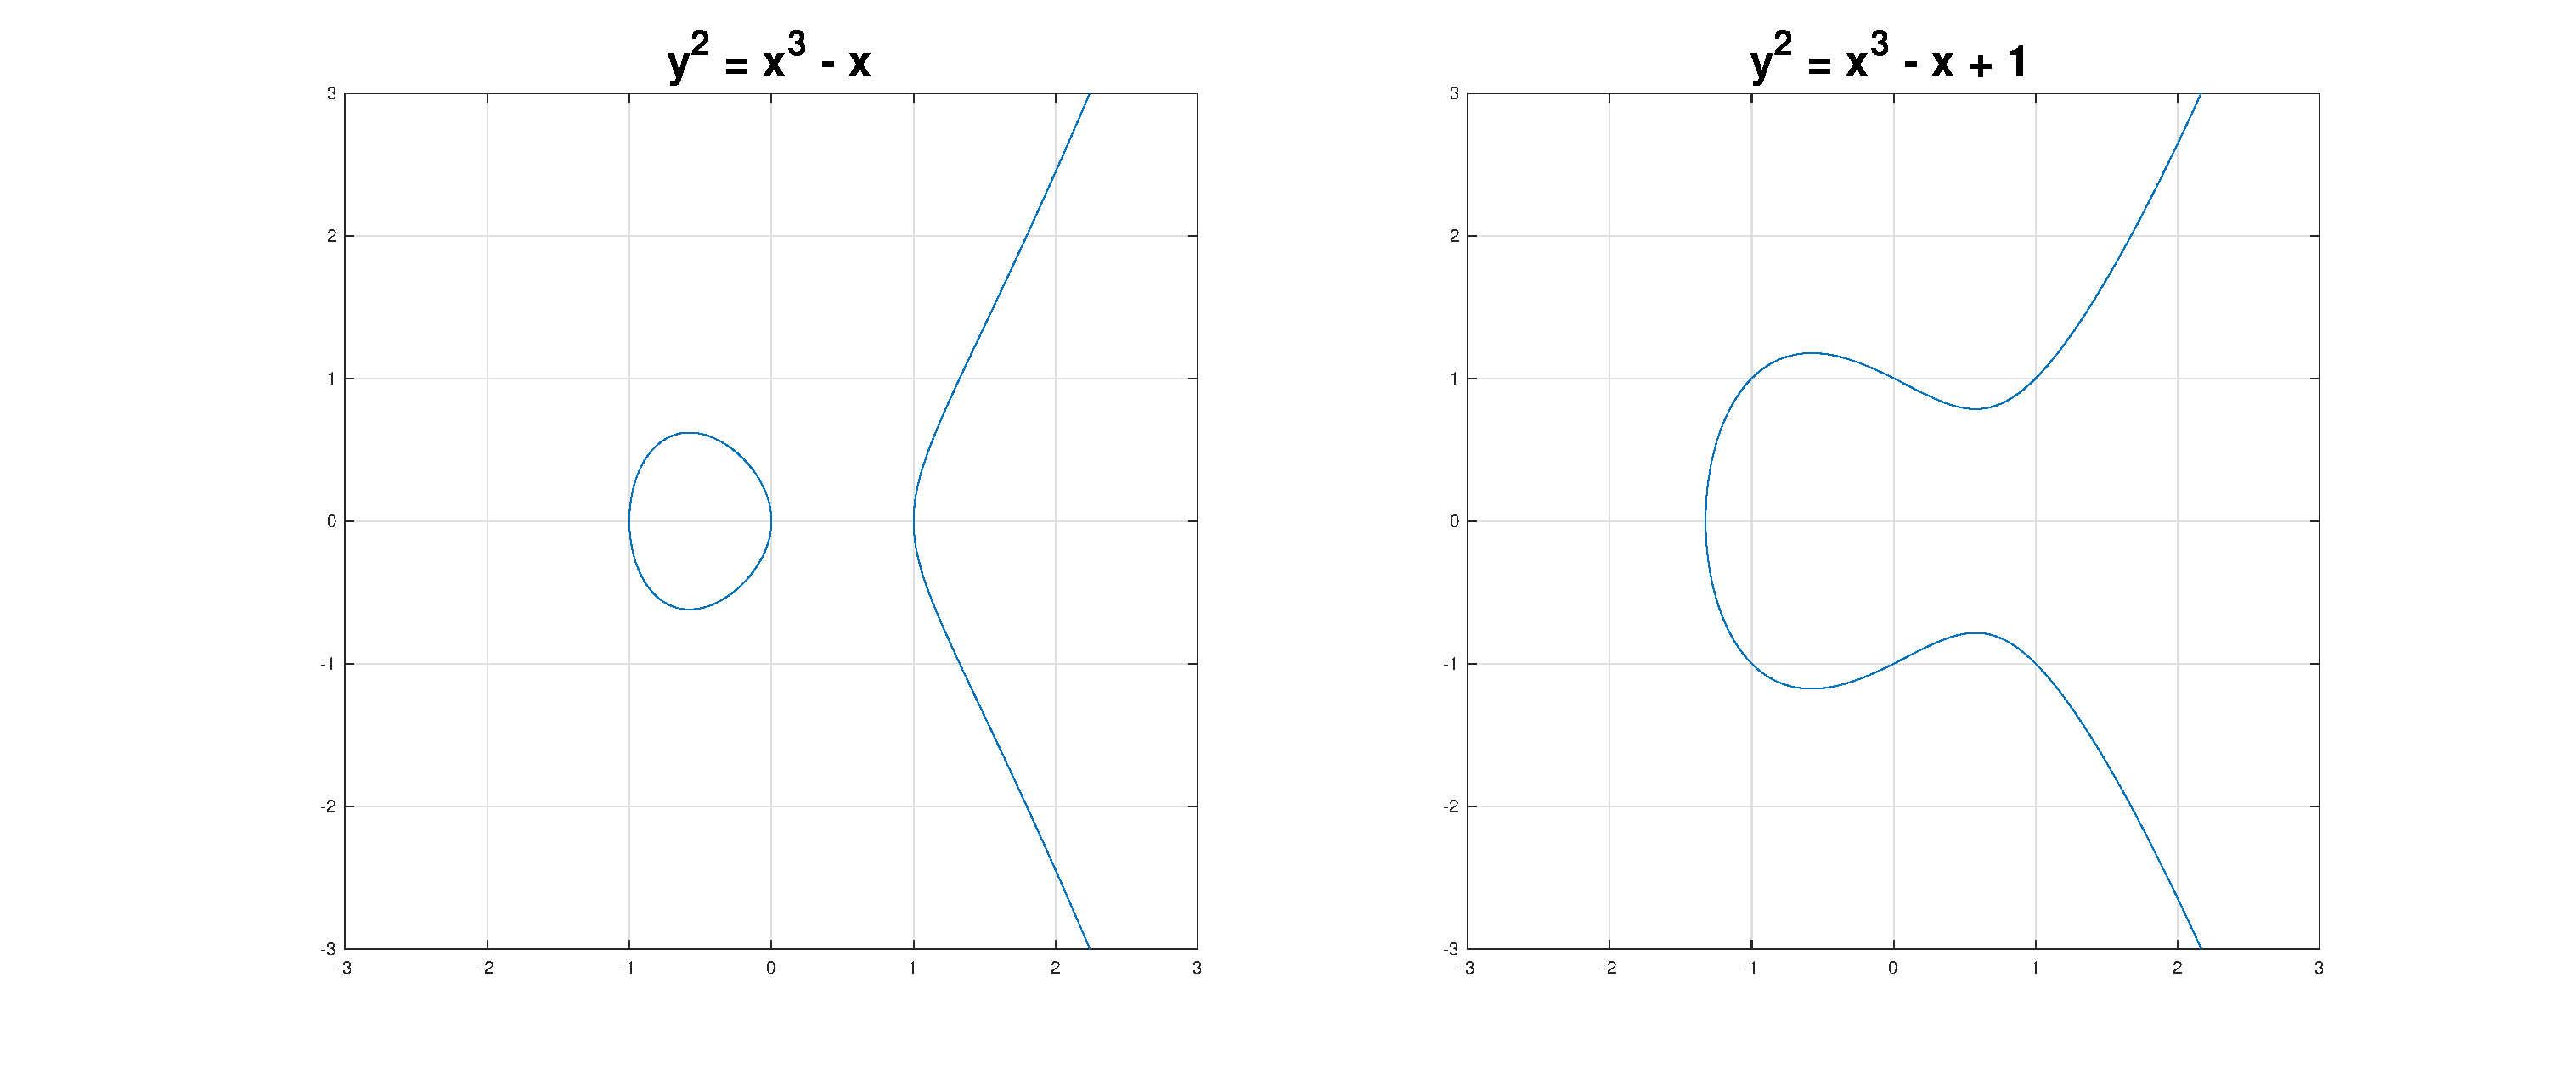
\includegraphics[width=15cm, height=7cm]{Images/EC.eps}}
	\captionof{figure}{Two examples of elliptic curves over the real numbers.}
	\label{fig:figure1}
	\source{\url{https://en.wikipedia.org/wiki/Elliptic_curve\#Elliptic_curves_over_the_real_numbers}.}
\end{figure}
\noindent
As we can see, the elliptic curves are symmetric with respect to the $x$-axis, so that for every feasible $x$ there are two $y$ values satisfying the Weierstrass equation.
\\
Typically the Weierstrass equation is coupled with the constraint that the discriminant of the cubic $x^3 + ax + b$ is different from zero. This is equivalent to ask that:
$$4a^3 + 27b^2 \neq 0,$$ 
in order to avoid multiple roots. Geometrically, this requirement means that there are no cusps, self intersections or isolated points\footnote{This requirement has also other implications: it can be shown that, without it, the elliptic curve $E_{ns}(K)$ defined over the non-singular points has an isomorphism with simpler algebraic structures, such as $K$ itself or $K^{\times}$. This problem typically arises when dealing with elliptic curves modulo composites.}. 
We can also link the sign of the discriminant to the number of components of the curve: the real graph of a curve has two components if its discriminant is positive, and one component if it is negative, as exemplified in Figure \ref{fig:figure1} (the discriminant is $\Delta = -16(4a^3 + 27b^2)$).

\bigskip
\noindent
We get back for a moment to the generalized Weierstrass equation, and show how to go from there to the more appealing Weierstrass form:
$$y^2 + a_1xy + a_2y = x^3 + a_3x^2 + a_4x + a_5,$$ 
with $a_1,...,a_5$ constants in $K$. We have said that this is the most generic form for an elliptic curve, but what does it exactly mean? It means that it is always possible to reduce to the Weierstrass equation, unless the characteristic of the field over which the curve is defined is two or three. In these two cases, we need to resort to the general formula.
\\
However, if the characteristic of the field is not two we can divide by two\footnote{Remember that in a field of characteristic two the number two acts as zero, the additive element that has not a multiplicative inverse.} and complete the square: $$\left(y + \frac{a_1x}{2} + \frac{a_2}{2}\right)^2 = x^3 + \left(a_3 + \frac{a_1^2}{4}\right)x^2 + \left(a_4 + \frac{a_1a_2}{2}\right)x + \left(\frac{a_2^2}{4} + a_5\right),$$ which can be written as $$y_1^2 = x^3 + a_1{'}x^2 + a_2{'}x + a_3{'},$$ with $y_1 = y + \frac{a_1x}{2} + \frac{a_2}{2}$ and new constants $a_1{'}, a_2{'}, a_3{'} \in K$. Moreover, if the characteristic is neither three, then we can consider $x_1 = x + \frac{a_1{'}}{3}$:
$$y_1^2 = x^3 + a_1{'}x^2 + a_2{'}x + a_3{'} = \left(x_1 - \frac{a_1{'}}{3}\right)^3 + a_1{'}\left(x_1 - \frac{a_1{'}}{3}\right)^2 + a_2{'}\left(x_1 - \frac{a_1{'}}{3}\right) + a_3{'} = $$ $$= \left(x_1 - \frac{a_1{'}}{3}\right)\left(x_1^2 + \frac{a_1{'}^2}{9} -\frac{2}{3}a_1{'}x_1 + a_1{'}x_1 - \frac{a_1{'}^2}{3} + a_2{'}\right) + a_3{'} = $$ $$=\left(x_1 - \frac{a_1{'}}{3}\right) \left(x_1^2 + \frac{1}{3}a_1{'}x_1 - 	\frac{2}{9}a_1{'}^2 + a_2{'}\right) + a_3{'} = $$ $$= x_1^3 + \cancel{\frac{1}{3}a_1{'}x_1^2} - \frac{2}{9}a_1{'}^2x_1 + a_2{'}x_1 - \cancel{\frac{1}{3}a_1{'}x_1^2} - \frac{1}{9}a_1{'}^2x_1 + \frac{2}{27}a_1{'}^3 - \frac{1}{3}a_1{'}a_2{'} + a_3{'} = $$ $$=x_1^3 + \left(a_2{'} - \frac{1}{3}a_1{'}^2\right)x_1 + \left(\frac{2}{27}a_1{'}^3 - \frac{1}{3}a_1{'}a_2{'} + a_3{'}\right).$$ 
Through a proper renaming of the constants we get finally to the well known Weierstrass form: $y_1^2 = x_1^3 + ax_1 + b$ for some constants $a$ and $b$ in $K$. 
\\
Finally, for the sake of completion, we present the case of the equation $cy^2 = dx^3 + ax + b$ and how to transform it in Weierstrass form. We can multiply both sides by $c^3d^2$ and write $(c^2dy)^2 = (cdx)^3 + (ac^2d)(cdx) + bc^3d^2$. The change of variables $y_1 = c^2dy$ and $x_1 = cdx$ yields to the desired formulation of the equation.

\bigskip

\bigskip

\subsection{The group law}
\label{grouplaw}
This section is devoted to the definition of the addition operation between elements in $E(K)$: this operation turns out to be fundamental since it induces the structure of abelian group on the elliptic curve's point. Moreover, we will see why, in the definition of the curve, we had to consider the point at infinity.
\\
In particular we will consider $K$ to be the set of real numbers, in order to give an easy graphical representation of the operation. This can be done without loss of generality, since the formulas that we will derive can be shown to be valid for every $K$ with $\text{char}(K) \neq 2, 3$. 

\bigskip
\noindent
Loosely speaking we can say that:
\begin{itemize}
	\item The points of the elliptic curve are the group's elements;
	\item The identity element is the point at infinity, denoted by $\infty$;
	\item The inverse of a point $Q$ is the one symmetric about the $x$-axis: $Q = (x, y) \Longrightarrow -Q = (x, -y)$;
	\item Addition is given by the following rule: given three aligned points on the curve $Q_1$, $Q_2$ and $Q_3$ their sum is $Q_1 + Q_2 + Q_3 = \infty$.  
\end{itemize}

\begin{center}
	\noindent
	\makebox[\textwidth]{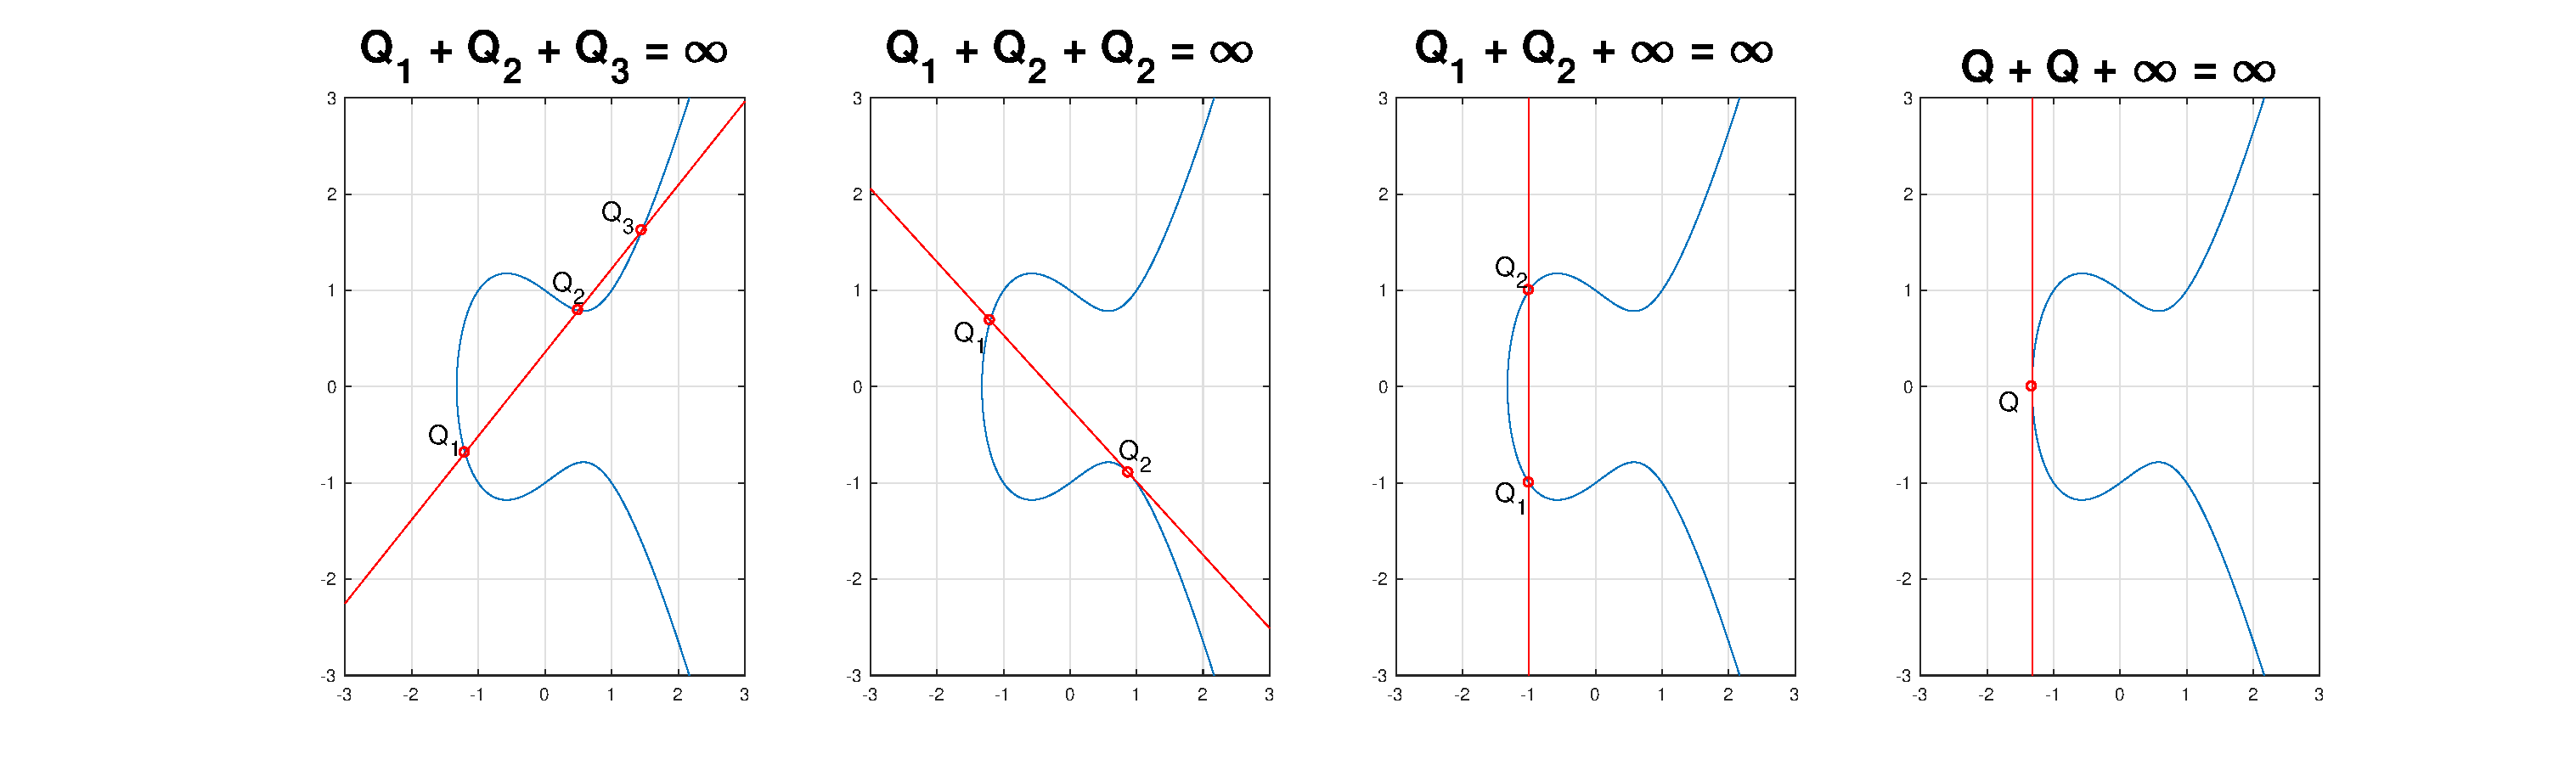
\includegraphics[width=20cm, height=5cm]{Images/chord.eps}}
	\captionof{figure}{Geometric interpretation of the addition of EC points.}
	\label{fig:figure2}
	\source{\url{https://en.wikipedia.org/wiki/Elliptic_curve\#The_group_law}.}
\end{center}
\noindent
In order to define properly the addition of EC points we need to consider five different cases. We start taking an elliptic curve $E$ defined by the usual equation in Weierstrass form $y^2 = x^3 + ax + b, \ a,b \in \mathbb{R}$ and two points $Q_1 = (x_1, y_1), \ Q_2 = (x_2, y_2) \in E(\mathbb{R})$. Unless otherwise specified, we assume also that $Q_1, Q_2 \neq \infty$.
\begin{enumerate}
	\item $x_1 \neq x_2$: consider the line passing through $Q_1$ and $Q_2$. In most of the cases (i.e. when neither the points are tangent points) this line will intersect the curve in a third point, that we denote as $-Q_3$. Then take the reflection with respect to the $x$-axis (i.e. change the sign of the $y$ coordinate): denote this final point as $Q_3$.
	\\
	The algorithm specified allows us to give meaning to the formula: 
	$$Q_1 + Q_2 = Q_3.$$
	The one outlined above is the geometrical intuition, but we can obtain algebraic formulas for the operation. The line passing through $Q_1$ and $Q_2$ has equation $y = m(x - x_1) + y_1$, where $m = \frac{y_2 - y_1}{x_2 - x_1}$ is its slope. Notice that if $x_1 = x_2$ the line is vertical, but we will treat this case later on. We can find the intersections between the line and the curve through a substitution: $(m(x - x_1) + y_1)^2 = x^3 + ax + b$. We have $m^2(x^2 - 2x_1x + x_1^2) + 2my_1(x - x_1) + y_1^2 = x^3 + ax + b$; this formula can be rearranged in the form: $$x^3 - m^2x^2 + (a + 2m^2x_1 - 2my_1)x + (b + 2my_1x_1 - m^2x_1^2 -y_1^2) = 0.$$
	\\
	In general solving a cubic equation is non trivial, but we have already two roots, namely $x_1$ and $x_2$ since $Q_1$ and $Q_2$ are points on both the line and the curve. To find the third root we notice that, given a cubic polynomial $x^3 + ax^2 + bx + c$ with roots $r, s$ and $t$, we can write: $$x^3 + ax^2 + bx + c = (x - r)(x - s)(x - t) =$$ 
	$$= x^3 - (r + s + t)x^2 + (rs + rt + st)x - rst.$$
	Therefore $r + s + t = - a$, so that, if we know two roots $r$ and $s$, we can find the third as $t = - a - r - s$.
	\\
	In our case we have $x_1 + x_2 + x_3 = m^2 \ \Longrightarrow \ x_3 = m^2 - x_1 - x_2$. Remembering to change the $y$ coordinate of the intersection point due to the reflection, we get $Q_3$ as: $x_3 = m^2 - x_1 - x_2$ and $y_3 = m(x_1 - x_3) - y_1$.
	\begin{figure}
		\noindent
		\makebox[\textwidth]{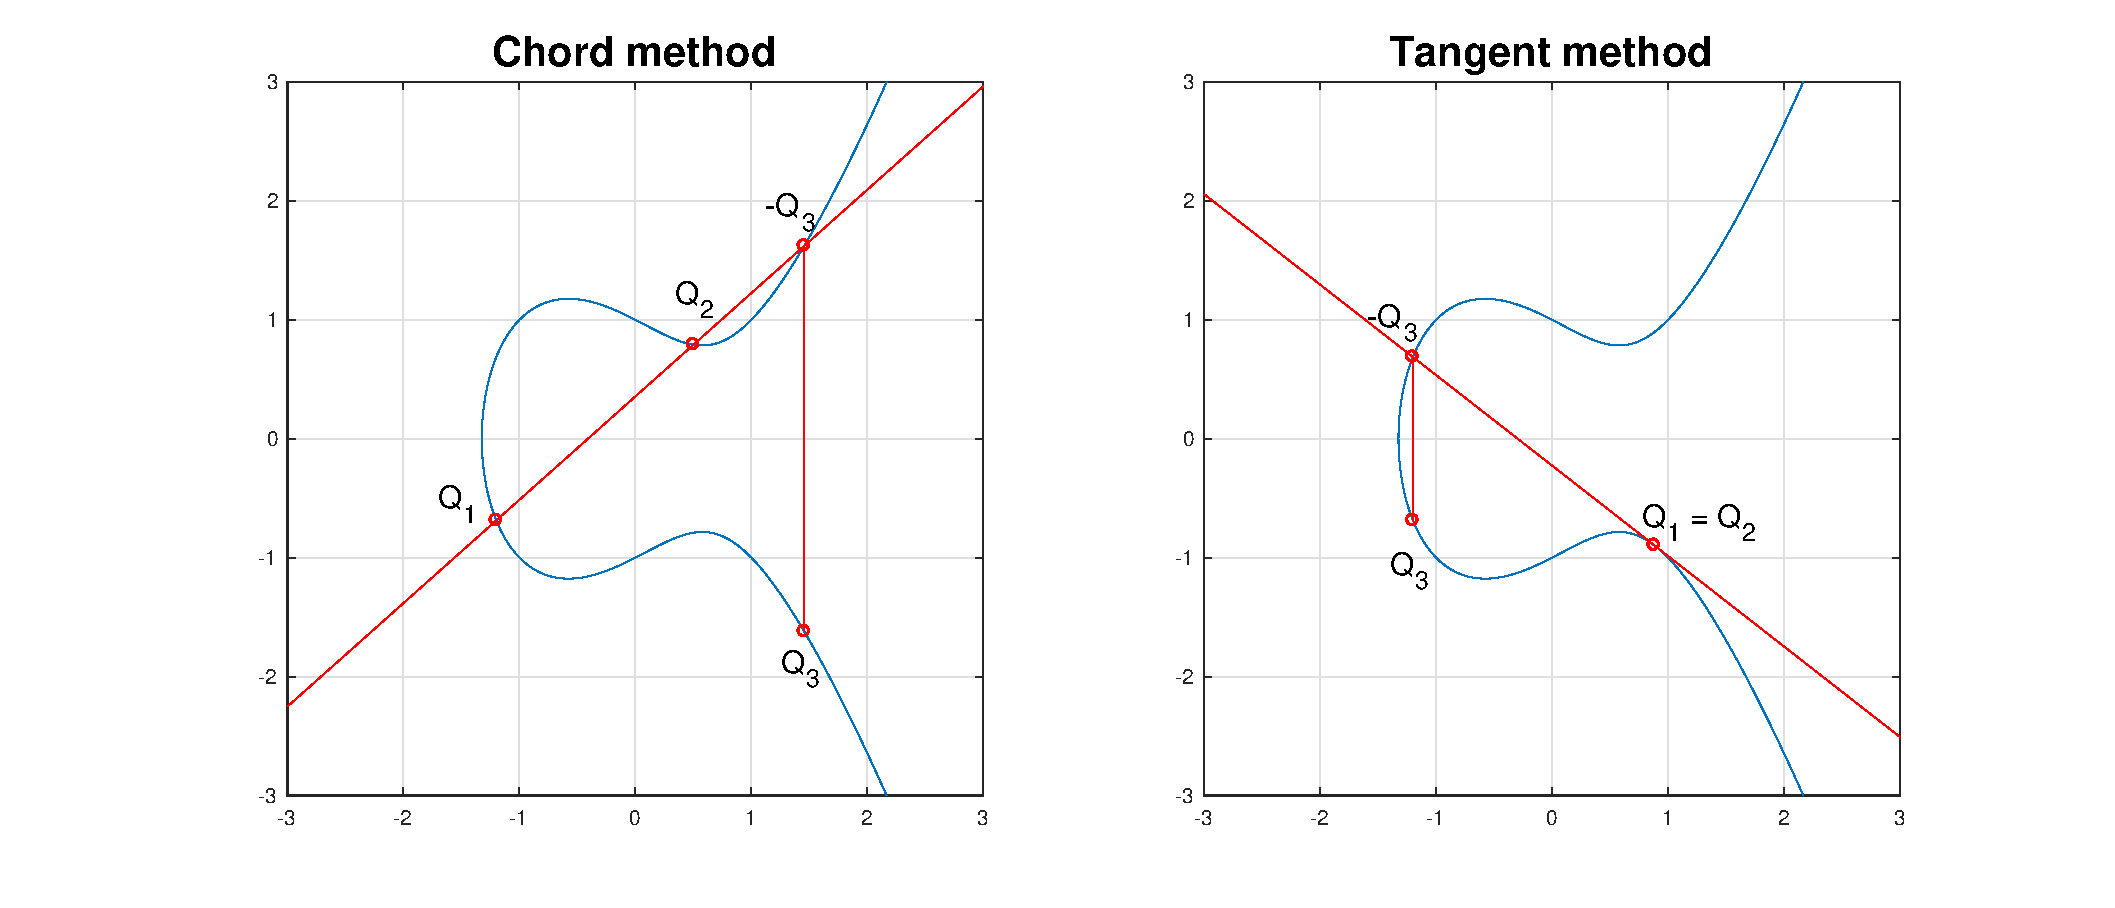
\includegraphics[width=15cm, height=7cm]{Images/sum.eps}}
		\captionof{figure}{Graphical representation of the point addition.}
		\label{fig:figure3}
	\end{figure}
	
	\item $x_1 = x_2 \wedge y_1 \neq y_2$: the line through $Q_1$ and $Q_2$ is vertical, therefore it intersects $E$ at $\infty$. Reflecting the point at infinity across the $x$-axis yields to the same point. Therefore, in this case $Q_1 + Q_2 = \infty$. 
	\\
	This is in agreement with what we stated before: if  $x_1 = x_2 \wedge y_1 \neq y_2$ it means that $Q_2 = -Q_1$, and since the point at infinity acts as the identity element we have exactly that $Q_1 + Q_2 = \infty$.
	
	\item $Q_1 = Q_2 = (x_1, y_1) \wedge y_1 \neq 0$: when two points on a curve are very close one another, the line through them approximates a tangent line. Therefore, when the two points coincide, we take the line through them to be the tangent line. Implicit differentiation allows us to find its slope $m$:
	$$y^2 = x^3 + ax + b \ \Longrightarrow \ \frac{d(y(x)^2)}{dx} = \frac{d}{dx}(x^3 + ax + b) \ \Longrightarrow$$
	$$ \Longrightarrow \ \frac{d(y^2)}{dy}\frac{dy}{dx}=2y\frac{dy}{dx}= 3x^2 + a \ \Longrightarrow $$ 
	$$\Longrightarrow \ m = \left(\frac{dy}{dx}\right)_{x_1} = \frac{3x_1^2 + a}{2y_1}.$$
	Again, the equation of the line is $y = m(x - x_1) + y_1$. At this point we can proceed as before: the line intersects the curve in a second point. Substituting the equation of the straight line would result in a cubic equation. But we already know two roots, so that we get: $x_3 = m^2 - 2x_1$ and $y_3 = m(x_1 - x_3) - y_1$.
	\\
	\item $Q_1 = Q_2 = (x_1, y_1) \wedge y_1 = 0$: as we can see from the previous point in this case the tangent line is vertical and we set $Q_1 + Q_2 = \infty$.
	\item The last case we have to deal with is when one of the two points is $\infty$. Suppose, without loss of generality, that $Q_2 = \infty$; the line through $Q_1$ and $\infty$ is a vertical line that intersects $E$ in the point $-Q_1$, which is the reflection of $Q_1$ across the $x$-axis. When we reflect $-Q_1$ to get $Q_3 = Q_1 + Q_2$, we get back to $Q_1$. Therefore:
	 $$Q_1 + \infty = Q_1$$
	for all points $Q_1$ on $E$. Of course, we extend this to include $\infty + \infty = \infty$.
\end{enumerate}
Thanks to these algebraic formulas we can notice that when $Q_1$ and $Q_2$ have coordinates in a field $K$ that contains $a$ and $b$, then $Q_1 + Q_2$ also has coordinates in $K$. This means that $E(K)$ is closed under the defined addition operation.

\bigskip
\noindent
Now we state a theorem showing formally that the couple $(E, +)$ is indeed an abelian group. The theorem with the proof can be found in \cite{RefWork:1}.
\begin{thm} The operation $+$ as defined above on an elliptic curve $E$ satisfies the following properties:
	\begin{enumerate}
		\item Commutativity: $Q_1 + Q_2 = Q_2 + Q_1, \ \forall Q_1, Q_2 \in E$;
		\item Identity: $Q + \infty = Q, \ \forall Q \in E$;
		\item Invertibility: $\forall Q \in E, \ \exists Q' \in E \ | \ Q + Q' = \infty$. This point will be denoted by $-Q$;
		\item Associativity: $(Q_1 + Q_2) + Q_3 = Q_1 + (Q_2 + Q_3), \ \forall Q_1, \ Q_2, Q_3 \in E$.
	\end{enumerate}
\end{thm}

\bigskip
\noindent
Although we won't prove the theorem, it can be useful to give a sketch of its proof. The commutativity is obvious, either from the formulas or from the fact that the line passing through $Q_1$ and $Q_2$ is the same as the line passing through $Q_2$ and $Q_1$. The identity property of the point at infinity holds by definition, as the existence of the inverse element.
\\
The tricky part of the proof is related with associativity: either it can be proved working out the annoying computations or through a much more elegant and complex method based on projective coordinates, for which we again refer to the bibliography.

\bigskip
\noindent
Now that we have clear in mind what does addition between EC points mean, we can define subtraction and scalar multiplication:
\begin{itemize}
	\item Subtraction: given $Q, R \in E$, we set $Q - R = Q + (-R)$. We can do this since everything is perfectly defined in the right hand side of the equation;
	\item Scalar multiplication: $\forall k \in \mathbb{N}$\textbackslash$\{0\}, \ kQ = Q + Q + ... + Q$, where the addition is repeated $k - 1$ times.
\end{itemize}
Notice that to compute the scalar multiplication for a large $k$ it is inefficient to add $Q$ to itself repeatedly. There are several faster approaches, the simplest called the {\bf Double and Add Algorithm}. 
We stress this fact since, as we will see later on, scalar multiplication and its computational asymmetry are the key ingredients for elliptic curve cryptography: the fact is that it is easily computable\footnote{The double and add algorithm requires polynomial time in the number of bits $n$ representing the numbers involved, compared to the exponential time required by the naive approach; that is, assuming that the point doubling and the point addition require a constant time, we need $O(n^{\alpha}), \ \alpha > 1$ elementary operations, compared to $O(2^n)$. In particular on average it requires $n$ doublings and $0.5 * n$  additions, since the binary expansion of a random integer has an equal number of 1's and 0's.}
but its inversion, the so called discrete logarithm (DL), although not provable to be hard, is believed to be so: this means that in general we have no efficient algorithm to compute it.
\\
\\
{\bf Double and Add Algorithm}: To compute $kQ$, start with the binary representation of $k$: $k = k_0 + 2k_1 + 2^2k_2 + ... + 2^nk_n$, where $k_0,...,k_n \in \{0, 1\}$. 

\begin{algorithm}
	\caption{Double and Add algorithm}
	\label{alg:double_add}
	\begin{algorithmic}[1]
		\Procedure{double\_and\_add}{$k, \ Q$}
		\State $R \gets \infty$
		\For {$i\gets 1,n$}
		\If{$k_i = 1$}
		\State $R \gets Q + R$
		\EndIf
		\State $Q \gets Q + Q$
		\EndFor
		\State \textbf{return} $R$
		\EndProcedure
	\end{algorithmic}
\end{algorithm}
\noindent
The algorithm can be further sped up through the pre-computation of a vector of multiples of $Q$: this approach is not always feasible, since the point $Q$ is not always fixed\footnote{The point $Q$ is fixed, for example, when computing the public key from a private key. For a thorough exposition of these concepts we refer to Chapter \ref{chpr:ecc}.}.
\chapter{Elliptic curve cryptography}
\label{chpr:ecc}
In this chapter we will analyse the cryptographic primitives and assumptions that will allow in the next chapter to introduce the digital signature schemes that are the core of the present work. The first argument will be the specialization of elliptic curves to finite fields, the mathematical structure underpinning the whole elliptic curve cryptography.

\bigskip

\section{Elliptic curves over finite fields}
\label{ecoverff}
Up to now we considered the field over which the curve is defined to be the set of real numbers: this is not at all the unique possibility. The typical choice in cryptography is $K = \mathbb{F}_p$, where $\mathbb{F}_p$ is the finite field with $p$ elements. 
\\
Since there are only finitely many pairs $(x, y)$ with $x, y \in \mathbb{F}_p$, the group $E(\mathbb{F}_p)$ is finite.
In practice we consider: 
$$\{(x, y) \in \mathbb{F}_p^2 \ | \ y^2 \equiv x^3 + ax + b \ (\text{mod} \ p), \ 4a^3 + 27b^2 \not\equiv 0 \ (\text{mod} \ p)\} \cup \{\infty\}.$$
It can be shown that the formulas for point addition are the same derived in Section \ref{grouplaw}, but where the calculations are done modulo $p$\footnote{Notice that reduction modulo $p$ can be executed much faster if the prime $p$ is a Mersenne or a pseudo-Mersenne prime, i.e. if $p = 2^d - 1$ for some $d$ in the first case or if $p \simeq 2^d$ in the second one.}.
\\
\begin{center}
	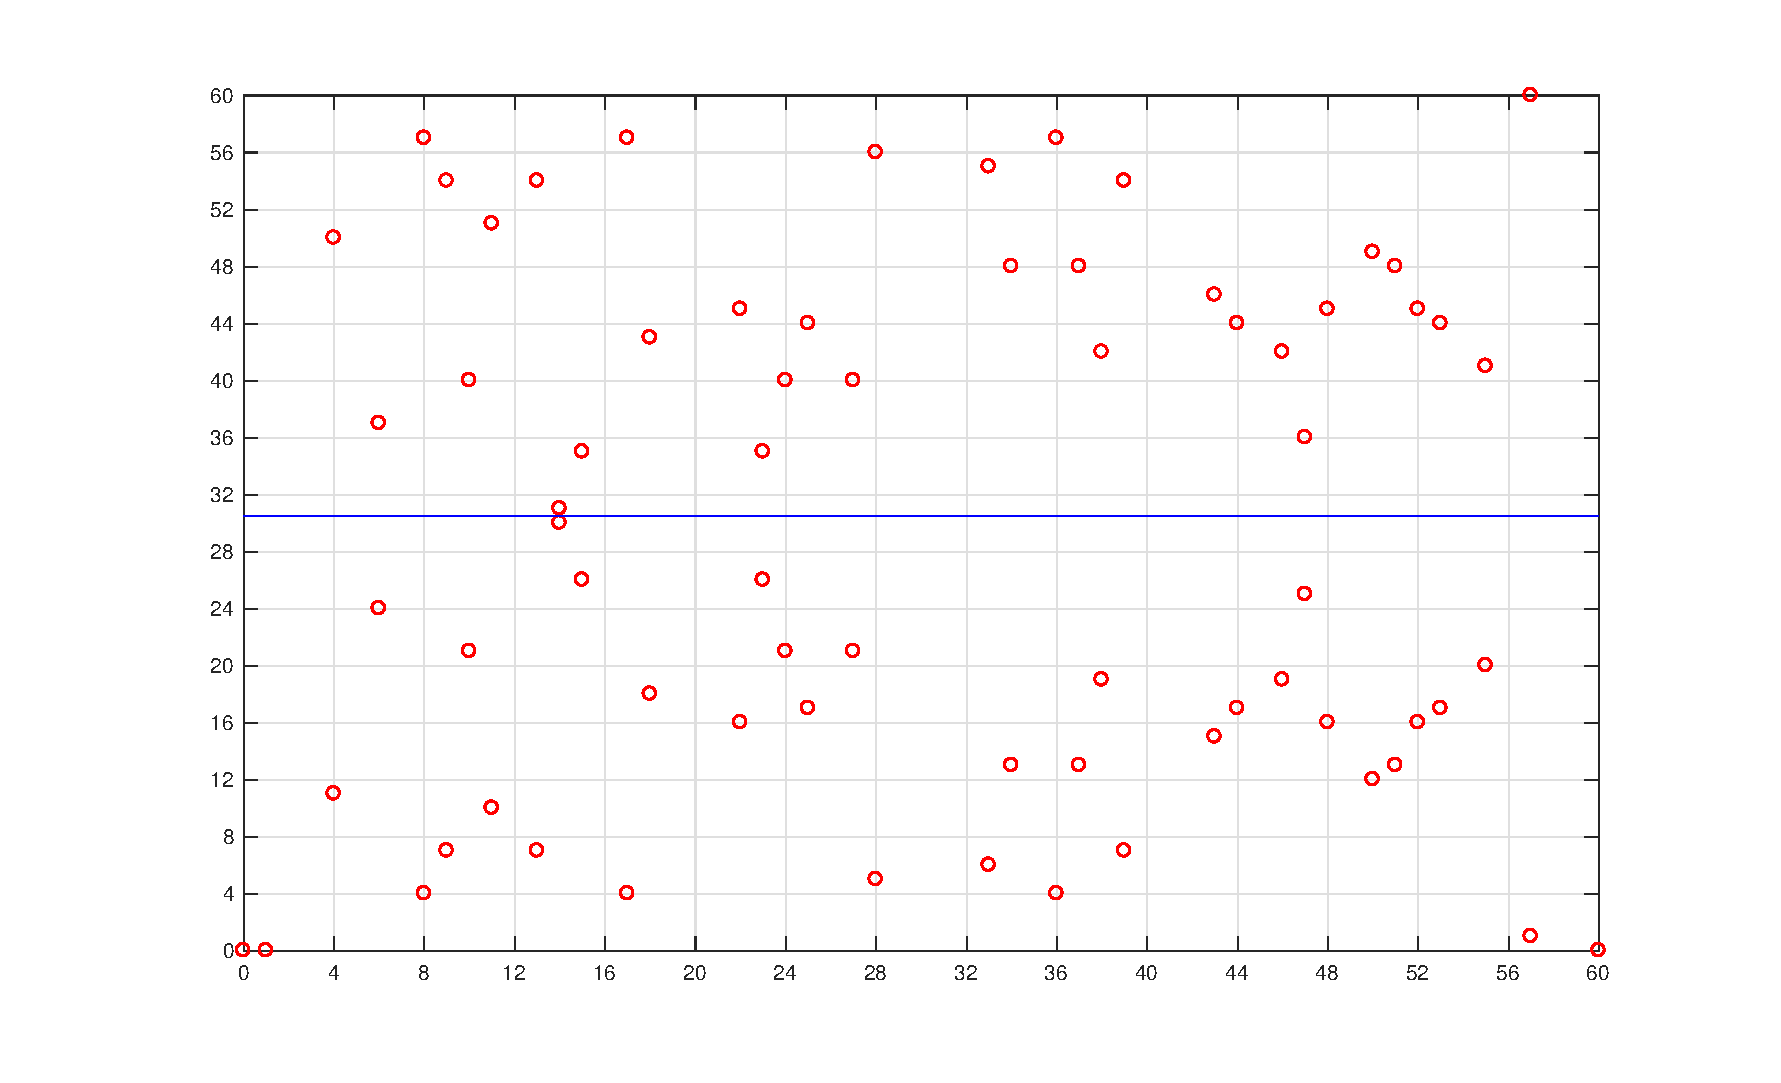
\includegraphics[width=0.9\linewidth]{Images/ec_over_ff.eps}
	\captionof{figure}{The curve $y^2 = x^3 - x$ over $\mathbb{F}_{61}$.}
	\label{fig:figure4}
	\source{\url{https://en.wikipedia.org/wiki/Elliptic_curve\#Elliptic_curves_over_finite_fields}.}
\end{center}
In Figure \ref{fig:figure4} the typical shape of an elliptic curve over a finite field is represented: we can see that we are not anymore dealing with a smooth curve, but with a finite set of points scattered along the plane. We can notice a certain degree of symmetry with respect to the line $y = \frac{p}{2}$, with the exception of the points with $y$ coordinate equal to zero, that correspond to the roots of the cubic $x^3 + ax + b$ in $\mathbb{F}_p$.
\\
It is still possible to define a geometric method for point addition: the general idea is that we draw the line passing through the points considered. Since we are working in modular arithmetic, this line "repeats" itself along the plane. Once the line intersects a third point, we take the opposite one to be the result of the addition. The approach is presented in Figure \ref{fig:figure5}, however the method can be somewhat counterintuitive, especially when dealing with point doubling, so we stick with the algebraic notation.

\bigskip
\noindent
The number of points on an EC over $\mathbb{F}_q$ plays a central role in the cryptographic applications, so we state here a useful theorem that allows to give an estimate:
\begin{thm} [{\bf Hasse's theorem}] Let $\mathbb{F}_q$ be a finite field and let $E$ be an elliptic curve defined over $\mathbb{F}_q$. Then the order of $E(\mathbb{F}_q)$ (i.e. the number of points) satisfies: $$|q + 1 - \#E(\mathbb{F}_q)| \leq 2\sqrt{q}.$$
\end{thm}
\begin{center}
	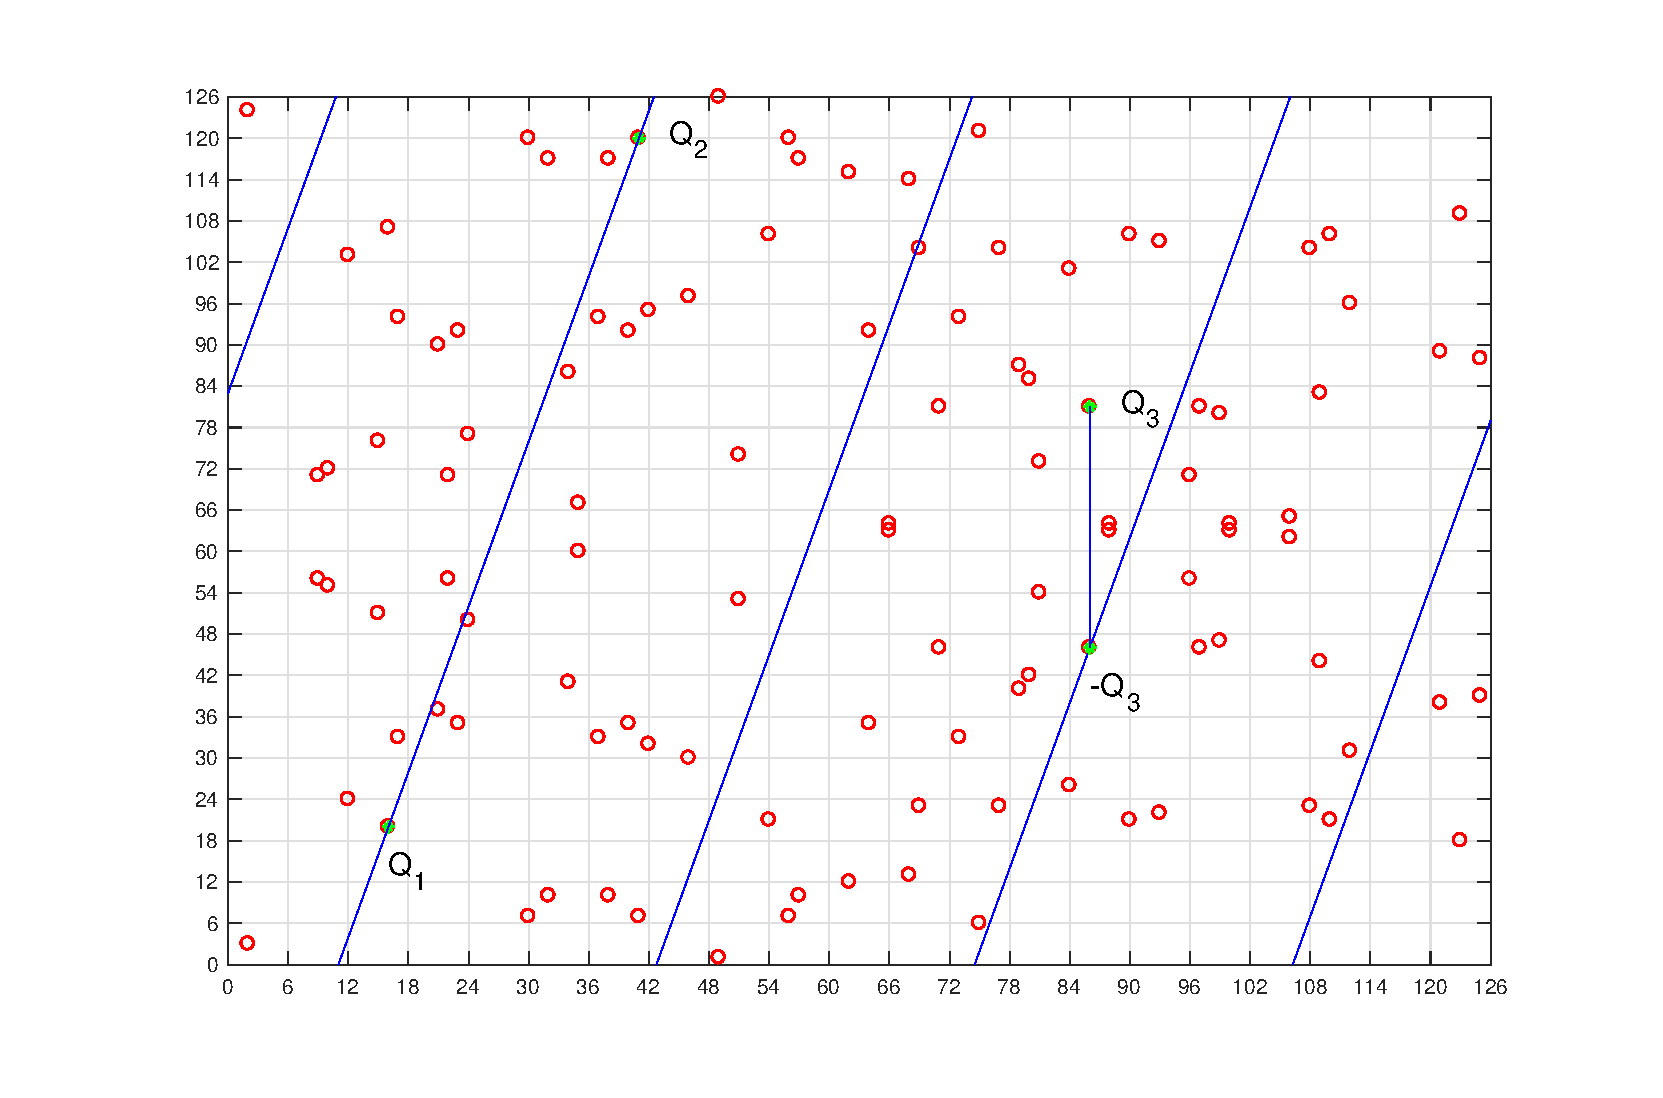
\includegraphics[width=0.9\linewidth]{Images/sum_ec_over_ff.eps}
	\captionof{figure}{Geometric representation for the addition of points on the elliptic curve $y^2 = x^3 - x + 3$ over $\mathbb{F}_{127}$.}
	\label{fig:figure5}
	\source{\cite{RefWork:4}.}
\end{center}
\noindent
Loosely speaking, Hasse's theorem tells us that the number of points over $E(\mathbb{F}_q)$ increases linearly with the order of the field.
\\
Another observation we want to do is that if $\#E(\mathbb{F}_p)$ is a prime number, then $E(\mathbb{F}_p)$ is a cyclic group: this is a direct consequence of Lagrange's theorem. Since the order of each subgroup is a divisor of the order of the group, we have that, if the order of the group is a prime number, there is no subgroup (with the exception of the trivial one, comprising only the point at infinity). This means that it has to exist a generator of the whole group. Suppose this is not the case, i.e. $\nexists G \in E(\mathbb{F}_p) \ | \ \forall Q \in E(\mathbb{F}_p) \ \exists q \in [1, ..., \#E(\mathbb{F}_p)] \ \text{s.t.} \ Q = qG$: thus, $\forall G \in E(\mathbb{F}_p)$, there exists at least a $Q$ for which the relation $Q = qG$ does not hold. Fix $G$ and start adding it repeatedly to itself. Of course we would reach different points in $E(\mathbb{F}_p)$ due to the closure of the addition. However we won't be able to reach $Q$, by definition. But eventually we would reach the point at infinity (when $q$ gets equal to the order of $G$): then we would start again, meaning that we would have found a cyclic subgroup. But this is in contrast with Lagrange's theorem, so that we can conclude that the whole set of elliptic curve's points form a cyclic group if $\#E(\mathbb{F}_q)$ is a prime number.

\bigskip

\subsection{Elliptic curve domain parameters}
\label{ecparam}
In order to rely on ECC, the parties involved in a scheme need to agree on a set of parameters called elliptic curve domain parameters. A typical choice is to rely on standardized curves (e.g. those defined in \cite{RefWork:3}); however, it is still possible to choose other parameters, but this has to be done carefully, as we will explain in this section. We start defining EC parameters, following closely \cite{RefWork:2}.
\\
\\
Elliptic curve parameters are defined as a sextuple $T = (p, a, b, G, n, h)$, where:
\begin{itemize}
	\item The integer $p$ specifies the prime finite field $\mathbb{F}_p$;
	\item The two elements $a, b \in \mathbb{F}_p$ specifies the elliptic curve $E(\mathbb{F}_p)$ through the Weierstrass equation;
	\item $G$ is a point on $E(\mathbb{F}_p)$;
	\item $n$ is the order of $G$, i.e. the number of elements of the cyclic subgroup generated by $G$ (that can coincide with the whole $E(\mathbb{F}_p)$);
	\item $h = \frac{\#E(\mathbb{F}_p)}{n}$ is an integer\footnote{We can deduce that $h$ is an integer directly from Lagrange's theorem.} called the cofactor. 
\end{itemize}
There are different ways in which we can choose these parameters. For example, they can be generated at random or not. Random generation is a conservative choice, since it offers a guarantee against future special purpose attacks. In this case it could be better to use verifiable random parameters, meaning that $(a, b)$ and/or $G$ are obtained as output from a secure hash function\footnote{An hash function in general is a function that takes as input strings of arbitrary length and outputs in a fixed length sequence of bytes. For a discussion on the security properties of an hash function we refer to the appendix of \cite{RefWork:2}.}, applied to some seed $S$. When choosing verifiable random parameters, the sextuple $T$ should be coupled with the seed value $S$ to allow parameters' validation. However, non random curves are typically built in particular ways to ensure efficient computations. Standardized curves, that comprises both types of EC, have the advantage of underpinning interoperability, plus an high degree of reliability, having been heavily tested.
\\
Now that we have explained what they are and how they can be chosen, we will show some constraints and the validation process for the sextuple $T$.

\bigskip
\bigskip
\bigskip
\bigskip
\bigskip
\noindent
{\bf Parameters' selection}: 
\begin{enumerate}
	\item Select the approximate security level in bits, $t$\footnote{The security level should be chosen such that solving the ECDLP requires $2^t$ curve's operations. The SEC standard that we are following restricts to $t \in \{80, 112, 128, 192, 256\}$.};
	\item Choose a prime $p$ such that $\lceil log_2p\rceil = 2t$ if $80 < t < 256$, such that $\lceil log_2p\rceil = 521$ if $t = 256$ and such that $\lceil log_2p\rceil = 192$ if $t = 80$;
	\item Select $a$ and $b$ in $\mathbb{F}_p$ such that:
	\begin{itemize}
		\item $4a^3 + 27b^2 \neq 0 \ (\text{mod} \ p)$;
		\item $\#E(\mathbb{F}_p) \neq p$;
	\end{itemize} 
	\item Select $G \in E(\mathbb{F}_p)$ such that:
	\begin{itemize}
		\item $p^B \neq 1 \ (\text{mod} \ n), \ \forall 1 \leq B < 100$;
		\item $h \leq 2^{\frac{t}{8}}$;
		\item $n - 1$ and $n + 1$ should each have a large prime factor $r$, which is large in the sense that $log_nr > \frac{19}{20}$.
	\end{itemize}
\end{enumerate}
These requirements may look strange, but are all needed in order to avoid special attacks. In particular, the two requirements at point 3 are needed in order for the curve to be non singular and to avoid Smart's attack\footnote{The points on the curve are mapped to the elements of the additive group of $\mathbb{F}_p$, so that the discrete logarithm problem is solvable in polynomial time through the {\bf Extended Euclidean Algorithm}.}, respectively.
\\
The three requirements at point 4 instead are needed to ensure that the curve is robust against MOV and Cheon's attack\footnote{These attacks are complex and their explanation is out of the scope of the present work; we refer the interested reader to the appendix of \cite{RefWork:2} for an overview and for further bibliography.}, and to ensure that the order of $G$ is sufficiently high.
\\
Notice however that the choice of the parameters does not secure against all possible attacks. Indeed other kind of attacks may be possible, such as side channel attacks: timing and power analysis are an example. They exploit the differences in the point addition and doubling operations, that lead to different timings or power consumptions. Possible solutions are a change of coordinates or the use of Edwards curves, a special family of elliptic curves for which addition and doubling can be done with the same operation.

\bigskip
\noindent
{\bf Parameters' validation}: Given $T = (p, a, b, G, n, h)$ and $t$, the parameters are deemed valid if:
\begin{enumerate}
	\item $p$ is a prime such that $\lceil log_2p\rceil = 2t$ if $80 < t < 256$, or such that $\lceil log_2p\rceil = 521$ if $t = 256$, or such that $\lceil log_2p\rceil = 192$ if $t = 80$;
	\item $a, b, x_G$ and $y_G$ are integers in $[0, ..., p - 1]$;
	\item $4a^3 + 27b^2 \neq 0 \ (\text{mod} \ p)$;
	\item $y_G^2 = x_G^3 + ax_G + b \ (\text{mod} \ p)$;
	\item $n$ is a prime number;
	\item $h \leq 2^{\frac{t}{8}}$ and $h = \lfloor (\sqrt{p} + 1)^2 / n \rfloor$;
	\item $nG = \infty$;
	\item $p^B \neq 1 \ (\text{mod} \ n), \ \forall 1 \leq B < 100$ and $n \neq p$. 
\end{enumerate}
If the parameters are verifiably random, it should also be checked that $(a, b)$ and/or $G$ have been correctly derived from the seed $S$.
\\
These checks are needed to verify that: the curve has the required difficulty level, it is defined over $\mathbb{F}_p$, it is non singular, $G$ is a point of the curve, the DL is difficult, $h$ is effectively the cofactor of $G$, $G$ has order $n$ and neither MOV nor Smart's attacks are possible.

\bigskip

\subsection{Elliptic curve key pairs}
\label{keypairs}
In this section we would like to briefly analyse the core of the public key cryptography based on elliptic curves: the concept of elliptic curve key pair. Shortly, public key cryptography is a cryptographic system that relies on pairs of keys, a public and a private key, with different roles. The asymmetry of the keys is the reason behind the fact that public key cryptography is sometimes called also asymmetric cryptography. We talk about asymmetry since public keys can be published, while private keys must be kept secret, as the names suggest. This accomplishes two functions: authentication, since everybody with the public key can verify that the holder of the paired private key sent a signed message, and encryption, where the public key is used for encryption, but only the owner of the private counterpart can decrypt.

\bigskip
\noindent
Given some elliptic curve domain parameters $T = (p, a, b, G, n, h)$, an elliptic curve key pair $\{\textcolor{red}{q}, \textcolor{green}{Q}\}$ associated with $T$ consists of an elliptic curve secret key $\textcolor{red}{q}$, which is an integer in $[1, n - 1]$, and an elliptic curve public key $\textcolor{green}{Q} = (x_Q, y_Q)$, which is the point $\textcolor{green}{Q} = \textcolor{red}{q}G$.
\\
The choice of the colours is intended to make clear what is secret and what can be made public.
\\
To detect transmission errors or to prevent the deliberate submit of an invalid key, it is desirable to validate the public key of the counterparties. This can be achieved following these steps:

either to prevent malicious insertion of an invalid public key to enable attacks like small subgroup attacks, or to detect inadvertent coding or transmission errors.

\begin{enumerate}
	\item Check that $Q \neq \infty$;
	\item Check that $x_Q$ and $y_Q$ are integers in $[0, p - 1]$ and that $y_Q^2 = x_Q^3 + ax_Q + b \ (\text{mod} \ p)$;
	\item Check that $nQ = \infty$.
\end{enumerate}
Through this algorithm we are checking that $Q$ is effectively a point on the curve different from the point at infinity and that it belongs to the cyclic subgroups generated by $G$. Indeed, if the relation $Q = qG$ holds we have that $nQ = n(qG) = q(nG) = q\infty = \infty$. If this would not be the case, the third check would fail.

\bigskip

\subsection{Jacobian coordinates}
\label{jac}
We have already written that for EC over finite fields the same formulas previously seen hold, with the calculations done modulo $p$. What we have not dealt with is that this comes with a downside: in particular we have now to deal with modular inversion, an operation that, although can be done efficiently, is up to two orders of magnitude slower than field's multiplication.
\\
In the next chapter we will deal with digital signatures and we will see that ECDSA requires modular inversion. This traduces in poor performances when it comes to a system like Bitcoin in which signatures are (potentially) verified by each participant in the network to validate transactions. Therefore, it is sometimes advantageous to avoid modular inversion, either in the formulas for point addition or in the signature scheme. The first case can be solved through a change of coordinates: the approach consists in writing all the points as points in a projective space, the key idea being to defer the divisions by multiplying them into a denominator, represented then as a new coordinate, instead of performing every division immediately. Only at the very end we perform a single division to convert from projective coordinates back to affine coordinates. 

\bigskip
\noindent
Jacobian coordinates are a modification of projective coordinates, typically used since they lead to a faster doubling procedure. In affine form, each elliptic curve point has two coordinates $(x, y)$. In projective form, each point will have three coordinates $(X : Y : Z)$, with the restriction that $Z$ is never zero for points different from the point at infinity\footnote{A projective point is denoted by $(X : Y : Z)$ since, in general, the two dimensional projective space \textbf{P}$_K^2$ over a field $K$ is given by equivalence classes of triples $(X, Y, Z)$, with $X, Y, Z \in K$ and at least one element different from zero. Here equivalence between $(X_1, Y_1, Z_1)$ and $(X_2, Y_2, Z_2)$ means that $\exists \lambda \in K \ | \ (X_1, Y_1, Z_1) = \lambda(X_2, Y_2, Z_2)$. Thus, the equivalence classes only depend on the ratios of $X$ to $Y$ to $Z$, from which the notation.}. The forward mapping is given by $(x, y) \mapsto (xz^2, yz^3, z)$, for any non zero $z$ (usually chosen to be 1 for convenience). The reverse mapping is given by $(X : Y : Z) \mapsto (X/Z^2, Y/Z^3)$, as long as $Z$ is non zero.
\\
The elliptic curve $y^2 = x^3 + ax + b$ becomes:
$$Y^2 = X^3 + aXZ^4 + bZ^6.$$
The point at infinity now has the coordinates $(1 : 1 : 0)$: indeed, substituting $Z = 0$ in the equation defining the curve we get $Y^2 = X^3$; then we simply normalize.
\\
Let $Q_i = (X_i : Y_i : Z_i), \ i = 1, 2$, be points on the elliptic curve $Y^2 = X^3 + aXZ^4 + bZ^6$. Then:
$$(X_3 : Y_3 : Z_3) = (X_1 : Y_1 : Z_1) + (X_2 : Y_2 : Z_2),$$
where $X_3,Y_3$ and $Z_3$ are computed as follows:
\begin{itemize}
	\item $Q_1 \neq \pm Q_2$: we have the affine test $x_1 = x_2$, that in jacobian coordinates correspond to the check $X_1/Z_1^2 = X_2/Z_2^2 \ \Longrightarrow \ X_1Z_2^2 = X_2Z_1^2$. 
	\\
	We start again from the slope of the line passing through $Q_1$ and $Q_2$.
	$$m = \frac{y_2 - y_1}{x_2 - x_1} = \frac{Y_2/Z_2^3 - Y_1/Z_1^3}{X_2/Z_2^2 - X_1/Z_1^2} = \frac{Y_2/Z_2^3 - Y_1/Z_1^3}{X_2/Z_2^2 - X_1/Z_1^2} \cdot \frac{Z_1^3Z_2^3}{Z_1^3Z_2^3} =$$ $$= \frac{Y_2Z_1^3 - Y_1Z_2^3}{X_2Z_1^3Z_2 - X_1Z_1Z_2^3}.$$
	Defining $T = Y_1Z_2^3$, $U = Y_2Z_1^3$, $W = U - T$, $R = X_1Z_2^2$, $S = X_2Z_1^2$ and $V = S - R$ we can write:
	$$m = \frac{U - T}{SZ_1Z_2 - RZ_1Z_2} = \frac{W}{VZ_1Z_2}.$$
	Now consider:
	$$x_3 = m^2 - x_1 - x_2 = \frac{W^2}{V^2Z_1^2Z_2^2} - \frac{X_1}{Z_1^2} - \frac{X_2}{Z_2^2} = \frac{W^2}{V^2Z_1^2Z_2^2} - \frac{X_1}{Z_1^2}\cdot\frac{V^2Z_2^2}{V^2Z_2^2} - \frac{X_2}{Z_2^2}\cdot\frac{V^2Z_1^2}{V^2Z_1^2} = $$ $$= \frac{W^2 - V^2X_1Z_2^2 - V^2X_2Z_1^2}{V^2Z_1^2Z_2^2} = \frac{W^2 - V^2R - V^2S}{V^2Z_1^2Z_2^2} = \frac{W^2 - V^2(S + R)}{V^2Z_1^2Z_2^2} = $$ $$= \frac{W^2 - V^2(S - R + 2R)}{V^2Z_1^2Z_2^2} = \frac{W^2 - V^3 - 2RV^2}{V^2Z_1^2Z_2^2},$$
	$$y_3 = m(x_1 - x_3) - y_1 = \frac{W}{VZ_1Z_2}\left(\frac{X_1}{Z_1^2} - \frac{W^2 - V^3 - 2RV^2}{V^2Z_1^2Z_2^2}\right) - \frac{Y_1}{Z_1^3} = $$ $$= \frac{W}{VZ_1Z_2}\left(\frac{V^2X_1Z_2^2 - W^2 + V^3 + 2RV^2}{V^2Z_1^2Z_2^2}\right) - \frac{Y_1}{Z_1^3} = $$ $$= \frac{W(RV^2 - [W^2 - V^3 - 2RV^2]) - V^3Y_1Z_2^3}{V^3Z_1^3Z_2^3} = $$ $$\frac{W(RV^2 - [W^2 - V^3 - 2RV^2]) - TV^3}{V^3Z_1^3Z_2^3}.$$
	Thus, we can write:
	$$X_3 = W^2 - V^3 - 2RV^2, \ Y_3 = W(RV^2 - X_3) - TV^3, \ Z_3 = VZ_1Z_2,$$
	where
	$$T = Y_1Z_2^3, \ U = Y_2Z_1^3, \ R = X_1Z_2^2, \ S = X_2Z_1^2, \ V = S - R, \ W = U - T.$$
	\item $Q_1 = Q_2$:  now we have to check if $y = 0$. This is equivalent to check whether  $Y / Z^3 = 0 \ \Longrightarrow \ Y = 0$, since $Z \neq 0$.
	$$m = \frac{3x^2 + a}{2y} = \frac{3(X/Z^2)^2 + a}{2Y/Z^3} = \frac{3X^2/Z^4 + a}{2Y/Z^3} \cdot \frac{Z^4}{Z^4} = \frac{3X^2 + aZ^4}{2YZ} = \frac{W}{2YZ},$$
	if we define $W = 3X^2 + aZ^4$.
	$$x_3 = m^2 - 2x = \frac{W^2}{4Y^2Z^2} - 2\frac{X}{Z^2} = \frac{W^2 - 8XY^2}{4Y^2Z^2} = \frac{W^2 - 2V}{4Y^2Z^2},$$ once we define $V = 4XY^2$. Moreover:
	$$y_3 = m(x - x_3) - y = \frac{W}{2YZ}\left(\frac{X}{Z^2} - \frac{W^2 - 2V}{4Y^2Z^2}\right) - \frac{Y}{Z^3} = $$ $$= \frac{W(4XY^2 - [W^2 - 2V])}{8Y^3Z^3} - \frac{Y}{Z^3} = \frac{W(4XY^2 - [W^2 - 2V]) - 8Y^4}{8Y^3Z^3} =$$ $$= \frac{W(V - [W^2 - 2V]) - 8Y^4}{8Y^3Z^3}.$$
	Finally we can write:
	$$X_3 = W^2 - 2V, \ Y_3 = W(V - X_3) - 8Y^4, \ Z_3 = 2YZ,$$
	where
	$$W = 3X^2 + aZ^4, \ V = 4XY^2.$$
	\item Once again we can consider jointly the separate cases $Q_1 = Q_2 \wedge y = 0$ and $Q_1 = -Q_2$: indeed, by definition, we have $Q_1 + Q_2 = \infty$.
\end{itemize}
Looking at the formulas we can see that no inversion is involved in the calculations. Moreover, a further speed up is possible when doubling if we set $a = -3$\footnote{This is the reason why some standardized curves make this choice for the parameter $a$.}: we have $W = 3X^2 -3Z^4 = 3(X^2 - Z^4) = 3(X + Z^2)(X - Z^2)$, which can be computed via one squaring and one multiplication rather than via three squarings.

\bigskip
\noindent
We implemented this approach in the library that can be found at \url{https://github.com/dginst/BitcoinBlockchainTechnology} to improve the efficiency of the curve's operations. The speed up checks have been performed considering the curves secp192k1, secp192r1, secp224k1, secp224r1, secp256k1, secp256r1, secp384r1 and secp521r1 as described in \cite{RefWork:3}, resulting in a scalar multiplication that is from six to seven times faster in all the cases.

\bigskip

\subsection{The Bitcoin curve: secp256k1}
\label{btccurve}
Since this work is mainly focused on applications that can be deployed in Bitcoin, we would like to present the elliptic curve over a finite field used there. This could also suggest the shape of the curves used in practice.
\\
\\
The curve is named secp256k1: the naming is not casual, and its analysis could help a better understanding of the curve's properties. It begins with {\bf sec} to denote "Standards for Efficient Cryptography", the documentation from which it is taken; then it follows a {\bf p}, denoting the use of parameters over a prime field $\mathbb{F}_p$, in contrast with the so called binary fields $\mathbb{F}_{2^m}$, denoted by the letter {\bf t}; the {\bf p} is followed by a number, 256, denoting the length in bits of the field size $p$, that suggests the difficulty of solving the DL on the curve; then in comes a {\bf k} to denote parameters associated with a Koblitz curve\footnote{The name Koblitz curve used here has the same meaning as in \cite{RefWork:3}.}, to be distinguished from an {\bf r}, that would denote the use of verifiably random parameters; at last we find the sequence number {\bf 1}, meaning that this curve is the first, actually the unique, with all these characteristics.
\\
We have already discussed the benefits of using a random curve; however, secp256k1 was constructed in a special non random way to ensure efficient computations.
\\
Here follows the sextuple $T$ defining the secp256k1 curve:
\begin{itemize}
	\item The finite field $\mathbb{F}_p$ is defined by the pseudo-Mersenne prime number: 
	$$p = \text{FFFFFFFF} \ \ \text{FFFFFFFF} \ \ \text{FFFFFFFF} \ \ \text{FFFFFFFF} \ \ \text{FFFFFFFF}$$ 
	$\text{FFFFFFFF} \ \text{FFFFFFFE} \ \text{FFFFFC2F} =$
	\\
	\\
	$= 2^{256} - 2^{32} - 2^9 - 2^8 - 2^7 - 2^6 - 2^4 - 1.$
	\item The defining equation $E$: $y^2 = x^3 + ax + b$ is determined by:
	$$a = \text{00000000} \ \ \text{00000000} \ \ \text{00000000} \ \ \text{00000000} \ \ \text{00000000} \ \ \text{00000000} \ \ \text{00000000}$$
	$ \text{00000000} =$
	\\
	\\
	$= 0;$
	$$b = \text{00000000} \ \ \text{00000000} \ \ \text{00000000} \ \ \text{00000000} \ \ \text{00000000} \ \ \text{00000000} \ \ \text{00000000}$$
	$ \text{00000007} =$
	\\
	\\
	$= 7.$
	\\
	\\
	Hence $E$:	$y^2 = x^3 + 7$.
	\item The point $G$ in compressed form is\footnote{The starting bytes 0x02 and 0x04 mean exactly that the first expression of $G$ is in compressed form, while the second one is uncompressed. For what concerns the compressed form we need to have informations about the $y$ coordinate. 0x02 is used when it is even, while 0x03 is used when it is odd: if $y$ is a square root in $\mathbb{F}_p$, we know that also $-y \ (\text{mod} \ p) = p - y$ is a square root. Since $p$ is an odd prime, we are sure that one of the roots is odd while the other is even.}:
	$$G = \text{02} \ \ \text{79BE667E} \ \ \text{F9DCBBAC} \ \ \text{55A06295} \ \ \text{CE870B07} \ \ \text{029BFCDB}$$ 
	$\text{2DCE28D9} \ \ \text{59F2815B} \ \ \text{16F81798},$
	\\
	\\
	and in uncompressed form:
	$$G = \text{04} \ \ \text{79BE667E} \ \ \text{F9DCBBAC} \ \ \text{55A06295} \ \ \text{CE870B07} \ \ \text{029BFCDB}$$ 
	$\text{2DCE28D9} \ \ \text{59F2815B} \ \ \text{16F81798} \ \ \text{483ADA77} \ \ \text{26A3C465} \ \ \text{5DA4FBFC}$
	\\
	\\
	$\text{0E1108A8} \ \ \text{FD17B448} \ \ \text{A6855419} \ \ \text{9C47D08F} \ \ \text{FB10D4B8}$.
	\item Finally, the order $n$ of $G$ and the cofactor are:
	$$n = \text{FFFFFFFF} \ \ \text{FFFFFFFF} \ \ \text{FFFFFFFF} \ \ \text{FFFFFFFE} \ \ \text{BAAEDCE6}$$
	$\text{AF48A03B} \ \ \text{BFD25E8C} \ \ \text{D0364141},$
	\\
	\\
	$h = \text{01}$
\end{itemize}

\bigskip

\bigskip

\section{The discrete logarithm problem}
\label{dlp}
In this section we will deal more in depth with the obscure concept of discrete logarithm problem.
\\
In general the DLP is defined over a group $\mathbb{G}$. For the moment write $\mathbb{G}$ in multiplicative notation and consider $x, y \in \mathbb{G}$ such that $y$ is in the subgroup generated by $x$. The DLP is the problem of determining an integer $k \geq 1$ such that $x^k = y$. This explain the name, since it would mean to find $k = log_xy$.
\\
Typically, the cryptosystems whose security is based on ECC, depend on the difficulty of solving the DLP defined over the EC (ECDLP). One way of attacking the DLP is simple brute force: try all possible values of $k$ until one works. This is impractical when the answer $k$ is an integer of several hundred digits, which is a typical size used in cryptography (indeed this approach is fully exponential in the number of bits representing $k$\footnote{Assume for example to work with secp256k1, the Bitcoin curve. This means that $p \simeq 2^{256}$, and the same holds true for $n$. By brute force we try all possible values of $k$, that ranges from $1$ to $n-1$. Trying all possible $k$ would lead to a number of steps of the order $O(2^{256})$, exponential in the number of bits representing the order of the group.}). Therefore, better techniques are needed.
\\
More formally, the DLP can be defined as follows.
\begin{mydef}
	Let $\mathbb{G}$ be a cyclic group of order $n$ and let $g$ be a generator. An algorithm $\mathcal{A}$ is said to $(t, \epsilon)$-solve the DLP in $\mathbb{G}$ if on input a random $h \in \mathbb{G}$, it runs in time at most $t$ and returns $k \in \{0, ..., n - 1\}$ such that $h = g^x$ with probability at least $\epsilon$.
\end{mydef}
\noindent
The most general algorithms that works in any group has a time upper bound of $O(|\mathbb{G}|^{\frac{1}{2}})$. But it turns out that the DLP is significantly easier in some groups than it is in others. In order of difficulty:
\begin{enumerate}
	\item The additive group of $\mathbb{F}_q$: the problem here can be stated as finding $k$ such that $kx = y$, i.e. we only need to find the inverse of $x$, and we have already stated that this can be done efficiently through the extended euclidean algorithm (in particular this requires $O(log_2(q))$ elementary operations, meaning that the problem can be solved in polynomial time);
	\item The multiplicative group $\mathbb{F}_q^{\times}$: the problem here is finding $k$ such that $x^k = y$. It can be shown that there exist some algorithms that work in sub-exponential time (the so called index calculus methods);
	\item Elliptic curves over finite fields: the fastest known procedure to solve the ECDLP on general curves are collision algorithms. Those algorithms are fully exponential: this explains the widespread adoption of ECC in recent years
\end{enumerate}
\noindent
The last point is linked to the primary benefit of ECC, that is a smaller key size: since the problem is harder, in order to have the same level of security we can rely on smaller keys, reducing storage and transmission requirements.

\bigskip
\noindent
The two most general algorithms are known as {\bf Baby Step, Gian Step Algorithm} and as the {\bf Pollard's $\rho$ Method} with its variants\footnote{For a detailed but still easily understandable presentation of the algorithms we refer to \cite{RefWork:4}.}: as explained above both runs in time $O(|\mathbb{G}|^{\frac{1}{2}})$, but the first is exponential also in the memory required to run, making it absolutely impractical. But let's focus on the run time of the algorithms on the Bitcoin's curve: assuming that the scalar multiplication requires constant time on the order of milliseconds, solving the ECDLP would require time proportional to $10^{-3} * 2^{128} \simeq 10^{35}$ seconds or around $10^{28}$ years. It is easy to see that even relying on optimizations, super computers or parallelization, nowadays it is computationally infeasible to solve the ECDLP. 

\chapter{Digital signature schemes}
\label{chpr:dss}

In this chapter we will present the general idea behind digital signatures: what they are and why they are used. Then we will discuss the Elliptic Curve Digital Signature Algorithm (ECDSA), the one actually used in Bitcoin. After having delved into its problems, we will present the adaptation of the Schnorr signature to elliptic curve cryptography (there is currently a discussion about its adoption in Bitcoin). The comparison will turn out to be pitiless.
\\
For a detailed explanation of how signatures are actually used in Bitcoin we refer to Appendix \ref{app:A}.
\\
\\
To understand what a digital signature scheme is, we start considering the situation in which Alice wants to sign a document that she aims sending to Bob, who wants assurance that the document comes from Alice and has not been tampered with. As for real life signatures, the aim of a proper digital signature scheme should be to prove the authenticity of a message or document, in the digital realm. Thus, we can list some properties that a proper scheme should provide:
\begin{itemize}
	\item Authentication: gives a recipient reasons to believe that the message was created by a known sender;
	\item Non repudiation: the sender cannot deny having sent the message;
	\item Integrity: ensures that the message has not been altered.
\end{itemize}
A naive approach to this problem would be to digitalize Alice's signature: but in this case it would be too easy for an eavesdropper to simply copy her signature and append it to another document. 
\\
In order to achieve the listed properties, as first thing we should tie the signature to the document, so that it could not be used again: this would also solve the problem of integrity. If the message changes, the signature is not valid anymore.  Moreover, it should be possible for someone to verify that the signature is valid, and it should be possible to show that Alice must have been the person who signed the document: this would ensure the authentication and non repudiation properties. 
\\
In cryptography usually some security models are introduced for the so called unforgeability, the property that prevents adversaries from being able to forge a signature that seems to come from Alice. In particular we consider the security model known as existentially unforgeability under chosen message attack, where forgery means winning at the following game:
\begin{enumerate}
	\item The signer (Alice) gives her public key to the adversary (also known as forger or attacker);
	\item The adversary sends messages $m_i$ to the challenger (Alice) and receives valid signature $\sigma$ on the message $m_i$ for the given public key. He may do this as many times as he likes;
	\item The adversary produces a message $m \neq m_i, \ \forall i$ (i.e. the message has not been queried before) along with a valid signature on it.
\end{enumerate}
In this model, unforgeability means that no computationally bounded adversary is able to forge a signature except with negligible probability: in this setting a forgery consists in a signature for a message/public key pair never queried. This hypothesis can be relaxed, excluding from the winning conditions only the triplets message/public key/signature obtained from a query, leading to the concept of strong unforgeability under chosen message attack (SUF-CMA).

\bigskip
\noindent
Now that we have presented the security model, we can look more formally at the scheme: a signature scheme is a triplet of algorithms $(KeyGen, Sign, Ver)$, where the first two are randomized algorithms, while the third one is deterministic. To sign a document or message, the signers proceeds as follows:
\begin{itemize}
	\item He runs the key generation algorithm with no inputs\footnote{Some authors consider as input a security parameter, but we take it as given.} to generate a key pair: $(q, Q) = KeyGen()$;
	\item He runs the signing algorithm on message $m$ and private key $q$, resulting in a signature $\sigma$: $\sigma = Sign(m, q)$;
	\item A verifier can easily check the validity of the signature running the verification algorithm as follows: $Ver(\sigma, m, Q) \in \{0, 1\}$. If $Ver(\sigma, m, Q) = 1$ then the signature is valid, otherwise it is not.
\end{itemize}
A proper signature scheme should satisfy the following consistency equation: $Ver(Sign(m,q), m, Q) = 1, \ \forall (q, Q)$ returned from the key generation algorithm.
\\
A possibility to construct a signature scheme relies on the difficulty of discrete logarithms on elliptic curves. In the next sections we will analyse deeply merits and flaws of two schemes constructed on this hypothesis.

\bigskip

\section{Elliptic curve digital signature algorithm (ECDSA)}
Assume that Alice wants to sign a message $M$ and send it to Bob. The first thing to do for the parties involved is to agree on an elliptic curve determined by the set of parameters $T$ and on a cryptographically secure hash function. This function is used to get a digest from $M$: indeed, a digital signature can only sign small amounts of data. Applying a proper hash function to a message produces a digest which is small enough and that can act as digital fingerprint if the output space is large enough. Now Alice chooses a secret integer $q_A \in [1, ..., n - 1]$ (the private key) and computes her public key $Q_A = q_AG$, that sends to Bob who has to validate it (Alice shouldn't be able to repudiate the signature due to the use of an invalid public key). 
\\
The public key can be made public thanks to the difficulty of the ECDLP; moreover, the fact that it is public allows anyone to verify Alice's signature, constituting the non repudiation property.
\\
Now that we have talked about the setup procedure we can give a closer look to the signing and verification algorithms.

\bigskip

\begin{algorithm}
	\caption{ECDSA: signing algorithm}
	\label{alg:ecdsa_sig}
	\begin{algorithmic}[1]
		\Procedure{ecdsa\_sig}{$M, \ q$}
		\State $m \gets \text{hash}(\text{bytes}(M))$
		\State Let $z$ be the $L_n$\footnote{$L_n$ is the bit length of the group order $n$. This step can be avoided if the function hash is chosen coherently with the dimension of the curve. This is the case of Bitcoin, where is it used the hash function SHA-256, that outputs in the space of string of length 256 bits and it is used the secp256k1 curve, meaning that the order of the curve is about $2^{256}$.} leftmost bits of $m$. $z \gets \text{int}(z)$
		\State $k \xleftarrow{\text{\$}} [1, ..., n - 1]$
		\State $K = kG = (x_K, y_K)$
		\State $r = x_K \ (\text{mod} \ n)$. If $r = 0$ go back to step 4
		\State $s = k^{-1}(z + rq_A) \ (\text{mod} \ n)$. If $s = 0$ go back to step 4
		\State \textbf{return} $(\text{bytes}(r), \text{bytes}(s))$
		\EndProcedure
	\end{algorithmic}
\end{algorithm}

\bigskip

\begin{algorithm}
	\caption{ECDSA: verification algorithm}
	\label{alg:ecdsa_ver}
	\begin{algorithmic}[1]
		\Procedure{ecdsa\_ver}{$(r, s), M, Q\ $}
		\State $r \gets \text{int}(r)$, $s \gets \text{int}(s)$
		\If {$r \notin [1, ..., n - 1]$ or $s \notin [1, ..., n - 1]$}
		\State \textbf{return} {\bf False}
		\EndIf
		\State $m \gets \text{hash}(\text{bytes}(M))$
		\State Let $z$ be the $L_n$ leftmost bits of $m$. $z \gets \text{int}(z)$
		\State $u_1 \gets zs^{-1} \ (\text{mod} \ n)$, $u_2 \gets zrs^{-1} \ (\text{mod} \ n)$
		\State $K \gets u_1G + u_2Q_A$
		\If {$K = \infty$}
		\State \textbf{return False} 
		\EndIf
		\State \textbf{return $r = x_K \ (\text{mod} \ n)$}
		\EndProcedure	
	\end{algorithmic}
\end{algorithm}

\bigskip
\noindent
It is necessary for $k$ not only to be secret, but to be selected differently each time: otherwise the secret key would be recoverable. Indeed, let's consider two signatures on different messages $(r, s)$ and $(r, s')$ derived using the same $k$. After having converted $r, s$ and $s'$ to integers, we have:
$$s = k^{-1}(z + rq_A) \ (\text{mod} \ n), \ s' = k^{-1}(z' + rq_A) \ (\text{mod} \ n) \ \Longrightarrow $$ $$\Longrightarrow s - s' = k^{-1}(z - z') \ (\text{mod} \ n) \ \Longrightarrow \ k = (z - z')(s - s')^{-1} \ (\text{mod} \ n).$$
From just two signatures we were able to recover the common $k$ and now we can derive the private key from the definition of $s$ or from the definition of $s'$:
$$q_A = r^{-1}(ks - z) \ (\text{mod} \ n).$$
\\
To ensure that $k$ is unique for each message one may bypass random number generation completely, since it is one of the main sources of problems in cryptosystems, and generate deterministic signatures by deriving $k$ from both the message and the private key as: $k = \text{hash}(q \ || \ m)$.
\\
Moreover there are some ways to speed up the verification procedure: through the Shamir’s trick, the sum of two scalar multiplication can be calculated faster than the two isolated scalar multiplication at point nine. Finally, we can speed up the verification procedure further, by making $K$ efficiently recoverable from $r$. In this case one may verify that $sR = zG + rQ_A$. This can be done by including the point $R$ itself in the signature, either in compressed ($x_R$ coordinate and a byte telling the sign of $y_R$, $0\text{x}02$ or $0\text{x}03$ if is is even or odd, respectively) or uncompressed form.

\bigskip
\noindent
Let's give a look now at the proof of the verification algorithm correctness.
\\
{\bf Proof of correctness}: We have to prove that $kG = K = u_1G + u_2Q_A$.
\begin{itemize}
	\item From the definition of $Q_A$: $u_1G + u_2Q_A = u_1G + u_2q_AG$;
	\item From the definition of $u_1$ and $u_2$: $u_1G + u_2Q_A = s^{-1}(z + rq_A)G$;
	\item From the definition of $s$: $u_1G + u_2Q_A = (k^{-1}(z + rq_A))^{-1}(z + rq_A)G = k(z + rq_A)^{-1}(z + rq_A)G = kG$.
\end{itemize}
\ \ \ \ \ \ \ \ \ \ \ \ \ \ \ \ \ \ \ \ \ \ \ \ \ \ \ \ \ \ \ \ \ \ \ \ \ \ \ \ \ \ \ \ \ \ \ \ \ \ \ \ \ \ \ \ \ \ \ \ \ \ \ \ \ \ \ \ \ \ \ \ \ \ \ \ \ \ \ \ \ \ \ \ \ \ \ \ \ \ \ \ \ \ \ \ \ \ \ \ \ \ \ \ \ \ \ \ \ \ \ \ \ \ \ \ \ \ \ \ \ \ \ \ \ \ \ \ \ \ \ \ \ \ \ \ \ \ $\square$
At the beginning of the chapter we have said that the comparison between ECDSA and Schnorr will be pitiless, so it is clear that ECDSA is far from being perfect. Let's discuss some of its problems:
\begin{itemize}
	\item Malleability: the signature $(r, s)$ may be replaced with $(r, -s \ (\text{mod} \ n))$, because this is an equivalent signature. This means that a third party, without access to the private key can alter an existing valid signature for a given public key and message into another signature that is valid for the same key and message. However this is not regarded as a forgery on the scheme since the message is the original one, but this possibility prevented the deployment of layer two solutions for the Bitcoin scalability problem (e.g. Lightning network). However in Bitcoin this problem has been solved through the soft fork SegWit.
	\\
	Augmenting the verification equation with the check $s \leq (n - 1) / 2$ we can make ECDSA strongly unforgeable (which prevents the malleability problem);
	\item The signing operation needs the calculation of the modular inverse of $k$ and as we have seen it is a slow operation. Moreover this computation can be done only if $n$ is a prime number. Indeed we have a theorem stating that $x \in \mathbb{Z}_n$ is invertible if and only if the greatest common divisor of $x$ and $n$ is one\footnote{\url{https://www.coursera.org/learn/crypto/lecture/2YWK8/notation}, from minute 7.39.}. This obviously holds true for every $x \in \mathbb{Z}_n$ if and only if n is a prime number. However this is not at all a problem, but just a remark: $n$ has to be a huge prime number for the ECDLP to be hard;
	\item In order for ECDSA to be secure, it can be shown that we need a small cofactor $h$. This is due to the presence of attacks on the conversion function used in the sixth step of the signing operation, the one that entails taking the $x$ coordinate of $K$ and reducing it modulo $n$. It is told in \cite{RefWork:2} that this function has to be almost bijective for ECDSA to be secure, which means that an attacker cannot find an $r$ for which a random $K$ has non negligible probability of satisfying $r = x_K \ (\text{mod} \ n)$. Indeed we have that the integers $x_K = r + jn$ for $j \in \{0, 1, 2, ..., h\}$, if $h = 1$ or 2 as recommended in \cite{RefWork:3}, are linked usually to one valid candidate $x$ coordinate.
\end{itemize}

\bigskip

\subsection{ECDSA: multi-signature}
Multi-signature schemes allow a group of users to cooperate (interactively or not) to sign a single message or document, usually producing a joint signature that is more compact than a collection of distinct signatures from all users. Verification usually requires the message $m$ and the set of public keys of the signers.
\\
Before we analyse ECDSA multi-signature, let's see formally what these schemes are.

\bigskip
\noindent
A multi-signature algorithm is a triplet of algorithms $(KeyGen, Sign, Ver)$. To sign jointly a document or message $m$, each participant $i$ of the scheme should proceed as follows:
\begin{itemize}
	\item She generates a public key pair through the key generation algorithm: $\{q_i, Q_i\} = KeyGen()$;
	\item She sends her public key to all the other participants, so that every user can gather the same multiset $L$ of public keys: $L = \{Q_1, Q_2, ..., Q_n\}$;
	\item She runs the signing algorithm on message $m$, secret key $q_i$ and multiset of public key $L$: $\sigma = Sign(m, q_i, L)$;
	\item A verifier can check the validity of the signature through the verification algorithm: $Ver(\sigma, m, L) \in \{0, 1\}$. If it returns 1 then the signature is valid, otherwise it is not.
\end{itemize}
A proper multi-signature scheme should output to every signer the same signature $\sigma$ that satisfies the following consistency equation: 
$$Ver(Sign(m, q_i, L), m, L) = 1, \ \forall q_i \ \text{s.t.} \ q_iG = Q_i \in L.$$
It is easy, given a signature scheme, to extend it to the multi-user setting in a naive way: each signer signs the message with its own private key, the final signature being the concatenation of the partial signatures. This is the approach used today in Bitcoin with ECDSA: the problem is that the signature size increase linearly in the number of participants. Ideally, the size of the signature should be independent of the number of participants, leading to higher fees for the users and a bloat of the blockchain size that affects every participant in the network.
\\
ECDSA multi-signatures requires multiple public keys in order to validate multiple signatures, i.e. despite the name, multi-signature in Bitcoin is just a tuple of distinct users' signatures.
\\
In literature, the name multi-signature is associated to schemes that, given $n$ participants, require the collaboration of everybody to produce a valid signature. In Bitcoin this notion is extended to the so called threshold schemes: if before we talked about $n$-of-$n$ schemes, these can be though of as $m$-of-$n$, where at least $m <= n$ participants have to collaborate to sign.

\bigskip

\subsection{ECDSA: public key recovery}
Given an ECDSA signature $(r, s)$ and EC domain parameters $T$, it is generally possible to determine the public key $Q$ associated to the private key used to generate the signature. This is useful in bandwidth constrained environments, when transmission of public keys cannot be afforded. Potentially, several candidate public keys can be recovered from a signature (their number is linked to the cofactor). The algorithm is presented in Algorithm \ref{alg:key_recovery}.

\begin{algorithm}
	\caption{ECDSA: public key recovery}
	\label{alg:key_recovery}
	\begin{algorithmic}[1]
		\Procedure{ecdsa\_recovery}{$(r, s), M$}
		\State $keys \gets \{\}$
		\State $r \gets \text{int}(r), \ s \gets \text{int}(s)$
		\For {$j \gets 0, h - 1$}
		\State $x \gets r + jn$
		\State $K \gets \text{EC\_point}(x)$. If $K = {\bf False}$ or $nK \neq \infty$ go back to step 3
		\State $m = \text{hash}(\text{bytes}(M))$
		\State Let $z$ be the $L_n$ leftmost bits of $m$. $z \gets \text{int}(z)$
		\For {$k \gets 1,2$}
		\State $Q \gets r^{-1}(sK - zG)$
		\State $keys \gets keys + Q$
		\State $K \gets -K$
		\EndFor
		\EndFor
		\State \textbf{return} $keys$
		\EndProcedure
	\end{algorithmic}
\end{algorithm}
\noindent
In the set $keys$ there is the correct key. Authenticity could be checked against a public key in some certificate or directory.
\\
Through public key recovery, the verification of a signature becomes implicit: you first recover $Q$ from $(r, s)$. Then, the signature is deemed valid once the public key $Q$ has been authenticated. This step is necessary since, in general, from every signature we can extract a public key.

\bigskip

\bigskip

\section{Schnorr signature algorithm}
In this section we finally pass to analyse the core of the present work, following closely the recent Bitcoin Improvement Proposal by Pieter Wuille \cite{RefWork:5} on the standardization of the Schnorr signature\footnote{The BIP proposes a standardization of Schnorr but does not deal with the possible implementation in Bitcoin.}.
\\
As stated in the BIP, ECDSA is standardized, while the Schnorr signature, due to the presence of a patent in past years, is not. But the first one has some downsides compared to the latter over the same curve:
\begin{itemize}
	\item Security proof: the security of Schnorr signature is proved in the random oracle model\footnote{In the random oracle model (ROM) hash functions are modelled as truly random functions whose outputs are uniformly random and can be computed by querying a public oracle.} assuming the ECDLP is hard. Such a proof does not exist for ECDSA, since its security proof requires the generic group model. The two proofs can be found in \cite{RefWork:8} and \cite{RefWork:9}, respectively. The provably secure construction offered by Schnorr is important since it could prevent attacks from ECDSA in the future\footnote{This is a major achievement since Schnorr provides better security based on the same hypothesis: we do not need to introduce stronger conditions to improve the security.};
	\item Non-malleability: ECDSA, as already showed, is malleable. On the other hand, Schnorr signatures are provably non-malleable\footnote{Segregated witness (SegWit) solves the known malleability problems of ECDSA, but we do not know if others exist. On the other hand, Schnorr is strongly unforgeable under chosen message attacks (SUF-CMA).};
	\item Linearity: Schnorr verification algorithm is linear in both the terms of the signature, so that multiple parties can collaborate to produce a signature that is valid for the sum of their public keys (native multi-signature construction, discussed later on with its flaws).
\end{itemize}
Thanks to these characteristic, the introduction of Schnorr in Bitcoin would result in privacy and efficiency improvements. Moreover, thanks to the version system introduced by SegWit, Schnorr can be deployed "easily" through a soft fork. Schnorr signature could moreover enable easier implementation of higher level protocols, such as general payment channels and atomic swaps, for which we refer to a later chapter.

\bigskip
\noindent
The fact that Schnorr is not standardized, allows us to make design choices in order to implement other features in addition to the native ones:
\begin{itemize}
	\item Batch validation: the specific formulation of ECDSA signature that is standardized cannot be validated more efficiently in batch compared to individually. Switching to Schnorr offers the opportunity to choose a formulation that allows batch validation. This can be an important feature in Bitcoin since when validating a block we need to verify multiple signatures; moreover, we are interested that all of them are valid: if the verification fails, we do not care about which signature caused the failure. We simply reject the whole block;
	\item Fixed size: the proposed Schnorr standardization is of fixed size, 64 bytes. This is in contrast with the 70-72 bytes long ECDSA (caused by the DER encoding). This would lead to a reduction of on-chain transactions' size.
\end{itemize}
Even if we decided to be compliant with the BIP, we remark the fact that when signing with Schnorr there are two possible shape for the signature. EC Schnorr signatures for the message $m$ and public key $Q$ involve a point $K$ and integers $e$ and $s$ which satisfy $e = \text{hash}(K \ || \ m)$ and $sG = K + eQ$. The two different verification equation depend on whether we decide to include $e$ or $K$ in the signature.
\begin{itemize}
	\item The signature is $(e, s)$ with $e = \text{hash}(sG - eQ \ || \ m)$. This choice avoids the difficulty of encoding an EC point in the signature;
	\item The signature is $(K, s)$ with $sG = K + \text{hash}(K \ || \ m)Q$. This formulation supports batch validation since there are no elliptic curve operations inside the hashes.
\end{itemize}
The choice falls on the second option, since it supports batch validation. Batch validation is important also because it would speed up considerably the syncing of new Bitcoin nodes that have to download the entire blockchain and validate every transaction.
\\
However, using the second validation rule directly comes with a downside: it is possible for a third party to convert a signature $(K, s)$ for key $Q$ into a signature $(K, s + a*\text{hash}(K \ || \ m))$ for key $Q + aG$ and the same message, for any integer $a$. Indeed, the signature $(K, s)$ is verified checking that $sG = K + \text{hash}(K \ || \ m)Q$, thus: $(s + a*\text{hash}(K \ || \ m))G = sG + a*\text{hash}(K \ || \ m)G = K + \text{hash}(K \ || \ m)Q + a*\text{hash}(K \ || \ m)G = K + \text{hash}(K \ || \ m)(Q + aG)$.
This is not a concern for the Bitcoin protocol itself, due to the difficulty of the ECDLP\footnote{An adversary could convert the signature to a public key of his choice only knowing the secret key of the signer: in this way he would be able to compute $Q_{adv} = (q + a)G$, choosing properly the integer $a$.}. However it may be better to avoid this problem, since in some cases, such as unhardened key derived using BIP32, if Bob knows Alice's master public key, he would be able to transform Alice's signature under a parent public key into another for any public key derived from the same master public key. For this reason, the BIP suggests to use key prefixed Schnorr, changing the equation to $sG = K + \text{hash}(K \ || \ Q \ || \ m)Q$. Because any change in the public key would produce unpredictable changes in the hash, Bob cannot use an existing signature to do anything but verify it. Notice that this choice prevents the possibility for public key derivation, a construction that is typically incompatible with batch validation\footnote{\url{https://bitcoin.stackexchange.com/questions/77234/schnorr-vs-ecdsa}.}.
\\
Let's give a deeper look at how this formulation can be exploited in case of unhardened derivation using BIP32. Without entering in the details, in BIP32 it is specified how to derive key pairs from a unique master key pair, easing incredibly the backup procedure: the major achievement is that the whole tree of key pairs is recoverable from a special number called seed, that can be safely stored in efficient ways. We label the parent key pair as $(q_P, Q_P)$ and the child key pair as $(q_C, Q_C)$. The scheme for unhardened derivation is represented in Figure \ref{fig:bip32} and works as follows: we use the hash function HMAC, that outputs in the space of 512 bits, fed with the parent public key, the parent chain code (for our purposes the only thing that matters is that it is derived as half of the output of the HMAC function, i.e. it is a 256 bit string) and the child index. The result is divided in two half, an offset and the child chaincode (that will be needed for further derivations). The offset is added to the parent private key (modulo the order of the curve) to obtain the child private key. Thus, denoting the offset as $f$, we have the following relation: $q_C = f + q_P \ (\text{mod} \ n) \ \Longrightarrow \ Q_C = fG + Q_P$.

\begin{center}
	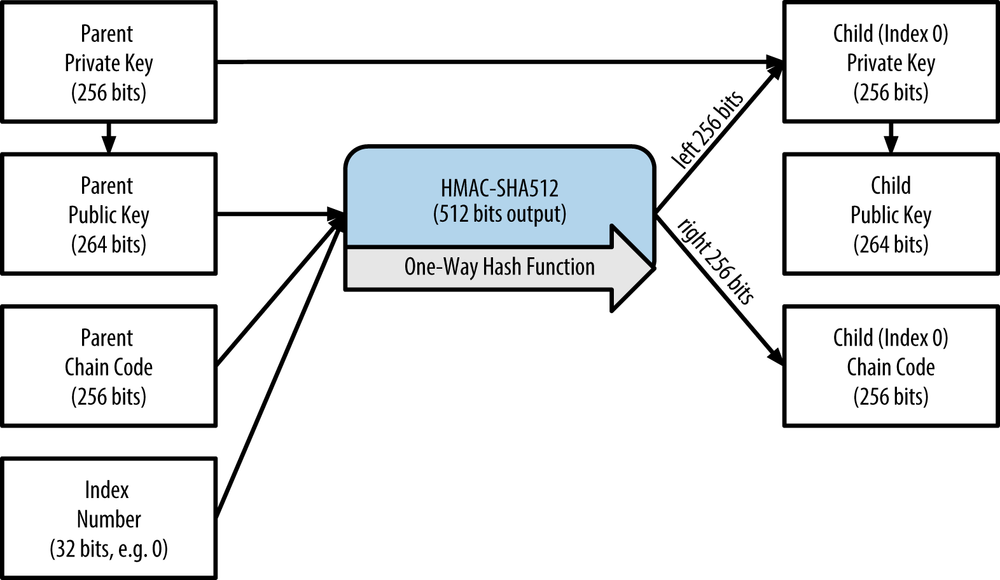
\includegraphics[scale = 0.4]{Images/bip32.png}
	\captionof{figure}{BIP32's unhardened derivation, source: \cite{RefWork:7}.}
	\label{fig:bip32}
\end{center}
Now, imagine an attacker is given a valid signature $(K, s)$ for public key $Q_P$ and message $m$. Relying on the previous relation, he is able to forge a valid signature for public key $Q_C$ and for the same message $m$ as $(K, s + \text{hash}(K \ || \ m)f)$. Indeed we have:
$$(s + \text{hash}(K \ || \ m)f)G = sG + \text{hash}(K \ || \ m)fG = $$
$$= K + \text{hash}(K \ || \ m)Q_P + \text{hash}(K \ || \ m)fG = K + \text{hash}(K \ || \ m)(Q_P + fG) = $$
$$ = K + \text{hash}(K \ || \ m)Q_C.$$
When substituting $sG$ with $K + \text{hash}(K \ || \ m)Q_P$ we relied on the fact that $(K, s)$ was a valid signature for public key $Q_P$ and message $m$. Notice that the attacker only needs a valid signature for the parent public key, the related public key and message, the parent chaincode and the child index.
\\
This is a particular case of the previously presented weakness, that now can be exploited since the relation between the two public keys is known. The hardened derivation also would prevent the forgery since, in place of the parent public key, the parent secret key is given as input to the hash function. To learn the relation between the two public keys, i.e. the offset, the forger would need to know also the parent private key. But this would mean that the attacker has direct access to all the funds secured by the subtree generated by the compromised parent node: the simple forgery is not anymore a concern.
\\
\\
The first problem we have to face is how to encode efficiently the point EC point in the signature, as we chose the $K$ option. Several possibilities exist:
\begin{enumerate}
	\item Encoding the full point through $x$ and $y$ coordinates, resulting in a 96 bytes signature (32 for each coordinate and another 32 for the integer $s$);
	\item Encoding the $x$ coordinate and use an additional byte to encode whether $y$ is odd or even, like for compressed public keys: this would result in a 65 bytes signature;
	\item Encoding only the $x$ coordinate making the point implicit, leading to a 64 bytes signature.
\end{enumerate}
In the BIP, the choice falls on the third option, since compactness is prioritized. However we cannot have ambiguity about the $y$ coordinate, so we need break the symmetry, i.e. we need to make the whole point $K$ implicit in its $x$ coordinate. Again, we have multiple possibilities:
\begin{enumerate}
	\item Select the $y$ coordinate in the lower half of the plane;
	\item Select the $y$ coordinate that is even;
	\item Select the $y$ coordinate that is a quadratic residue\footnote{It can be proved that the product of two numbers is a quadratic residue when either both or none of the factors are quadratic residues. Since we have that the two $y$ coordinates are one the negation of the other, and since -1 is not a quadratic residue when $p = 3 \ (\text{mod} \ 4)$ (as for secp256k1), we conclude that exactly one of the two roots is a quadratic residue. Notice that this choice for symmetry breaking prevents a real standardization: this formulation of Schnorr signature would not work for curves in which $p = 1 \ (\text{mod} \ 4)$.}.
\end{enumerate}
As directly stated in the BIP "the third option is slower at signing time but a bit faster to verify, as the quadratic residue of the $y$ coordinate can be computed directly for points represented in Jacobian coordinates. The two other options require a possibly expensive conversion to affine coordinates first. This would even be the case if the sign or oddness were explicitly coded". This is the statement with which the choice of the third option is justified.

\bigskip
\noindent
Hereinafter hash is the SHA-256 function and the elliptic curve on which everything is worked out is intended to be secp256k1. Now we pass to study the signing and verification algorithms. 

\begin{algorithm}
	\caption{Schnorr: signing algorithm}
	\label{alg:schnorr_sig}
	\begin{algorithmic}[1]
		\Procedure{schnorr\_sig}{$M, \ q$}
		\State $m \gets \text{hash}(\text{bytes}(M))$
		\State $k \gets \text{int}(\text{hash}(\text{bytes}(q) \ || \ m)) \ (\text{mod} \ n)$
		\State $K \gets kG$
		\If {$\text{jacobi}(y_K) \neq 1$}
		\State $k \gets n - k$
		\EndIf
		\State $e \gets \text{int}(\text{hash}(\text{bytes}(x_K) \ || \ \text{bytes}(qG) \ || \ m) \ (\text{mod} \ n)$
		\State $s \gets k + eq \ (\text{mod} \ n)$
		\State \textbf{return} $(\text{bytes}(x_K), \text{bytes}(s))$
		\EndProcedure
	\end{algorithmic}
\end{algorithm}

\noindent
We chose $k$ in such a way that it changes each time the signature algorithm is applied to a different message; indeed even with Schnorr the predictability of this secret value can be used to recover the private key. Given $(r_0, s_0)$ and $(r_1, s_1)$ we have, by definition of $s_i$:
$$k = s_0 - e_0q = s_1 - e_1q\ (\text{mod} \ n) \ \Longrightarrow \ q = (s_0 - s_1)(e_0 - e_1)^{-1} \ (\text{mod} \ n).$$

\bigskip

\begin{algorithm}
	\caption{Schnorr: verification algorithm}
	\label{alg:schnorr_ver}
	\begin{algorithmic}[1]
		\Procedure{schnorr\_ver}{$(r, s), M, Q$}
		\If {not $\text{isOnCurve}(Q)$ or $Q = \infty$}
		\State \textbf{return False}
		\EndIf 
		\State $r \gets \text{int}(r)$, $s \gets \text{int}(s)$
		\If {$r \notin [1, ..., p - 1]$ or $s \notin [1, ..., n - 1]$}
		\State \textbf{return False}
		\EndIf
		\State $m \gets \text{hash}(\text{bytes}(M))$
		\State $e \gets \text{int}(\text{hash}(\text{bytes}(r) \ || \ \text{bytes}(Q) \ || \ m) \ (\text{mod} \ n)$
		\State $K \gets sG - eQ$
		\If {$K = \infty$ or $\text{jacobi}(y_K) \neq 1$ or $x_K \neq r$}
		\State \textbf{return False} 
		\EndIf
		\State \textbf{return True}
		\EndProcedure	
	\end{algorithmic}
\end{algorithm}

\bigskip
\noindent
{\bf Proof of correctness}: Given the signature $(r, s)$, we need to prove that the elliptic curve point $K$, recoverable from the integer $r$, equals $sG - eQ$. But by definition of $s$ and by definition of public key, we have:
$$sG - eQ = (k + eq)G - eqG = kG = K.$$ 
\ \ \ \ \ \ \ \ \ \ \ \ \ \ \ \ \ \ \ \ \ \ \ \ \ \ \ \ \ \ \ \ \ \ \ \ \ \ \ \ \ \ \ \ \ \ \ \ \ \ \ \ \ \ \ \ \ \ \ \ \ \ \ \ \ \ \ \ \ \ \ \ \ \ \ \ \ \ \ \ \ \ \ \ \ \ \ \ \ \ \ \ \ \ \ \ \ \ \ \ \ \ \ \ \ \ \ \ \ \ \ \ \ \ \ \ \ \ \ \ $\square$

\bigskip
\noindent
{\bf Batch verification}: it is pretty common for a system to verify a large number of signatures, particularly now with crypto-currency widespread adoption. Thus, faster validation for a batch of signatures traduces in efficiency enhancements.
\\
When validating a signature in the formulation that we chose, the most expensive operations are the two elliptic curve scalar multiplications involved. Using the $(K, s)$ representation, we can verify the signature doing the hash operation first, and then perform elliptic curve operations. This is the key ingredient that allows to introduce batch validation.

\bigskip
\noindent
We established that a signature $(K, s)$ is valid if $K = sG - \text{hash}(K \ || \ Q \ || \ m)Q$. 
Therefore, a couple of valid signatures will verify:
$$K_0 + K_1 = s_0G - \text{hash}(K_0 \ || \ Q_0 \ || \ m_0)Q_0 + s_1G - \text{hash}(K_1 \ || \ Q_1 \ || \ m_1)Q_1 \Longrightarrow
$$
$$K_0 + K_1 = (s_0 + s_1)G - \text{hash}(K_0 \ || \ Q_0 \ || \ m_0)Q_0 - \text{hash}(K_1 \ || \ Q_1 \ || \ m_1)Q_1.$$
We are able to factorize multiplication by G summing all the $s$ values of the signatures: this approach reduces the number of scalar multiplication to one per signature, plus one for the aggregated $s$. Sadly, this is not secure at all: an attacker can produce a set of signatures that cancel each others. This could be a problem if the signatures are invalid. The attacker would convince the network that they are valid thanks to the batch validation that would succeed. There is also a simpler example that could help clarifying why this construction is not secure: imagine we have a set $(K_i, s_i), \ i \in \{1, ..., n\}$ of valid signatures. Obviously the naive batch validation would succeed. However it would be possible to switch the terms between the signatures, invalidating them all: nonetheless, the batch validation would still succeed. To work around this, we will introduce a random factor per signature. Not knowing the random factor for each of his signatures, the attacker is now unable to have them cancel each others:
$$a_0K_0 + a_1K_1 = (a_0s_0 + a_1s_1)G - a_0\text{hash}(K_0 \ || \ Q_0 \ || \ m_0)Q_0 - a_1\text{hash}(K_1 \ || \ Q_1 \ || \ m_1)Q_1.$$
Usually it is possible to rely on another trick at this point, namely we can write:
$$a_0K_0 + a_1K_1 = (a_0 - a_1)K_0 + a_1(K_0 + K_1)$$
By keeping a sorted list of points and factors, we could recursively pick the two largest values of $a$ and associated points, do the above mentioned transformation, and reinsert the two new factors and associated points in the list. Every time $a_0 - a_1$ is zero, a point can be removed from the list.
Doing so could lead to less scalar multiplication in the end; obviously, this would come at the cost of having way more point additions to do, but the more $a$ values you have, the easier it becomes to find two that cancel each others, and the more multiplications you save. This quickly becomes profitable with the number of signatures.
\\
However, this approach is not feasible in Bitcoin. This is linked to the fact that batch validation is made on a block basis, meaning that we would have some thousands of signatures. But the $a$ values are generated pseudo-randomly in $[1, ..., n - 1]$, where $n$ is the order of the curve. This number is around $2^{256}$, so that it would be very unlikely to end up with two factors that cancel out.

\bigskip
\noindent
Algorithm \ref{alg:schnorr_batch} presents the batch verification for a number $u$ of signatures $(r_1, s_1), ..., (r_u, s_u)$, associated to the messages $M_1, ..., M_u$ and to public keys $Q_1, ..., Q_u$.
\\
We remark the fact that the algorithm, taken from the BIP, is constructed to work on secp256k1, as clearly shown by the $14^{th}$ step, where we can see the defining equation. However it can be easily extended to other curves satisfying the relation $p = 3 \ (\text{mod} \ 4)$: this property is used in the $15^{th}$ step, that we try here to clarify. The $y$ coordinates are the square roots of $c$ and can be computed as $y = \pm c^{\frac{p + 1}{4}}$, if they exist, due to a lemma by Lagrange\footnote{\url{https://en.wikipedia.org/wiki/Quadratic\_residue\#Prime\_or\_prime\_power\_modulus}.}, applicable when $p \equiv 3 \ (\text{mod} \ 4)$. Euler's criterion tells us that, given an odd prime $p$ and an integer $c$ coprime to $p$, we have $c^{\frac{p - 1}{2}} = \pm 1 \ (\text{mod} \ p)$, depending whether $c$ is a quadratic residue or not. The same criterion applied to $y$ yields to $y^{\frac{p - 1}{2}} \ (\text{mod} \ p) = \pm c^{\frac{p + 1}{4}\frac{p - 1}{2}} \ (\text{mod} \ p) = \pm (c^{\frac{p - 1}{2}})^{\frac{p + 1}{4}} \ (\text{mod} \ p) = \pm 1^{\frac{p + 1}{4}} \ (\text{mod} \ p) = \pm 1 \ (\text{mod} \ p)$. Therefore, $y = c^{\frac{p + 1}{4}} \ (\text{mod} \ p)$ is a quadratic residue, while $-y \ (\text{mod} \ p)$ is not: this approach is thus used to comply with the chosen symmetry breaking method.

\begin{algorithm}
	\caption{Schnorr: batch verification algorithm}
	\label{alg:schnorr_batch}
	\begin{algorithmic}[1]
		\Procedure{schnorr\_batch}{$u, \{(r_1, s_1), ..., (r_u, s_u)\}, \{M_1, ..., M_u\}, \{Q_1, ..., Q_u\}$}
		\State $RHS \gets \infty$
		\State $mult \gets 0$
		\For {$i \gets 1,u$}
		\If {not isOnCurve$(Q_i)$ or $Q_i = \infty$}
		\State \textbf{return False}
		\EndIf
		\State $r_i \gets \text{int}(r_i)$, $s_i \gets \text{int}(s_i)$
		\If {$r_i \notin [1, ..., p - 1]$ or $s_i \notin [1, ..., n - 1]$}
		\State \textbf{return False}
		\EndIf
		\State $m_i \gets \text{hash}(M_i)$
		\State $e_i \gets \text{int}(\text{hash}(\text{bytes}(r_i) \ || \ \text{bytes}(Q_i) \ || \ m_i) \ (\text{mod} \ n)$
		\State $c \gets r^3 + 7 \ (\text{mod} \ p)$
		\State $y \gets c^{\frac{p + 1}{4}}$
		\If {$y^2 \neq c$}
		\State \textbf{return False}
		\EndIf
		\State $K_i \gets (r_i, y)$
		\If {$i \neq 1$}
		\State  $a_i \xleftarrow{\text{\$}} [1, ..., n - 1]$ 
		\Else
		\State $a_i \gets 1$
		\EndIf
		\State $mult \gets mult + a_is_i$
		\State $RHS \gets a_iK_i + (a_ie_i)Q_i$
		\EndFor
		\If {$multG \neq RHS$}
		\State \textbf{return False}
		\EndIf
		\State \textbf{return True}
		\EndProcedure	
	\end{algorithmic}
\end{algorithm}
\chapter{Schnorr's applications}
\label{chpr:application}
In this chapter we will present some of the applications that Schnorr would make deployable in Bitcoin: we will study improved multi and threshold signature schemes and we will see the construction called adaptor signature, that allows the development of the so called \textit{scriptless scripts}, affecting considerably privacy and efficiency in cross-chain atomic swaps and in the Lightning Network.
\\
In case the reader is not familiar with Bitcoin's inner working, we recommend the reading of Appendix \ref{app:A}.

\bigskip

\section{Multi-signature: MuSig ($\mu \Sigma$)}
\label{musig}
Usually Schnorr is presented with an implicit multi-signature scheme: given $n$ users that want to sign a single message $m$, they can sign it on their own, the final signature being the sum of the so called partial signatures. This signature can then be verified against the sum of the public keys.
\\
Let's study this scheme through an example: Alice and Bob have key pairs $\{q_A, Q_A\}$ and $\{q_B, Q_B\}$, respectively. If both participants are honest, they will proceed as follows: they exchange their public keys, computing the aggregated one $Q = Q_A + Q_B$. Then each one of them calculate as usual the public nonces $K_A$ and $K_B$, defining the joint nonce as $K = K_A + K_B$. The signature would then be $(x_K, s)$, with $s = s_A + s_B = k_A + \text{hash}(x_K \ || \ Q \ || \ m)q_A + k_B + \text{hash}(x_K \ || \ Q \ || \ m)q_B \ (\text{mod} \ n)= (k_A + k_B) + \text{hash}(x_K \ || \ Q \ || \ m)(q_A + q_B) \ (\text{mod} \ n)$. Looking exactly as a single user signature, the verification procedure would follow Algorithm \ref{alg:schnorr_ver}.
\\
This sounds great, except for the fact that it is a completely insecure scheme: we assumed that both the participants were honest, a deadly hypothesis for every cryptosystem. Imagine that it is Bob that wants to cheat. He could simply says that his public key is $Q_B' = Q_B - Q_A$. Then, if someone sends money to the address associated to $Q = Q_A + Q_B' = Q_A + Q_B - Q_A = Q_B$, clearly Bob can control the funds by himself, being in possess of the associated private key.
\\
This kind of attack is called rogue key attack and is a serious concern for multi-signature schemes: given $n$ participants, a subset of $1 \leq t < n$ dishonest signers use public keys that are functions of the public keys of honest signers, allowing them to forge a signature without the aid of the honest signers for the whole set of public keys. There are certain ways to prevent such an attack: for example by ensuring that the participants own the private keys associated with the alleged public keys (now it is not possible for Bob to cheat, since it would imply breaking the ECDLP), a setting that takes the name of KOSK (knowledge of secret key). 

\bigskip
\noindent
In this section we will present a provably secure multi-signature scheme of the type $n$-of-$n$. But before delving into its technicalities, it could be better to stop and talk a little about how changes are introduced in Bitcoin: deploying innovations in Bitcoin is a long procedure, due to its decentralized consensus protocol. Since it could require years to take a new feature to it, we should think about properties that would enhance Bitcoin in the long term. Today Bitcoin is missing some important properties in order to be a good method of payment: it is missing both fungibility and privacy. It is missing fungibility due to the fact that it is missing privacy: Bitcoin is pseudonymous, not anonymous, in the sense that an address is not directly linked to a physical person, but every single transaction is on the public  ledger open to (possibly) every node in the network. Low privacy means that bitcoins, not being interchangeable, could be treated differently: think about the bitcoins possessed by the creator of Bitcoin, Satoshi Nakamoto, and not moved since the creation of Bitcoin. Obviously they have not the same appeal of newly minted coins.
\\
Fortunately enough, the lack of some properties is not everlasting: for such a reason, when introducing a new feature in Bitcoin we should try to fix these problems. So, we will give now a look to some properties that, in a long term view, a new multi-signature scheme should possess:
\begin{enumerate}
	\item Accountability: this property refers to $m$-of-$n$ multi-signature schemes (also referred to as threshold schemes) and deals with the fact that for the participants of the scheme should be possible to know who signed and to show to others that they have not;
	\item Usability: the ease of use is important. If an interactive scheme requires a huge number of rounds, it won't be used by anyone;
	\item Privacy: third parties should learn as little about the policy of the scheme as possible (particular kind of policies could identify your transactions, leading to various problems, like censorship by miners).
\end{enumerate}

\bigskip
\noindent
After this brief digression, we are ready to present the MuSig scheme \cite{RefWork:11}. MuSig is an interactive (meaning that the scheme comprehends different rounds of communication between the participants) multi-signature scheme, based on the Schnorr signature. MuSig has some very attractive properties, namely:
\begin{itemize}
	\item The size of the signature is equal to the single user case;
	\item It is provably secure in the plain public key model\footnote{The signers are only required to have a public key: they do not have to prove ownership of it, i.e. knowledge of the associated private key.}.
\end{itemize}
These properties, although being appealing, are not original: MuSig shares them with other schemes, in particular with the Bellare-Neven (BN) scheme \cite{RefWork:10}. The novelty introduced by the authors is that they recovered key aggregation, meaning that to the scheme can be associated a unique joint public key, leading to a verification algorithm that is equal to the single user case: the multi-signature can be verified with respect to a single aggregated public key, leading to greater privacy since for third parties the multi-signature policy is completely hidden.
\\
The Bellare-Neven scheme prevents rogue key attacks relying on a particular algorithm to compute the partial signatures, avoiding a trusted setup: each participant $i \in \{1, ..., n\}$ with key pair $\{q_i, Q_i\}$ computes $s_i = k_i + c_iq_i, \ c_i = \text{hash}(\langle L \rangle\ || \ K \ || \ Q_i \ || \ m)$, where $K = \sum_{i = 1}^{n}K_i$ is the aggregated public nonce, $m$ is the message to be signed and $\langle L \rangle$ is a unique encoding of the multiset of public keys $L = \{Q_1, Q_2, ..., Q_n\}$, e.g. ordered lexicographically. The signature is $(K, s)$, where $s = \sum_{i = 1}^{n}s_i$, and the verification equation is: $sG = K + \sum_{i = 1}^{n}c_iQ_i$. We can notice that a validator needs the whole set of public keys in order to check the signature. 
\\
MuSig can be thought as a variant of BN that recovers key aggregation. The setting in which the two schemes are defined is the same: both can be proven to be secure in the plain public key model under the discrete logarithm assumption\footnote{The discrete logarithm assumption requires the DL to be hard on the selected group. This means that if the DL is hard, then the scheme is secure.}, modelling the hash functions involved as a public random oracle.
\\
Security is to be intended in the sense that it is infeasible for an adversary to forge multi-signatures involving at least an honest participant, that is: the adversary is not able to produce on its own a signature valid for the set of public keys containing the one of the honest signer.
\\
We stress the fact that, from the applicative point of view, key aggregation is a fundamental property: if the scheme is usable (few interaction rounds), then we get for free privacy and accountability (MuSig is an $n$-of-$n$ scheme, so that it is possible to generate a valid signature only if all the participants agree). Indeed, thanks to key aggregation, verifiers will only see an aggregated public key: they would not even know that it is indeed aggregate, since it is indistinguishable from a normal public key. This is also important from the point of view of efficiency: in Bitcoin every single node has the possibility of validating each transaction, meaning that verification efficiency and signature size are very important, more than the timing of the signing algorithm. This is why, although there are multi-signature schemes with fewer interaction rounds, we present here MuSig: the benefits of key aggregation are improved bandwidth (no need for communication of multiple public keys), privacy (aggregated public key indistinguishable from a normal one) and validation efficiency (as efficient as a normal Schnorr's verification).
\\
Moreover if the aggregated public key is not given to the verifier, it is still possible to recover it just from the set of public keys of the participant, without interaction with the signers.

\bigskip
\noindent
The plain public key setting plays a crucial role when trying to enable multi-signatures across multiple inputs of a Bitcoin transaction, resulting in a unique signature per transaction.  In case the transaction spends inputs from different owners, they will obviously need to collaborate to produce the multi-signature. Such a construction would reduce further the traffic on-chain, resulting in a benefit for all the network participants. Such a change would require the introduction of new opcodes in the Bitcoin scripting language, but this can be done via a soft fork (i.e. in a backward compatible way). To see why security in the plain public key model is fundamental to enable cross-input multi-signature, think about an attacker that identifies some outputs he wants to steal, corresponding to a set $\{Q_1, Q_2, ..., Q_{n - t}\}$ of public keys. He could try to identify another set of keys $\{Q_{n - t + 1}, ..., Q_n\}$ such that he can sign for the aggregated public key. He would be able to steal the coins just by sending a small amount of his own money to outputs corresponding to the keys he found and finally creating a transaction referencing the outputs he wants to steal and the newly created outputs in his possession: by construction he is able to forge a signature on his own for this transaction. But the plain public key model defends exactly against such a situation, since the game is won by the adversary if he is able to forge a signature over a set of keys that includes at least one key not in possession of the attacker. 
\\
In the setting of signature aggregation on a transaction basis, it is possible to resort to signature schemes different from MuSig (in particular the older and more reviewed BN scheme), since all the public keys involved are public.
\\
Up to now we have talked about cross-input aggregation, that would reduce the number of signatures to one per transaction. Is it possible to go further? For example, is it possible to obtain a single signature on a block basis? Unfortunately it is not possible through MuSig, since the scheme is interactive: this obviously prevents aggregation on a block level. However the discussion would not be fair if we would not point out that changing signature scheme would allow aggregation on a block basis: for example the BLS signature scheme (\cite{RefWork:15}, \cite{RefWork:16}) is non interactive when it comes to aggregation. This would enable a single signature per block. However, although there is interest around BLS signatures, it is underpinned by different cryptographic hypothesis than ECDSA and Schnorr. For this reason the Bitcoin community is working towards the implementation of Schnorr.

\bigskip
\noindent
Now we can finally look at the inner working of the scheme: it is parameterized by the cyclic group $\mathbb{G}$ (a subgroup of $E(\mathbb{F}_p)$), its order $n$, a generator of the group $G$ and three hash functions $\text{hash}_{com}, \ \text{hash}_{agg}$ and $\text{hash}_{sign}$: $\{0, 1\}^* \to \{0, 1\}^{L_n}$. The bit length of the order $n$ is denoted by $L_n$ and assumed to be a security parameter. The key generation algorithm is not presented: we assume each participant $i \in \{1, ..., m\}$ is in possession of a proper key pair $\{q_i, Q_i\}$. The signing algorithm is presented by Algorithm \ref{alg:musig_sig}. In the following $\langle L \rangle$ denotes a unique encoding of the multiset of public keys and the indices used in the signing algorithm are local references to the other cosigners. The algorithm is split in interactive rounds according to the \textbf{send} and \textbf{upon reception of} commands. Verification occurs following the single signature Schnorr verification Algorithm \ref{alg:schnorr_ver}.

\bigskip

\begin{algorithm}
	\caption{MuSig: signing algorithm}
	\label{alg:musig_sig}
	\begin{algorithmic}[1]
		\Procedure{MuSig\_sig}{$M, q_1, \{Q_2, ..., Q_m\}$}
		\State $m \gets \text{hash}(M)$
		\State $\langle L \rangle \gets \{q_1G, Q_2, ..., Q_m\}$
		\For {$i \gets 1, m$}
		\State $a_i \gets \text{int}(\text{hash}_{agg}(\langle L \rangle \ || \ \text{bytes}(Q_i)))$
		\EndFor
		\State $Q \gets \sum_{i = 1}^{m}a_iQ_i$
		\State $k_1 \xleftarrow{\text{\$}} \{1, ..., n - 1\}$
		\State $K_1 \gets k_1G, \ t_1 \gets \text{hash}_{comm}(\text{bytes}(K_1))$
		\State \textbf{send} $t_1$
		\State \textbf{upon reception of} $t_2, ..., t_m$ \textbf{send} $K_1$
		\State \textbf{upon reception of} $K_2, ..., K_m$ \textbf{do}
		\State $\ \ \ \ \ $ \textbf{for} $i \gets 2, m$ \textbf{do}
		\State $\ \ \ \ \ \ \ \ \ \ $ \textbf{if} $t_i \neq \text{hash}_{comm}(\text{bytes}(K_i))$ \textbf{do}
		\State $\ \ \ \ \ \ \ \ \ \ \ \ \ \ \ $ \textbf{abort}
		\State $\ \ \ \ \ \ \ \ \ \ $ \textbf{end if}
		\State $\ \ \ \ \ $ \textbf{end for} 
		\State $K \gets \sum_{i = 1}^{m}K_i$
		\If {$\text{jacobi}(y_K) \neq 1$}
		\State $k_1 \gets n - k_1$
		\EndIf
		\State $c \gets \text{int}(\text{hash}_{sig}(\text{bytes}(x_K) \ || \ \text{bytes}(Q) \ || \ m))$
		\State $s_1 \gets k_1\ + ca_1q_1 \ (\text{mod} \ n)$
		\State \textbf{send} $s_1$
		\State \textbf{upon reception of} $s_2, ..., s_m$ \textbf{do}
		\State $s \gets \sum_{i = 1}^{m}s_i \ (\text{mod} \ n)$
		\State \textbf{return} $(x_K, s)$
		\EndProcedure
	\end{algorithmic}
\end{algorithm}

\bigskip
\noindent
As usual, here follows the proof of the correctness.
\\
{\bf Proof}: Loosely speaking, we have to prove that $sG = K + cQ$.
\\
$$sG = \left(\sum_{i = 1}^{m} s_i\right)G = \left(\sum_{i = 1}^{m}(k_i + ca_iq_i)\right)G = \sum_{i = 1}^{m}(k_iG + ca_iq_iG) =$$
$$= \sum_{i = 1}^{m}k_iG + \sum_{i = 1}^{n} ca_iq_iG = \sum_{i = 1}^{m}K_i + c\sum_{i  = 1}^{m}a_iQ_i = K + cQ.$$
\ \ \ \ \ \ \ \ \ \ \ \ \ \ \ \ \ \ \ \ \ \ \ \ \ \ \ \ \ \ \ \ \ \ \ \ \ \ \ \ \ \ \ \ \ \ \ \ \ \ \ \ \ \ \ \ \ \ \ \ \ \ \ \ \ \ \ \ \ \ \ \ \ \ \ \ \ \ \ \ \ \ \ \ \ \ \ \ \ \ \ \ \ \ \ \ \ \ \ \ \ \ \ \ \ \ \ \ \ \ \ \ \ \ \ \ \ $\square$

\bigskip
\noindent
For the security proof of the scheme we refer to the original article \cite{RefWork:11}. 
\\
Dealing with ECDSA and Schnorr in Chapter \ref{chpr:dss}, we have seen that in the single user setting there was the possibility to derandomize the signature algorithm without loss of security, by generating the random nonce $k$ through a deterministic function. This is done since pseudo random generation is one of the major sources of problems in cryptography. This is not anymore suggested in the multi-user setting: it is necessary to ensure to use different unpredictable values when the other signers change their $K$ values in repeated signing attempts, otherwise secret key recovery would be possible. 
\\
Here follows an example taken directly from \cite{RefWork:11}: assume Alice and Bob have key pairs $\{q_A, Q_A\}$ and $\{q_B, Q_B\}$, respectively. They want to jointly produce a signature. Alice generates $k_A$ and sends $K_A = k_AG$ to Bob. In a first attempt, Bob responds with $K_B$. Alice then computes:
$$K = K_A + K_B,$$
$$c = \text{hash}_{sig}(x_K \ || \ Q \ || \ m),$$
$$s_A = k_A + ca_Aq_A \ (\text{mod} \ n),$$
and sends $s_A$ to Bob. Bob is trying to cheat on Alice, and decides not to produce a valid $s_B$, and thus the protocol fails. A new signing attempt takes place, and Alice again sends the same $K_A$. Bob responds with $K_B' \neq K_B$. Alice then computes $c' = \text{hash}_{sig}(x_{K_A + K_B'} \ || \ Q \ || \ m)$ and $s_A' = k_A + c'a_Aq_A \ (\text{mod} \ n)$ and sends $s_A'$ to Bob. Now Bob is able to derive Alice's private key:
$$s_A - s_A' = (c - c')a_Aq_A \ (\text{mod} \ n) \ \Longrightarrow \ q_A = (c - c')^{-1}a_A^{-1}(s_A - s_A') \ (\text{mod} \ n).$$
To avoid this problem, each signer must ensure that whenever any $K$ value sent by other cosigners or the message $m$ changes, his $k_i$ changes as well. 

\bigskip

\bigskip

\section{Threshold signature}
\label{threshold}
With the name threshold signatures we refer to policies of the kind $m$-of-$n$, where it is necessary that at least $m$ participants of the scheme decide to collaborate to produce a valid signature. This kind of policy is very popular in Bitcoin, since it is flexible and has many applications: for example, a single user could use such a policy to improve security, storing the keys on different machines, at the same time defeating the risk of loss of some keys. 
\\
In this section we will study a provably secure Schnorr based threshold scheme. For the security proof we refer to \cite{RefWork:14}. The scheme is constructed on top of the Pedersen Verifiable Secret Sharing Scheme (VSS scheme) and Pedersen's multi-party protocol to generate a random shared secret, hence we start presenting these two schemes.

\bigskip

\subsection{Verifiable secret sharing scheme}
\label{subsec:1}
Hereinafter, we will refer to threshold signature schemes as $t$-of-$m$ schemes in order to avoid confusion in the notation.
\\
Typically, in a $t$-of-$m$ secret sharing scheme, a trusted dealer distributes a secret $s$ to $m$ players $P_1, ..., P_m$ in such a way that any subgroup of at least $t$ members can recover the secret, while any subgroup of cardinality strictly less than $t$ learns nothing about it. A verifiable secret sharing scheme moreover prevents the dealer from cheating, since each participant can verify that his share of the secret is consistent with the others. The novelty introduced by Pedersen is that his scheme is non-interactive in the verification and does not require trust between the parties involved. Still there is a central dealer, a figure we would like to get rid of: this will be done through the second protocol that will be presented in Section \ref{subsec:2}. Here follows the VSS scheme proposed by Pedersen.

\bigskip
\noindent
Fix an elliptic curve over a prime finite field $E(\mathbb{F}_p)$, characterized by the EC domain parameters $T = (a, b, p, G, n, h)$ and fix another generator $H$ of the same cyclic group generated by $G$. We require that these two generators are \textit{nothing up my sleeves} (NUMS), meaning that we do not know the discrete logarithm of one with respect to the other, and vice versa.
\\
Assume that the dealer has a secret value $s \in \mathbb{Z}_n$ and a number $s' \in \mathbb{Z}_n$ generated at random. He commits\footnote{A commitment scheme is a cryptographic primitive used to commit to some secret data without revealing anything about it. Commitment schemes are designed so that it is unfeasible to change the secret: when revealed in a second moment, we have probabilistic assurance that it is the real committed value. A typical example of commitment scheme is a collision resistant hash function, e.g. SHA-256.} to the couple $(s, s')$ through the so called Pedersen commitment $C_0 = sG + s'H$. The NUMS property is needed to prevent the person who commits from lying about the values he committed to. Assume indeed that the dealer knows the discrete logarithm of $H$ with respect to $G$: $H = r_HG$. In this case he could write: $C_0 = sG + s'H = (s + s'r_H)G = (s \pm ar_H + s'r_H)G = (s - ar_H)G + (s'r_H + ar_H)G = (s - ar_H)G + (s' + a)H, \ \forall a \in \mathbb{Z}_n$.  As the calculations clearly show, knowing the DL the dealer could commit so the couple $(s, s')$ but later reveal $(s - ar_H, s' + a)$.
\\
After having broadcast the commitment, the secret $s$ can be shared among $P_1, ..., P_m$ through the following protocol:

\bigskip
\noindent
{\bf The dealer}:
\begin{enumerate}
	\item Chooses a couple of random polynomials of degree $t - 1$: 
	$$f(u) = s + f_1u + ... + f_{t - 1}u^{t - 1} \ (\text{mod} \ n),$$
	$$f'(u) = s' + f'_1u + ... + f'_{t - 1}u^{t - 1} \ (\text{mod} \ n),$$
	where $s \ \text{and} \ s'$ are the committed values, while $f_i, f'_i \in \mathbb{Z}_n$ are randomly chosen for every $i \in \{1, ..., t - 1\}$;
	\item Computes $(s_i, s'_i) = (f(i), f'(i))$ for $i \in \{1, ..., m\}$;
	\item Sends secretly $(s_i, s'_i)$ to $P_i, \forall i \in \{1, ..., m\}$;
	\item Broadcasts the values $C_j = f_jG + f'_jH, \ \forall j \in \{1, ..., t - 1\}$.
\end{enumerate}

\bigskip

\noindent
{\bf Each participant $P_i$}:
\begin{enumerate}
	\item Verifies the consistency of its share of the secret as:
	$$s_iG + s'_iH = \sum_{j = 0}^{t - 1}i^jC_j.$$
	If this check fails, she broadcasts a compliant against the dealer;
	\item For each compliant from a player $i$, the dealer defends himself by broadcasting the values $(s_i, s'_i) = (f(i), f'(i))$ that satisfy the checking equation at point 1;
	\item Aborts the protocol if:
	\begin{itemize}
		\item The dealer received more than $t$ compliants;
		\item He answered to a compliant with values that violate again the checking equation.
	\end{itemize}
\end{enumerate}
Pedersen proved that any coalition of less than $t$ players cannot get any information about the shared secret, provided that the discrete logarithm in $E(\mathbb{F}_p)$ is hard\footnote{This is important since we are not adding cryptographic assumptions.}. For the proof we refer to the original paper \cite{RefWork:13}. Although we do not look at the proof, it may still be of interest to check why the verification procedure at step 1 should succeed:
$$s_iG+ s'_iH = f(i)G + f'(i)H = \sum_{j = 0}^{t- 1}f_ji^jG + \sum_{j = 0}^{t - 1}f'_ji^jH =$$
$$= \sum_{j = 0}^{t - 1}i^j(f_jG + f'_jH)= \sum_{j = 0}^{t - 1}i^jC_j.$$
We used the convention that $f_0 = s$ and $f'_0 = s'$. Remembering that $C_0$ commits to the secret and that the other $C_j$ commits to the polynomials, we have the assurance that the dealer is not cheating. Indeed there is one and only one polynomial over $\mathbb{Z}_n$ of degree at most $t - 1$ satisfying $f(i) = s_i$, respectively $f'(i) = s'_i$, for $t$ values of $i$. 
\\
This is also the key property that allows the reconstruction of the secret value from any group $\mathcal{P}$ of $t$ participants. Indeed the members in $\mathcal{P}$ can recover the polynomial $f$ through the Lagrange's interpolation formula, that given a set of $t$ points $(i, s_i = f(i))$ returns the lowest degree polynomial (in this case a $t - 1$ degree polynomial) interpolating the given points:
$$f(u) = \sum_{i \in \mathcal{P}}f(i)\omega_i(u) \ (\text{mod} \ n), \ \text{where} \ \omega_i(u) = \prod_{j \in \mathcal{P}, \ j \neq i}\frac{u - j}{i - j} \ (\text{mod} \ n).$$
Since it holds that $s = f(0)$ by definition, the group $\mathcal{P}$ can directly reconstruct the secret as:
$$s = f(0) = \sum_{i \in \mathcal{P}}f(i)\omega_i \ (\text{mod} \ n),  \ \text{where} \ \omega_i = \omega_i(0) = \prod_{j \in \mathcal{P}, \ j \neq i}\frac{j}{j - i} \ (\text{mod} \ n).$$

\bigskip

\subsection{Protocol for the generation of a random shared secret}
\label{subsec:2}
As we pointed out before, we would like to get rid of the figure of the dealer, so that it is possible to generate a key pair between distrustful parties without his intervention. The key generation phase of the signature scheme generates a random shared secret key in a distributed way according to the following protocol:
\\
\\
{\bf Each participant $P_i$}:
\begin{enumerate}
	\item Chooses $r_i, r'_i \in \mathbb{Z}_n$ at random and verifiably shares $(r_i, r'_i)$ acting as the dealer according to the Pedersen's VSS scheme described above. Let the sharing polynomials of participant $i$ be $f_i(u) = \sum_{j = 0}^{t - 1}a_{ij}u^j \ (\text{mod} \ n)$, $f'_i(u) = \sum_{j= 0}^{t - 1}a'_{ij}u^j \ (\text{mod} \ n)$, where $a_{i0} = r_i$ and $a'_{i0} = r'_i$. The public commitments are $C_{ik} = a_{ik}G + a'_{ik}H$ for $k \in \{0, ..., t - 1\}$;
	\item Sets $H_0 = \{P_j \ | \ P_j \ \text{is not detected to be cheating at step 1}\}$. The distributed secret value $r$ is equal to $\sum_{i \in H_0}r_i \ (\text{mod} \ n)$ (but nobody can compute it on its own). Each participant $P_i$ sets his share of the secret at $s_i= \sum_{j \in H_0}f_j(i) \ (\text{mod} \ n)$ and sets the value $s'_i = \sum_{j \in H_0}f'_j(i) \ (\text{mod} \ n)$ (the share of the secret is simply equal to the sum of the partial shares received from honest participants);
	\item Each player in $H_0$ broadcasts $R_i = r_iG$ via Feldman's VSS scheme:
	\begin{enumerate}
		\item Each player $P_i$ in $H_0$ broadcasts $A_{ik} = a_{ik}G$ for $k \in \{0, ..., t - 1\}$;
		\item Each player $P_j$ verifies the values broadcast by the other players in $H_0$, i.e. for each $P_i \in H_0$, $P_j$ checks that:
		$$f_i(j)G = \sum_{k = 0}^{t - 1} j^kA_{ik}.$$
		If the check fails for an index $i$, $P_j$ complaints against $P_i$ broadcasting the values $(f_i(j), f'_i(j))$ that satisfy the checking equation of the Pedersen's VSS scheme  but not the one at point (b);
		\item For players $P_i$ who received at least one valid complaint, the other players run the reconstruction phase of Pedersen's VSS scheme to compute $r_i$, $f_i(u)$ and $A_{ik}$ for $k \in \{0, ..., t - 1\}$. All participants in $H_0$ set $R_i = r_iG$. 
	\end{enumerate} 
\end{enumerate}
After the execution of the protocol the following equations hold:
$$R = \sum_{i \in H_0} R_i = \sum_{i \in H_0}r_iG = \sum_{i \in H_0}A_{i0} = rG,$$
$$f(u) = \sum_{i \in H_0} f_i(u) = r + a_1u + ... + a_{t - 1}u^{t - 1} \ (\text{mod} \ n), \ \text{where} \ a_i = \sum_{j \in H_0}a_{ji} \ (\text{mod} \ n),$$
$$f(i) = s_i.$$
We introduce the following notation: 
$$(s_1, ..., s_n) \xleftrightarrow{\text{(t, m)}} (r|R, a_iG, H_0), \ i \in \{0, ..., t - 1\}.$$
It means that $s_j$ is the share of secret key $r$ belonging to $P_j$ for $j \in H_0$. The values $a_iG$
are the public commitments of the sharing polynomial and $\{r, R\}$ is the key pair that can be reconstructed by any subgroup of $H_0$ composed of at least $t$ participants: this can be done via Lagrange's interpolation formula, as described in Section \ref{subsec:1}.
\\
Before we pass to analyse the actual signature scheme, let's give a look at the checking equation at point (b) in the protocol and verify why it should work:
$$f_i(j)G = \sum_{k = 0}^{t - 1}a_{ik}j^kG = \sum_{k = 0}^{t - 1}j^kA_{ik}.$$

\bigskip

\subsection{Threshold signature scheme}
Now that we have defined the primitives on which it is built, we can finally discuss the protocol that implements the $t$-of-$m$ threshold signature scheme. It is important to understand that the participants do not simply recover the private key: this would allow anyone possessing it to sign on the behalf of every other participant in the scheme, even those that did not take part in the reconstruction procedure. Instead, as we will see, the approach consists in the generation of a partial signature through the share of secret key in possession of each user.

\bigskip
\noindent
{\bf Key generation}: All $m$ participants have to cooperate to generate a public key $Q$ and a share of the secret key for each participant $P_j$. This can be done relying on the protocol presented in Section \ref{subsec:2}. The output of the protocol is:
$$(\alpha_1, ..., \alpha_m) \xleftrightarrow{\text{(t, m)}} (q|Q, b_iG, H_0), \ i \in \{0, ..., t - 1\}.$$
The $\alpha$ values denote the secret key share belonging to $P_j$. They will be used to generate a partial signature for the key pair $\{q, Q\}$.
\\
\\
{\bf Signing algorithm}: Let $msg$ denote the message to be signed. Suppose that a subset $H_1 \subseteq H_0$ wants to issue a signature. The members of $H_1$ proceed as follows:
\begin{enumerate}
	\item If $|H_1| < t$, abort. Otherwise, the subset $H_1$ generates a random shared secret following again the protocol presented in Section \ref{subsec:2}. We denote the output as:
	$$(\beta_1, ..., \beta_m) \xleftrightarrow{\text{(t, m)}} (k|K, c_iG, H_2), \ i \in \{0, ..., t - 1\};$$
	\item If $\text{jacobi}(y_K) \neq 1$, then each player $i$ sets $\beta_i = n - \beta_i$;
	\item If $|H_2| < t$, aborts. Otherwise, each $P_i \in H_2$ reveals
	$$\gamma_i = \beta_i + e\alpha_i \ (\text{mod} \ n),$$
	where $e = \text{int}(\text{hash}(\text{bytes}(x_K) \ || \ \text{bytes}(Q) \ || \ msg))$.
	\item Each $P_i \in H_2$ verifies $\forall P_l \in H_2$:
	$$\gamma_lG = \begin{cases} K + \sum_{j = 1}^{t - 1} c_jl^jG + e\left(Q + \sum_{j = 1}^{t - 1}b_jl^jG\right), & \mbox{if } \text{jacobi}(y_K) = 1 \\ - K -\sum_{j = 1}^{t - 1} c_jl^jG + e\left(Q + \sum_{j = 1}^{t - 1}b_jl^jG\right), & \mbox{if } \text{jacobi}(y_K) \neq 1 \end{cases}$$
	Let $H_3 = \{P_j \ | \ P_j \ \text{not detected to be cheating at step 4}\}$.
	\item If $|H_3| < t$, abort. Otherwise each $P_i \in H_3$ selects an arbitrary subset $H_4 \subseteq H_3$ with $|H_4| = t$ and computes $\sigma$ satisfying $\sigma = k + eq \ (\text{mod} \ n)$, where:
	$$\sigma = \sum_{j \in H_4}\gamma_j\omega_j \ (\text{mod} \ n), \ \text{where} \ \omega_j = \prod_{h \in H_4, \ h \neq j}\frac{h}{h - j} \ (\text{mod} \ n).$$
	The signature is $(x_K, \sigma)$; it is verified as a simple Schnorr signature.
\end{enumerate}
This concludes the presentation of the protocol. Nonetheless there are some formulas that deserve greater attention.
\begin{itemize}
	\item Checking formula at point 4\footnote{The formula is checked in case $\text{jacobi}(y_K) = 1$; the other case is proved in a similar way.}: 
	$$\gamma_lG = (\beta_l + e\alpha_l)G = \beta_lG + e\alpha_lG = $$
	$$= \left(k + \sum_{j = 1}^{t - 1}c_jl^j\right)G + e\left(q + \sum_{j = 1}^{t - 1}b_jl^j\right)G =$$
	$$= K + \sum_{j = 1}^{t - 1}c_jl^jG + e\left(Q + \sum_{j = 1}^{t - 1}b_jl^jG\right).$$
	\item Formula used to compute $\sigma$: we defined $\gamma_i = \beta_i + e\alpha_i \ (\text{mod} \ n), \ \forall i \in H_2$. In particular the equation holds for every $i \in H_4$, with $|H_4| = t$. The $\alpha$ and $\beta$ values are defined to be the pointwise evaluation of the sharing polynomials created during the two iterations of the Pedersen protocol for the generation of a random shared secret, that we denote by $F_1(u)$ and $F_2(u)$. These polynomials have degree $t - 1$, so that we can define another polynomial of degree $t - 1$ as:
	$$F_3(u) = F_2(u) + eF_1(u) \ \Longrightarrow $$
	$$\Longrightarrow \ F_3(0) = F_2(0) + eF_1(0) \Longrightarrow $$
	$$\Longrightarrow \sigma := F_3(0) = k + eq \ (\text{mod} \ n).$$
	At this point we can apply the Lagrange's interpolation formula, since we know that $F_3(u)$ satisfies by construction $F_3(i) = \gamma_i$:
	$$F_3(u) = \sum_{j \in H_4}\gamma_j\omega_j(u) \ (\text{mod} \ n), \ \text{where} \ \omega_j(u) = \prod_{h \in H_4, \ h \neq j}\frac{u - h}{j -h} \ (\text{mod} \ n).$$
	Thus, $\sigma$ can be directly computed as:
	$$\sigma = F_3(0) = \sum_{j \in H_4}\gamma_j\omega_j \ (\text{mod} \ n), \ \text{where} \ \omega_j = \prod_{h \in H_4, \ h \neq j}\frac{h}{h - j} \ (\text{mod} \ n).$$
\end{itemize}
Notice that the scheme is robust, meaning that a corrupt signer who does not follow the protocol will be detected. The validity of the partial signatures computed at step 3 is immediately tested at step 4.

\bigskip

\bigskip
\noindent
The scheme presented is complex and cumbersome, but all the computations and interactions burden the participants who freely decided to rely on it. The Bitcoin blockchain would see a standard transaction with a single signature, indistinguishable from others. Nobody could tell that it required a threshold signature. This means that the protocol is highly private, but it comes with the downside of not being accountable, since the participants that do not sign cannot learn who instead did it. As usual, it is a matter of trade-offs: if accountability is desired, the naive ECDSA approach should be preferred (and will be available), otherwise users aiming at better privacy could rely on the presented Schnorr threshold scheme.

\bigskip

\bigskip

\section{Adaptor signature}
\label{adaptor}
Adaptor signatures are the building block for the so called \textit{scriptless script}, an innovative idea by Andrew Poelstra: the major aim is to introduce much more flexibility in systems lacking a scripting language (e.g. the Mimblewimble protocol discussed in \cite{MW1} and \cite{MW2}). However, it turns out that these kind of signatures have a couple of interesting applications also in Bitcoin, that we are going to explore.
\\
Adaptor signatures are based on Schnorr and leverage its linearity property. Therefore, introducing Schnorr in Bitcoin would allow the deployment of adaptor signatures for free. As we will see in the next two sections, this tool could affect significantly cross-chain atomic swaps and payment channels, where transactions can be made atomic through signatures and not through Bitcoin scipts. This traduces again in transactions that on-chain look the same as ordinary single signer transactions, improving greatly privacy and efficiency: smaller transactions result in lower fees, lower blockchain size and lower CPU requirement (since the UTXO set, i.e. the set saved in the RAM of the unspent transaction outputs, shrinks), while a unique aggregate signature hides completely the participants involved.

\bigskip
\noindent
Adaptor signatures come from the addition of the public nonce $K$ generated during Algorithm \ref{alg:schnorr_sig} with a random EC point $T = tG$: however, the secret nonce $k$ is not updated, in the sense that it is still considered $k$ as secret nonce instead of $k + t$. This results obviously in an invalid signature. But thanks to this construction, learning the secret integer $t$ is equivalent to learning a valid signature for the same message and public key used for the adaptor signature.
\\
To clarify how adaptor signatures work, let's look at an example. Consider two participants, Alice and Bob. To produce an adaptor signature Bob proceeds as shown in Algorithm \ref{alg:adaptor} on input a message $M$ and his private key $q_B$.

\begin{algorithm}
	\caption{Adaptor signature}
	\label{alg:adaptor}
	\begin{algorithmic}[1]
		\Procedure{adaptor\_sig}{$M, q$}
		\State $m \gets \text{hash}(M)$
		\State $k \gets \text{int}(\text{hash}(\text{bytes}(q) \ || \ m)) \ (\text{mod} \ n)$
		\State $t \xleftarrow{\text{\$}} \{1, ..., n - 1\}$
		\State $K \gets kG, \ T \gets tG$
		\If {$\text{jacobi}(y_{K + T}) \neq 1$}
		\State $k \gets n - k, \ t \gets n - t$
		\EndIf
		\State $e \gets \text{int}(\text{hash}(\text{bytes}(x_{K + T}) \ || \ \text{bytes}(qG) \ || \ m)) \ (\text{mod} \ n)$
		\State $s' \gets k + eq \ (\text{mod} \ n)$
		\State \textbf{return} $(\text{bytes}(x_T), \text{bytes}(x_{K + T}), \text{bytes}(s'))$
		\EndProcedure
	\end{algorithmic}
\end{algorithm}

\bigskip
\noindent
As we have already pointed out, the signature $(r', s') = (x_{K + T}, s')$ is not valid. Indeed, following the verification algorithm \ref{alg:schnorr_ver} Alice would compute:
$$e = \text{int}(\text{hash}(\text{bytes}(r') \ || \ \text{bytes}(Q_B) \ || \ m)) \ (\text{mod} \ n) \ \Longrightarrow$$
$$\Longrightarrow \ s'G - eQ_B = (k + eq_B)G - eQ_B = kG = K.$$
Then the algorithm would check whether or not $x_K$ is equal to $r' = x_{K + T}$, failing. This is because the secret nonce $k$ has not been offset by $t$.
\\
Although the adaptor signature is invalid, Alice can check that it is a valid adaptor signature, meaning that it is consistent. Consistency is to be intended in the sense that learning a valid signature is equivalent to learning $t$ and vice versa. This is done checking that:
$$s'G = K + eQ_B.$$
She can do this verification because she has $s'$ and $Q_B$, while from the given $x$ coordinates she is able to reconstruct both $T$ and $K + T$, from which she gets $K$. However, thanks to the difficulty of the ECDLP, she cannot find $t$.
\\
Assume now that Bob gives Alice a valid signature $(r', s' + t)$. It is valid by construction, indeed after the usual checks the verification algorithm would compute:
$$e = \text{int}(\text{hash}(\text{bytes}(r') \ || \ \text{bytes}(Q_B) \ || \ m)) \ (\text{mod} \ n) \ \Longrightarrow$$
$$\Longrightarrow \ (s' + t)G - eQ_B = (k + eq_B + t)G - eQ_B = (k + t)G = K + T.$$
This time, the check $x_{K + T} = r'$ would succeed. 
\\
From this valid signature and the previously received adaptor signature, Alice can immediately recover $t$ simply by taking the difference: $s' + t - s' = t$.
\\
Obviously also the vice versa holds true: given the adaptor signature $(r, r', s') = (x_T, x_{K + T}, s')$ and $t$ Alice can immediately compute a valid signature as $(r', s' + t)$.

\bigskip
\noindent
Adaptor signatures can be used jointly with the multi-signature scheme described in Section \ref{musig}. Assuming again that it is Bob that wants to generate an adaptor signature, he would modify slightly Algorithm \ref{alg:musig_sig}, while Alice would follow it closely: when computing $K_B$ at step 9, he generates at random $t$ and computes $T = tG$. Then, he commits to $K_B + T$ and, at point 11, sends it to Alice. The final modification occurs at step 24: with $s_B$ he sends Alice also $T$, so that she can verify the adaptor signature. Nothing else changes. 
\\
The final joint signature is: 
$$(x_{K_A + K_B + T}, s),$$
where
$$s = s_A + s_B = $$
$$= k_A + \text{hash}(\text{bytes}(x_{K_A + K_B + T}) \ || \ \text{bytes}(Q) \ || \ m)\text{hash}(\langle L \rangle \ || \ \text{bytes}(Q_A))q_A + $$
$$+ k_B + \text{hash}(\text{bytes}(x_{K_A + K_B + T}) \ || \ \text{bytes}(Q) \ || \ m)\text{hash}(\langle L \rangle \ || \ \text{bytes}(Q_B))q_B$$ 
and
$$Q =  \text{hash}(\langle L \rangle \ || \ \text{bytes}(Q_A))Q_A + \text{hash}(\langle L \rangle \ || \ \text{bytes}(Q_B))Q_B.$$ 
As before this signature is not valid for $Q$, since Bob did not offset $s_B$ by $t$. Again, learning $t$ is equivalent to learning a valid signature.
\\
This is the key idea behind the applications we will study in the following sections.

\bigskip
\noindent
Adaptor signatures may not seem a big deal, but it is worth noticing that if $t$ is some necessary data for a separate protocol, arbitrary steps of arbitrary protocols can be made equivalent to signature production. In such a case it could be useful to attach auxiliary data to the signature to ensure that the role of $t$ is the one claimed. In particular, using the same $T$ in multiple subsequent adaptor signatures, it is possible to make arbitrary sets of signatures atomic: once a valid signature is produced, $t$ is revealed making all the signatures valid. Last thing worth of being pointed out is that adaptor signatures are deniable: for every signature on the blockchain one can come up with some $t$ and construct a linked adaptor signature.

\bigskip

\subsection{Atomic swap}
\label{atomic}
In this section we look at one application of adaptor signatures, starting from the easier concept of cross-chain atomic swap. Notice that the Schnorr's applications discussed in Sections \ref{musig} and \ref{threshold} can be extended outside the Bitcoin ecosystem. Atomic swaps instead are a concept strictly related to the crypto-currency world; for this reason we suggest to stop for a moment and give a look to Appendix \ref{app:A}: in there we give an overview of the role that signatures play in Bitcoin and a brief introduction to Bitcoin scripting language.

\bigskip
\noindent
A cross-chain atomic swap is the exchange of different crypto-currencies among two users in an atomic way, meaning that the swap is successful or the balances of the participants remain unchanged, in such a way that it is not possible to cheat, stealing coins from the other party. Following Bitcoin's spirit this is done in a decentralized way, without the need of resorting on a trusted third party. Atomic swaps' functionalities are important, since usually to convert a crypto-currency into another it is necessary to resort on exchanges, that charges high fees and constitutes a single point of failure.
\\
Let's start discussing how atomic swaps are implemented nowadays: to avoid recourse on exchanges and frauds from other users, the atomicity of the swap is enforced through the so called HTLC (Hashed TimeLock Contract). It is a special kind of locking script used to lock the funds on both blockchains. It is constructed in such a way that when one party claims the funds on one chain, the other party can retrieve the coins locked in the other transaction. If something goes wrong or if too much time elapses, it is possible for both parties to get back their coins.
\\
Considering as usual the two parties to be Alice and Bob, we imagine that they want to trade A-coins for B-coins. An HTLC constructed for this situation could have a structure similar to the following one:

\bigskip

\begin{lstlisting}[frame=single]
OP_IF 
	OP_HASH256 <digest> OP_EQUALVERIFY OP_DUP OP_HASH160 <Bob address>
OP_ELSE
	<num> OP_CHECKSEQUENCEVERIFY OP_DROP OP_DUP OP_HASH160 <Alice addres>
OP_ENDIF
OP_EQUALVERIFY OP_CHECKSIG
\end{lstlisting}

\bigskip
\noindent
This HTLC would lock the funds on Alice's blockchain. The two branches of the if operator enforce two possibilities: the first one is linked to Bob, that providing the preimage of the digest\footnote{Typically one party generates a secret and gives its hashed value (digest) to the counterparty: it is the secret value that enforces the atomicity, while the hash value acts as a commitment.} and a signature valid for his public key could claim the funds. This can be done through an unlocking script of the following form, where the 1 at the end is needed to force the execution of the correct if branch:

\bigskip

\begin{lstlisting}[frame=single]
<Bob sig> <Bob pubkey> <preimage> 1
\end{lstlisting}

\bigskip
\noindent
The second path corresponds to Alice's lock time refund possibility: after enough time has elapsed\footnote{The exact amount depending on $<$num$>$ OP\_CHECKSEQUENCEVERIFY. This is not the unique possibility to fix a time lock: the OP\_CHECKSEQUENCEVERIFY operator can be substituted by OP\_CHECKLOCKTIMEVERIFY.} she can claim the funds through an unlocking script that would look something like this, where again the 0 at the end enforces the execution of the else path:

\bigskip

\begin{lstlisting}[frame=single]
<Alice sig> <Alice pubkey> 0
\end{lstlisting}

\bigskip
\noindent
A similar contract, where the roles of Alice and Bob are exchanged, would lock Bob's fund on the B-coin chain. Assuming it is Bob that generates the secret preimage, he would need to send its hash (the digest) to Alice, in order to construct the transaction. The atomicity of the swap is ensured by the fact that when Bob spends the output locked by the HTLC he publishes on-chain the preimage: Alice, that needs to monitor the blockchain, could now use the same preimage to take the B-coins.
\\
Caution has to be used when setting the time locks, in order to avoid fund loss: if Bob chooses the preimage, the time locked refund of B-coins should be greater than the one locking the A-coins. Otherwise Bob would be able to wait until his lock time expires and get his B-coins back. However Alice's lock time, being greater, would still prevents the creation of a refund transaction: Bob could publish the preimage and take all the money.

\bigskip
\noindent
As we have just seen, Alice and Bob have to agree on some aspects of the protocol before they can proceed:
\begin{itemize}
	\item The number of A-coins and B-coins to be exchanged (i.e. the exchange rate between the two currencies);
	\item The addresses where they want to receive funds: each party needs an address for A-coins and one for B-coins (in case of success and failure of the atomic swap)\footnote{Addresses here have to be intended in general: there are blockchain based protocols that do not have addresses at all, e.g. Mimblewimble.};
	\item The hash of the locking secret: Bob generates the secret and sends the hash of it to Alice;
	\item The expiry time of the exchange. As we have told, Alice needs enough time to redeem her funds, otherwise Bob would be able to grab them all.
\end{itemize}

\bigskip
\noindent
Now we analyse the possibilities offered by the introduction of adaptor signatures: first of all, they would allow to bring atomic swaps also on chains which do not support a scripting language to enforce an HTLC. 
\\
For the sake of simplicity, but without loss of generality, we assume a unitary exchange rate between A-coins and B-coins. Here follows the detailed protocol to be enforced\footnote{We present the protocol in the case both chains support Schnorr signature; actually this is not strictly required.}:
\begin{enumerate}
	\item Alice and Bob agree on a pair of locking scripts which are secured by an aggregated public key. Let's name these outputs $O_1$ and $O_2$: they are locked respectively by the pairs of keys $(Q_1^A, Q_1^B)$ and $(Q_2^A, Q_2^B)$, aggregated through the MuSig protocol described in Section \ref{musig}. In particular:
	\begin{enumerate}
		\item Alice prepares a transaction TX$_1$ paying one A-coin into $O_1$, but does not sign it. Then she gives it to Bob and asks for a refund transaction that pays back the funds to Alice from TX$_1$, but has lock time L$_1$ (the two cooperates in the signature procedure). Upon reception of the refund transaction Alice can sign TX$_1$. If Bob broadcasts it, he can do nothing since he has not Alice's partial signature; Alice can just wait until the lock time expires and broadcast the refund transaction;
		\item Bob mirrors Alice's behaviour: he prepares TX$_2$ paying one B-coin to $O_2$ but does not sign it; he shares TX$_2$ and requires a signed refund transaction from Alice: it pays from TX$_2$ to Bob with lock time L$_2 > L_1$. Upon reception of the refund transaction (the two must interact to sign it), Bob can sign TX$_2$.
	\end{enumerate}
	\item At this point Alice and Bob can broadcast TX$_1$ and TX$_2$ and both wait for confirmation on the two blockchains. If there are problems at this step, refund transactions can be used to regain control of the money after having waited for the lock times to expire;
	\item Alice and Bob engage the MuSig protocol to spend from TX$_1$ and TX$_2$. Bob generates in parallel adaptor signatures for both $O_1$ and $O_2$ with the same $t$ value and sends them to Alice. She verifies them\footnote{In particular she verifies that both are valid adaptor signatures and that the offset value used is the same.}: if they are valid, she can provide her partial signature to spend TX$_1$,while if there are problems she aborts the protocol broadcasting the refund transaction;
	\item When Bob spends the output of TX$_1$ thanks to Alice's signature, she learns the secret offset $t$ (monitoring the blockchain) and becomes capable of spending from TX$_2$. At this point Bob cannot cheat: being L$_2$ greater than L$_1$ Alice has time to take the B-coins.
\end{enumerate}
In the cooperative case (no refund transaction broadcast) the unlocking scripts of TX$_1$ and of TX$_2$ look exactly the same as an ordinary single user payment: moreover, since only Alice had the adaptor signatures allowing her to extract $t$, nobody but Alice and Bob can link the transactions between the two chains.
\\
Notice that the efficiency achievement is impressive: we were able to condensate the verbose script semantics required by HTLC in a fixed size signature: this would result, once again, in greater privacy and efficiency, leading to an improvement also in fungibility.

\bigskip

\subsection{Lightning Network}
\label{ln}
The Lightning Network is an example of the broader concept of payment channel, an idea originally proposed by Joseph Poon and Thaddeus Dryja in \cite{RefWork:18}: the aim of this construction is to improve the well known scalability problem of Bitcoin through the so called layer 2 solutions. The name comes from the fact that they do not scale on chain\footnote{It is nearly impossible for Bitcoin to reach the transaction volume of centralized circuits like Visa: Bitcoin processes about ten transactions per second (tps), while Visa has been able to handle a peak of 47000 tps. It means that Visa is around 5000 times better than Bitcoin in this regard: an on-chain scale would result in a bloat of the blockchain size.}, but rather suggest the implementation of other protocols to handle off-chain transactions. The blockchain is seen as a court to which it is necessary to resort only in controversial situations or to close the channel. Although other implementations have been suggested (e.g. the eltoo protocol\footnote{The Lightning Network enforces an honest behaviour under a threat; eltoo avoids this punitive logic enforcing the possibility to update the broadcast of an old transaction, but needs the deployment of the SIGHASH\_NOINPUT soft fork proposed in \cite{BIP5}. Moreover three transactions have to be committed to the blockchain to open and close any channel.} described in \cite{RefWork:19}), nowadays layer 2 solutions leverage the HTLC presented in Section \ref{atomic}. The idea is to create bidirectional channels between the participants that transact frequently: the Lightning Network can be seen as a routed path composed by these channels, in such a way that it is not necessary to open a new channel anytime two parties want to transact.
We start presenting the basic working of the Lightning Network, that could be of interest on its own. Since its inner working is sort of an extension of the one presented when dealing with atomic swaps (being the atomicity the core property to be preserved), we will give only a low level overview.
\\
First we consider the example of a single channel between Alice and Bob, then we will look at how different channels can be connected to create a multi-hop payment channel.
\\
Alice and Bob open a channel committing some funds in 2-of-2 multi-signature address through the so called funding transaction. To avoid fund loss, they require the other party to sign an asymmetric commitment transaction before the funding transaction is broadcast to the Bitcoin network. These transactions spend the output of the funding transaction and lock the funds in two outputs: the first spending immediately what is owed to the other party, the second paying the party holding the transaction after a time lock. For example, the outputs of Bob's commitment transaction would look something like this:
\begin{itemize}
\item Output 0:
	\begin{lstlisting}[frame=single]
	OP_HASH160 <Alice's address> OP_EQUALVERIFY OP_CHECKSIG\end{lstlisting}
	
\item Output 1:
	\begin{lstlisting}[frame=single]
	OP_IF
		OP_HASH160 <revocation address>
	OP_ELSE
		<num> OP_CHECKSEQUENCEVERIFY OP_DROP OP_HASH160 <Bob's address> 
	OP_ENDIF
	OP_EQUALVERIFY OP_CHECKSIG\end{lstlisting}
\end{itemize}
In Alice's transaction the roles of the two parties are exchanged. These transactions are signed by the other party, so that at any time the holder can also sign and broadcast: the revocation address is required to update the state of the channel, since its presence prevents the broadcast of an old state that is economically more appealing. This is a key problem for payment channels: any signed commitment transaction could be broadcast and the blockchain is not amendable, thus it is fundamental to prevent old commitment transactions from being broadcast (there is an economic incentive for the party that spent some money in the payment channel to broadcast an older version where he has more money). The revocation address is linked to a combination of Alice's public key and a revocation public key (revocation address = RIPEMD160(SHA-256($Q_A + Q_{rev}$))): through this mechanism, when Bob gives Alice the secret revocation key $q_{rev}$, by adding it to its private key only she is able to retrieve the funds locked in Output 1 before the lock time has elapsed. In this way, if Bob broadcast an old state Alice has some time to take action and punish Bob retrieving all the funds: this is the threat enforcing an honest behaviour we were mentioning before. Old transactions are toxic, since an erroneous broadcast would result in the funds being lost: it is better to delete intermediate states. However, revocation is not automatic: Alice has to monitor the blockchain and the same holds true for Bob.
\\
Anytime they want to update the balance, they exchange the revocation keys and signatures for the new commitment transactions, that spends always from the original funding transaction.
\\
The closure of a channel could happen cooperatively, so that the two parties cooperate creating a transaction with the correct balance but without any time lock, or not, meaning that one of the parties broadcast a commitment transaction for which the other party has not the revocation key: the drawback in this case is that he will need to wait for the lock time to expire.  

\bigskip
\noindent
Now that we have seen the basic idea behind bidirectional channels, we can study their routing. Such a construction creates multi-hop payment channels, for which HTLC are needed: this contract ensures the atomicity of all the payments along the path.
\\
Consider the situation in which Alice wants to pay Carol 1 BTC. There is not an open channel between them: they could open one committing to the blockchain and consequently paying the associated fees, but a better idea is to rely on the Lightning Network. It automatically finds a path going from Alice to Carol taking advantage of already opened channels. In our example we consider the channels Alice-Bob and Bob-Carol.
\\
Alice's Lightning Network node (LN node, not to be confused with the Bitcoin node) needs to find a proper path connecting her and Carol. Notice that she is the only one knowing this path: every other participant knows only the previous and the following nodes\footnote{Such a situation is achieved through the so called onion routing.}. Obviously Carol knows that Alice has to pay her: for this reason she generates a secret $r$ and sends its hash $H_r = \text{hash}(r)$ to Alice. The atomicity of all the transactions is ensured by this hash value. At this point Alice constructs an HTLC paying to the hash $H_r$: the output of the transaction has to be slightly greater than 1 BTC (e.g. 1.001 BTC), so that the participants in the channel are rewarded with a small fee for the participation. Alice gives the HTLC to Bob, that updates the balance in the channel: Alice's balance decreases but Bob's does not increase; this is due to the fact that Alice's funds are committed in the HTLC and Bob can redeem them only knowing $r$. The HTLC provides a lock time refund logic, so that Bob has a limited amount of time to learn the secret. For this reason he constructs another HTLC updating the state of his channel with Carol, the logic being the same as above: he locks 1 BTC (he takes for himself 0.001 BTC as a fee) contingent to the revelation of the $H_r$'s preimage, with a smaller time lock with respect to the previous contract. The smaller time lock gives Bob enough time to take the coins from Alice's HTLC in case $r$ is revealed by Carol. At this point Carol has secret $r$ and can redeem the funds: she could either send the HTLC on-chain revealing $r$ and closing the channel with Bob, or she can simply reveal the secret to Bob and update the balance of the channel. The same holds true for Bob, that has incentives to reveal $r$ to Alice (remember that he earned a small fee). The secret acts as a sort of receipt for Alice, telling her that the payment has been successful.


\bigskip
\noindent
In the non cooperative case, these transactions go on-chain and are easily identifiable for blockchain observers, leading to a non negligible lack of privacy. This issue can be avoided through adaptor signatures\footnote{A much thorough discussion can be found in \cite{RefWork:17}.}. Instead of using $H_r$, Alice would require public keys $T_B$ and $T_C$ both from Bob and Carol (a unique offset could be used, but relying on one for participant allows reblinding of the offset). The funds of her transaction would be locked requiring a 2-of-2 Schnorr multi-signature: during the signature procedure she requires from Bob an adaptor signature with public offset $T_B + T_C$, so that Bob cannot provide a valid signature not knowing $t_C$. Similarly, Bob sends coins to Carol demanding for an adaptor signature with $T_C$ as offset. At this point, 
Carol can produce a valid signature knowing $t_C$: she would grab the funds, revealing $t_C$ (either by publishing on-chain or by telling directly to Bob) and thus allowing Bob to do the same with Alice's transaction. Notice that for this construction to work it is necessary to include a lock time refund logic.
\\
Beyond the usual efficiency and privacy benefits,we have seen that the secret values used as offset can be reblinded between hops, allowing long chains of transactions to be made atomic while even the participants cannot identify which transactions are part of the chain. This is in sharp contrast with the HTLC based channels: although Alice does not reveal the path, all the members have the same hash and can collude to find out the nodes contributing to the channel.


\chapter{Conclusions}
\label{chpr:conclusion}
The aim of this thesis is to give an introduction to the Schnorr signature algorithm, starting from the mathematics and the cryptography behind the scheme, and present some of its amazing applications to Bitcoin, detailing the benefits and the improvements that would arise from its deployment. We started with a brief but thorough description of the mathematical structures (Chapter \ref{chpr:math}) and cryptographic primitives (Chapter \ref{chpr:ecc}) that underpin digital signature schemes based on elliptic curve cryptography. In Chapter \ref{chpr:dss} we presented both ECDSA and Schnorr algorithm, respectively the one actually implemented in Bitcoin and the one that is under development. We compared the two schemes, investigating ECDSA lacks and Schnorr benefits, that ranged from security to efficiency. In particular we focused on the linearity property, that turned out to be the key for the higher level construction presented in Chapter \ref{chpr:application}.
\\
We have seen how to traduce utilities already implemented in Bitcoin in terms of Schnorr signatures: multi-signature schemes are implemented through MuSig (Section \ref{musig}), whose main advantage is to recover key aggregation; threshold signatures can be deployed through the protocols presented in Section \ref{threshold}, that makes them indistinguishable from a single signature; the last application we studied has been adaptor signature and its benefits to cross-chain atomic swaps and to the Lightning Network.

\bigskip
\noindent
The immediate benefits that Schnorr would bring to Bitcoin are improved efficiency (smaller signatures, batch validation, cross-input aggregation) and privacy (multi-signatures and threshold signatures would be indistinguishable from a single signature), leading also to an enhancement in fungibility. All this applications would be possible in a straightforward way after the introduction of Schnorr, that could be brought to Bitcoin through a soft-fork\footnote{Improvements in the protocol have to be made without consensus split.}: the fact that Schnorr is superior to ECDSA in every aspect hopefully will ease the process.

\bigskip
\noindent
The last thing we would like to point out is that, by no means, the applications presented in the present work are the unique benefits that Schnorr could bring to Bitcoin. More complex ideas take the names of Taproot \cite{Taproot} and Graftroot \cite{Graftroot}, and are built on top of the concepts of MAST and Pay-to-Contract: through these constructions it would be possible, in the cooperative case, to hide completely the redeem script, presenting a single signature (no matter how complex the script is). For how soft forks need to be implemented after SegWit (i.e. with an upgrade of the version number), there is incentive to develop as many innovations as possible altogether (the presence of too many version numbers with little differences would constitute a lack of privacy): for this reason, it is probable that Schnorr will come to life accompanied by Taproot. 
\\
Hopefully, we have convinced the reader that Schnorr (and Bitcoin!) is worth being studied, providing also the tools to properly understand further features and innovations other than the ones presented. Moreover, we hope that you are now motivated not only to delve deeper in the technical side of Bitcoin, but also to approach it from other sides, to fully appreciate its disruptiveness and make yourself an idea of what Bitcoin is and which possibilities it hides.

%----------------------------------------------------------------------------------------
%	THESIS CONTENT - APPENDICES
%----------------------------------------------------------------------------------------

\appendix
\chapter{Signatures in Bitcoin}
\label{app:A}
In this appendix we will analyse the role of ECDSA in Bitcoin, starting with a general overview of the protocol, focusing our attention on transactions and blocks. Then we will give a low level description of Bitcoin scripting language, some spending policies and their relation with signatures. More complex subjects, such as SegWit, being out of the scope of the present work will not be presented. We refer the interested reader to the dedicated literature (starting from \cite{BIP1}, \cite{BIP2}, \cite{BIP3} and \cite{BIP4}). An easily understandable and complete introduction to Bitcoin can be found in \cite{RefWork:7}.

\bigskip
\noindent
In its basic form, a transaction is a transfer of bitcoins from a participant of the Bitcoin network to another user: it consists of some inputs and some outputs, the inputs being the funds to be spent and the outputs being the funds in possession of the new owners. Notice that bitcoins exist only in the form of unspent transaction outputs\footnote{The so called wallets actually store the private keys needed to unlock these outputs, not bitcoins. A proper renaming would be keychain.} (UTXO). Every transaction is broadcast to each node in the network and each one, separately, validates it. Obviously one node propagates a transaction only if it is deemed valid: here is when signatures come in. Typically they are used to prove to the other users in the network ownership of the transferred funds. Groups of transactions are collected into a data structure called block, by special nodes in the network called miners. The action of building blocks is very expensive from a computational point of view (requiring much energy and specialized hardware this traduces in high costs): for this reason, miners are rewarded for their work with the issuance of new bitcoins. These blocks are chained one another including in the header of a block the hash of the previous one, creating the so called blockchain: an append only data structure. This means that altering a transaction requires not only the modification of the block containing it, but also of all the subsequent blocks. This traduces in the alleged immutability of the Bitcoin blockchain. In a nutshell, this is how it is possible to achieve consensus on a transactional history among a distrustful set of participants.
\\
Now let's get back to the transaction data structure and give it a deeper look. As already pointed out, a Bitcoin transaction consists of some inputs and some outputs: the inputs being references to some unspent outputs of previous transactions, and the outputs representing the new ownership of bitcoins\footnote{The inputs of a transaction are completely spent by it. This implies that if the amount is greater than the one we intend to transfer, we have to create also an output returning the difference to ourselves.}. These outputs are locked by the so called locking script (also referred to as scriptPubKey, due to historical reasons), a script written in a special stack based, Turing incomplete language: the Bitcoin scripting language. To unlock the funds (i.e. to spend them), the owner has to provide a proof of ownership in the form of an unlocking script (scriptSig), that usually comprises a digital signature. The difference in bitcoin value from inputs and outputs is collected by the miner who mines the block, and is called transaction fee (obviously the sum of the outputs' value cannot exceed the sum of the inputs' value). The presence of a scripting language, despite its simplicity, allows very flexible and complex constructions for the locking script: time lock, multi-signature, payment contingent on the unveiling of a secret are only few possibilities.

\bigskip
\noindent
To clarify the transaction concept we present an example taken from the Bitcoin blockchain, in particular the transaction is taken from block number 286731 (determined by the block hash 0000000000000000bf3856e067ec21f4c30 a8a859cc7ed7f2de9a2b579200639\footnote{\url{https://blockexplorer.com/block/0000000000000000bf3856e067ec21f4c30a8a859cc7ed7f2de9a2b579200639}.}):

\bigskip

\begin{lstlisting}[frame=single]
{
"hash":"90b18aa54288ec610d83ff1abe90f10d8ca87fb6411a72b2e56a169f
        dc9b0219",
"ver":1,
"vin_sz":1,
"vout_sz":2,
"lock_time":0,
"size":226,
"in":[
 {
	"prev_out":{
	"hash":"18798f8795ded46c3086f48d5bdabe10e1755524b43912320b81ef
	        547b2f939a",
	"n":0
 },
 "scriptSig":"3045022100c1efcad5cdcc0dcf7c2a79d9e1566523af9c7229
              c78ef71ee8b6300ab59aa63d02201fe27c3e6374dd3a5425a5
              77d9ca6ad8ff079800175ef9a4475bc98bcef21cf01023b027
              d54ce8b6c730e0d5833f73aec6a5bae4efe04f57d2864a6a7d
              f2af56e46"
}
],
"out":[
 {
	"value":"5.93100000",
	"scriptPubKey":"OP_DUP OP_HASH160
	 								4b358739fc7984b8101278988beba0cc00867adc
	 								OP_EQUALVERIFY OP_CHECKSIG"
 },
 {
	"value":"1678.06900000",
	"scriptPubKey":"OP_DUP OP_HASH160
	 								55368b388ccfe22a3f837c9eee93d053460db339
	 								OP_EQUALVERIFY OP_CHECKSIG"
 }
]
}
\end{lstlisting}

\bigskip
\noindent
This is a representation of the transaction in human readable terms\footnote{Source: \url{https://www.ccn.com/bitcoin-transaction-really-works/}.}. The first value is the transaction hash value, uniquely determining the transaction. Then we have the version number, the number of inputs, the number of outputs, the lock time\footnote{Part of a transaction that indicates the earliest time or earliest block in which the transaction may be added to the blockchain.} and the size of the transaction in bytes.
\\
Then we have the inputs and the outputs: for what concerns the unique input we have the hash defining the transaction from which we take the unspent transaction output (UTXO) number 0, as determined from the subsequent value n; that is, we look for the transaction determined by the hash value "18798...2f939a" and take its first output. The scriptSig is the script needed to unlock the funds, that we will study in a while.
\\
The outputs are determined by the value in bitcoins and by the scriptPubKey, that contains the mathematical puzzle that the owner has to solve to spend the coins. The scriptPubKey has this name since originally it contained the public key of the receiver: due to privacy and security reasons this is not anymore the case, and the public key has been substituted with the address\footnote{An address is the result of the operator OP\_HASH160 applied to the public key: first it is applied the SHA-256, then the RIPEMD160, another hash function that outputs in the space of 160 bits, or 20 bytes.}.

\bigskip
\noindent
Now let's analyse the locking and unlocking scripts more in detail. For the transactions of type Pay-to-PubKeyHash (P2PKH, like the ones in the example) the couple of scripts has the following form:

\bigskip
\begin{lstlisting}[frame=single]
scriptPubKey: OP_DUP OP_HASH160 <pubKeyHash> OP_EQUALVERIFY 							 OP_CHECKSIG

scriptSig: <sig> <pubKey>
\end{lstlisting}

\bigskip
\noindent
Getting back to our example, we can see that the scripts in there are written exactly in this way. Thanks to the presence of the scripting operators, it is easy to recognize the locking scripts (scriptPubKey), since they have exactly the same structure, with two addresses of 20 bytes.
\\
It is not that immediate for what concerns the unlocking script (scriptSig). But we know that it ends with a public key, that consist in 33 bytes (in compressed form), thus we can easily separate the signature from the public key:

\bigskip

\begin{lstlisting}[frame=single]
sig: 3045022100c1efcad5cdcc0dcf7c2a79d9e1566523af9c7229c78ef71ee
	   8b6300ab59aa63d02201fe27c3e6374dd3a5425a577d9ca6ad8ff079001
	   75ef9a44475bc98bcef21cf01
	   
pubKey: 023b027d54ce8b6c730e0d5833f73aec6a5bae4efe04f57d2864a6a7
				df2af56e46
\end{lstlisting}
Once the transaction is received by a node, it has to be validated. Table \ref{table:app1} presents the validation procedure of the input\footnote{The structure of the validation procedure is taken from \url{https://en.bitcoin.it/wiki/Transaction}.}.

\bigskip
\noindent
After having looked at the basic construction, we can study the verification procedure for an $m$-of-$n$ multi-signature transaction. But first, let's try to understand why they are so appealing. 
\\
The primary benefit is to greatly increase the difficulty of stealing the coins. With a 2-of-2 address, you can keep the two keys on separate machines, so that theft would require a double attack; it can also be used to protect against accidental loss: with a 2-of-3 address, not only does theft require obtaining 2 different keys, but you can still use the coins if you forget any single key; it can also be used for more advanced scenarios such as an address shared by multiple people, where a majority of vote is required to use the funds.

\bigskip

\begin{center}
	\noindent
	\makebox[\textwidth]{
		\begin{tabular}{| p{5cm} | p{5cm} | p{5cm} |}
			\hline
			\rowcolor{lightgray}
			Stack & Script & Description \\
			\hline			
			Empty. & $<$sig$>$ $<$pubKey$>$ OP\_DUP OP\_HASH160 $<$pubKeyHash$>$ OP\_EQUALVERIFY OP\_CHECKSIG & The scriptSig and the scriptPubKey  are combined. \\
			\hline
			$<$sig$>$ $<$pubKey$>$ & OP\_DUP OP\_HASH160 $<$pubKeyHash$>$ OP\_EQUALVERIFY OP\_CHECKSIG & The signature and the public key are added to the stack.  \\
			\hline
			$<$sig$>$ $<$pubKey$>$ $<$pubKey$>$ & OP\_HASH160 $<$pubKeyHash$>$ OP\_EQUALVERIFY OP\_CHECKSIG & The operator OP\_DUP takes the last element on the stack and puts a duplicate of it on top.  \\
			\hline 
			$<$sig$>$ $<$pubKey$>$ $<$pubKeyHash$>$ & $<$pubKeyHash$>$ OP\_EQUALVERIFY OP\_CHECKSIG & The OP\_HASH160 takes the public key as input and applies to it in sequence SHA-256 and RIPEMD160.  \\
			\hline 
			$<$sig$>$ $<$pubKey$>$ $<$pubKeyHash$>$ $<$pubKeyHash$>$ & OP\_EQUALVERIFY OP\_CHECKSIG & The address $<$pubKeyHash$>$ is pushed on top of the stack.  \\
			\hline  
			$<$sig$>$ $<$pubKey$>$ & OP\_CHECKSIG & OP\_EQUALVERIFY checks that the last two elements on top of the stack are equal. If not, the validation fails.  \\
			\hline
			True. & Empty. & OP\_CHECKSIG checks the consistency of the signature with the public key associated to the address in the scriptPubKey. The validation process succeeds if at the end on the stack there is a boolean value indicating true.  \\
			\hline 
		\end{tabular}
	}\captionof{table}{Verification procedure for a P2PKH transaction.}
	\label{table:app1}
\end{center}

\bigskip
\noindent
Such a construction would be typically used for corporate accounts, with different layers for security, and by escrow services. For practical reasons, multi-signature transactions are fundamental for a proper custody of any digital assets.

\bigskip
\noindent
In the $m$-of-$n$ scenario, the couple of scripts would look something like this:

\bigskip

\begin{lstlisting}[frame=single]
scriptPubKey: m <pubKey1> <pubKey2> ... <pubKeyn> n 
OP_CHECKMULTISIG

scriptSig: 0 <sig1> <sig2> ... <sigm>
\end{lstlisting}

\bigskip
\noindent
The scriptSig starts with a 0 due to a bug in the OP\_CHECKMULTISIG operator, that requires an additional dummy element to work. It is immediate to notice that both scripts increase linearly in size: the scriptPubKey with n (the number of participants), the scriptSig with m (the number of signers). The verification procedure for a multi-signature policy is exemplified in Table \ref{table:app2}.

\begin{center}
	\noindent
	\makebox[\textwidth]{
		\begin{tabular}{| p{5cm} | p{5cm} | p{5cm} |}
			\hline
			\rowcolor{lightgray}
			Stack & Script & Description \\
			\hline			
			Empty. & 0 $<$sig1$>$ $<$sig2$>$ ... $<$sigm$>$ m $<$pubKey1$>$ $<$pubKey2$>$ ... $<$pubKeyn$>$ n OP\_CHECKMULTISIG & The scriptSig and the scriptPubKey  are combined. \\
			\hline
			0 $<$sig1$>$ $<$sig2$>$ ... $<$sigm$>$ m $<$pubKey1$>$ $<$pubKey2$>$ ... $<$pubKeyn$>$ n & OP\_CHECKMULTISIG & All the constants are added to the stack. \\
			\hline
			True. & Empty. & OP\_CHECKMULTISIG checks whether the $m$ signatures come from some of the $n$ public keys. \\
			\hline 
		\end{tabular}
	}\captionof{table}{Verification procedure for an input locked by an $m$-of-$n$ policy.}
	\label{table:app2}
\end{center}

\bigskip
\noindent
As the reader may have detected another small flaw of the multi-signature construction adopted in Bitcoin is that the signatures have to be ordered as the public keys in the locking script. Since verification is made by subsequent attempts (first signature checked against first public key: if valid pass to the second signature, otherwise check the first signature against the second public key), a proper ordering traduces in a faster verification.

\bigskip
\noindent
In the Bitcoin network, the bigger a transaction is in bytes, the more costly it is in terms of transaction fees. With the multi-signature construction, the burden had to be carried by the payer, even if it was the receiver who asked for a multi-signature locking script; on top of that, the payer knew the locking policy of the payee, with a consequent loss of privacy. This are the main reasons that led to the creation of Pay-to-Script-Hash (P2SH) transactions, that now allows many possibilities with various complex redeem paths. In a P2SH transaction the locking script is always of the following form: 

\bigskip

\begin{lstlisting}[frame=single]
scriptPubKey: OP_HASH160 <20 bytes hash of the redeem script> 
							OP_EQUAL
\end{lstlisting}

\bigskip
\noindent
Such a construction enables huge possibilities: in summary, it is not anymore a locking script of the type "pay to a person able to provide ownership of the private key corresponding to this address", but more generally of the kind "pay to a person validating a script whose hash is this".
For a better understanding we will exemplifies the behaviour of P2SH using the previous multi-signature transaction.
We have:

\bigskip

\begin{lstlisting}[frame=single]
Redeem script: m <pubKey1> <pubKey2> ... <pubKeyn> n
 						   OP_CHECKMULTISIG
 						   
Locking script: OP_HASH160 <20 bytes hash of the redeem script> 
						    OP_EQUAL
						    
Unlocking script: 0 <sig1> <sig2> ... <sigm>
\end{lstlisting}

\bigskip
\noindent
Now the burden of the greater redeem script is on the receiver of the transaction, since the output is locked with the locking script, that is much lighter than the redeem script. When the receiver will finally try to spend this transaction, he will need to supply the serialization of the unlocking and of the redeem scripts: first the redeem script will be checked against the locking script to ensure that the hash matches, if this is the case the redeem script is validated against the unlocking script as already seen.
\\
Once again we would like to point out that, even if P2SH was conceived in order to make multi-signature transactions more aligned with the economic interests into play, they allow a huge amount of redemption script combined with Bitcoin scripting language.


\backmatter
%----------------------------------------------------------------------------------------
%	BIBLIOGRAPHY
%----------------------------------------------------------------------------------------

\backmatter
\nocite{*}
\bibliographystyle{acm}
\bibliography{Bibliography/biblio}



\end{document}  